\documentclass[12pt,a4paper,ngerman,enabledeprecatedfontcommands]{scrreprt}

\usepackage[left=2.50cm, right=2.50cm, bottom=2.50cm, top=2.50cm]{geometry}
\usepackage[utf8]{inputenc}
\usepackage[german]{babel} 
\usepackage{natbib}
\usepackage{graphicx}
\usepackage[hyperfootnotes=false, hidelinks]{hyperref}
\usepackage[toc,section=section, numberedsection, nonumberlist]{glossaries}
%\usepackage{tabularx}
\usepackage{tabu}
\usepackage{listings}
\usepackage[nameinlink]{cleveref}
\usepackage{float}
\usepackage[compact]{titlesec}
\usepackage[table]{xcolor}
\usepackage{svg}
\usepackage{titling}
\usepackage{nameref}
\usepackage{wasysym}
\usepackage{pifont}
\usepackage{verbatim}
\usepackage{textcomp}
\usepackage{stmaryrd}
\usepackage{etoolbox}
\usepackage{xpatch}
\usepackage{siunitx}
\usepackage{stringstrings}
\usepackage{chngcntr}
\usepackage[all]{hypcap}
\usepackage{pdfpages}
\usepackage{tablefootnote}
\usepackage{lscape}
\usepackage{eurosym}
\usepackage{xcolor}
%\usepackage{comment}

% Erlaubt redefinieren dieser Befehle, behebt Konflikte
\makeatletter
    \let\diameter\relax
    \let\leftmoon\relax
    \let\rightmoon\relax
    \let\newmoon\relax
    \let\fullmoon\relax
\makeatother
\usepackage{mathabx}

% Hebt Kapiteltitel
\setlength{\droptitle}{-10em}

% Macht Fußnoten nach Zeilenumbruch linksbündig
\deffootnote[1em]{1em}{1em}{\textsuperscript{\thefootnotemark}}

% nummeriert im Inhaltsverzeichnis nur bis subsection
\setcounter{tocdepth}{2}
\setcounter{secnumdepth}{2}

%\hypersetup{
%    linkcolor=red,
%    urlcolor=black
%}

% streckt Tabellenzellen
\tabulinesep =3pt

% Verhindert, dass Fußnoten pro Kapitel von vorne nummeriert werden
\counterwithout*{footnote}{chapter}

\lstset
        {
            basicstyle=\small\ttfamily,
            breaklines=true,
            backgroundcolor = \color{gray!10},
            xleftmargin = 0.48cm,
            framexleftmargin = 1em
        }
        
\titleformat{\chapter}{\vspace{-2.5cm}\bf\huge}{\thechapter.}{20pt}{\bf\huge}

\renewcommand{\labelitemi}{$\RHD$}
\renewcommand{\labelitemii}{$\blacktriangleright$}

\addtokomafont{disposition}{\rmfamily}

\addtokomafont{descriptionlabel}{\rmfamily}

\setlength{\fboxsep}{0pt}%
\setlength{\fboxrule}{1pt}

\setlength{\parindent}{0pt}

\sisetup{   locale=DE,%
            round-mode=places,%
            round-precision=2,%
            per-mode=fraction%
}

\let\texteuro\euro

\DeclareSIUnit[per-mode=fraction]\schild{Schilder}
\DeclareSIUnit[per-mode=fraction]\PS{PS}

% Plus and Minus
\def\Plus{\texttt{+}}
\def\Minus{\texttt{-}}

% Table Highlights
\def\hl{\cellcolor[HTML]{DDDDDD}}

\let\subsubsubsection\paragraph

% Checkmark
\newcommand{\cmark}{\ding{51}}

\newcommand{\twodigit}[1]{\ifnum#1<10 0#1\else#1\fi}

% Links
\newcommand{\link}[1]{\href{#1}{#1}}
\newcommand{\footlink}[2]{\footnote{\href{#1}{\text{#1}}, #2}}
\newcommand{\footlinklabel}[3]{\footnote{\label{#3}\href{#1}{\text{#1}}, #2}}

\newcommand{\footlinktext}[2]
{
    \stepcounter{footnote}
    \footnotetext{\href{#1}{\text{#1}}, #2}
}

\newcommand{\footrealtext}[1]
{
    \stepcounter{footnote}
    \footnotetext{\text{#1}}
}

\newcommand{\linebar}
{
    \par\noindent\rule[\baselineskip]{\textwidth}{0.4pt}
}

%%%%%%%%%%%%%%%%%%%%%%%%%%%%%%%%%%%%%%%%%%%%%%%%%%%%%%%%%%%%%%%%%%%%%%%%%%%%%%%%%%%%%
% MuSCoW Naming                                                                     %
%%%%%%%%%%%%%%%%%%%%%%%%%%%%%%%%%%%%%%%%%%%%%%%%%%%%%%%%%%%%%%%%%%%%%%%%%%%%%%%%%%%%%

%\newcommand{\must}[1]{$\llbracket$#1$\rrbracket$}
%\newcommand{\should}[1]{$[$#1$]$}
%\newcommand{\could}[1]{$($#1$)$}
%\newcommand{\wont}[1]{$!$#1$!$}

\newcounter{musts}
\setcounter{musts}{0}
\newcounter{shoulds}
\setcounter{shoulds}{0}
\newcounter{coulds}
\setcounter{coulds}{0}
\newcounter{wonts}
\setcounter{wonts}{0}

\newcounter{chaprequirements}
\setcounter{chaprequirements}{0}

\newcommand*{\currentchapter}{Not set yet.}

\makeatletter
\xpretocmd{\@chapter}
{%
    \renewcommand*{\currentchapter}{#1}%
    \setcounter{chaprequirements}{0}%
}{}{}
\makeatother

\makeatletter
\xpretocmd{\section}
{%
    \setcounter{chaprequirements}{0}%
}{}{}
\makeatother

\newcommand*{\chaplet}{\substring[v]{\currentchapter}{1}{1}}
\newcommand*{\chapnum}{\substring[v]{\thesection}{1}{1}}
\newcommand*{\secnum}{\substring[v]{\thesection}{3}{3}}
\newcommand*{\reqcount}{\twodigit{\thechaprequirements}}

\newcommand*{\IDcode}{\chaplet\chapnum\secnum\reqcount}

\newcommand*{\musttext}{$\llbracket$\IDcode$\rrbracket$}
\newcommand*{\shouldtext}{$[$\IDcode$]$}
\newcommand*{\couldtext}{$($\IDcode$)$}
\newcommand*{\wonttext}{$!$\IDcode$!$}

\newcommand*{\must}
{%
    \refstepcounter{musts}%
    \stepcounter{chaprequirements}%
    \musttext%
    %\label{#1}%
}

\newcommand*{\should}
{%
    \refstepcounter{shoulds}%
    \stepcounter{chaprequirements}%
    \shouldtext%
    %\label{#1}%
}

\newcommand*{\could}
{%
    \refstepcounter{coulds}%
    \stepcounter{chaprequirements}%
    \couldtext%
    %\label{#1}%
}

\newcommand*{\wont}
{%
    \refstepcounter{wonts}%
    \stepcounter{chaprequirements}%
    \wonttext%
    %\label{#1}%
}

\newcommand*{\mustref}[1]
{%
    $\llbracket$#1$\rrbracket$%
}

\newcommand*{\shouldref}[1]
{%
    $[$#1$]$%
}

\newcommand*{\couldref}[1]
{%
    $($#1$)$%
}

\newcommand*{\wontref}[1]
{%
    $!$#1$!$%
}

\newcommand{\accref}[1]
{%
    $/$#1$/$%
}

%\crefname{musts}{}{}
%\creflabelformat{musts}{%
%   \addtocounter{chaprequirements}{-1}%
%    \musttext%
%    intern: #1
%    \addtocounter{chaprequirements}{1}%
%}
%
%\crefname{shoulds}{}{}
%\creflabelformat{shoulds}{%
%    \addtocounter{chaprequirements}{-1}%
%    \shouldtext%
%    intern: #1
%    \addtocounter{chaprequirements}{1}%
%}
%\crefname{coulds}{}{}
%\creflabelformat{coulds}{%
%    \addtocounter{chaprequirements}{-1}%
%    \couldtext%
%    intern: #1
%    \addtocounter{chaprequirements}{1}%
%}
%\crefname{wonts}{}{}
%\creflabelformat{wonts}{%
%    \addtocounter{chaprequirements}{-1}%
%    \wonttext%
%    intern: #1
%    \addtocounter{chaprequirements}{1}%
%}

\makenoidxglossaries
% https://alphabetizer.flap.tv/

\newglossaryentry{API}{name={API}, description={Application Programming Interface.\\ Programmierschnittstelle}}

\newglossaryentry{App}{name={App}, description={Application.\\Programm, welches auf einem Smartphone ausgeführt werden kann. Hier im Besonderen: Ein Teil des von uns entwickelten Produkts als Benutzerschnittstelle}}

\newglossaryentry{ALU}{name={ALU}, 
description={Arithmetic Logic Unit.\\ Das elektronische Rechenwerk eines Prozessors. Es ist speziell konzipiert um mathematische Operationen hocheffizient und schnell durchzuführen}}

\newglossaryentry{ARM}{name={ARM},
description={Acorn RISC Machine, bzw. Advanced RISC Machine.\\ Eine weit verbreitete Mikroprozessorarchitektur, welche sehr oft innerhalb von \gls{SoC}s in \gls{Smartphone}s zum Einsatz kommt}}

\newglossaryentry{CPU}{name={CPU}, 
description={Central Processing Unit.\\ Zentrales Rechen- und Steuerwerk einer Rechenmaschine, hier insb. eines Personalcomputers oder eines Smartphones}}

\newglossaryentry{Data Member}{name={Data Member}, description={~\\Klasseneigenschaft bzw. Membervariable. Eine Variable, die einer Instanz einer Klasse zugeordnet ist und von Instanz zu Instanz variieren kann}}

\newglossaryentry{Deep Learning}{name={Deep Learning}, description={~\\Klasse von Optimierungsmethoden Neuronaler Netzwerke, die zahlreiche Zwischenlagen zwischen Eingabeschicht und Ausgabeschicht haben und dadurch eine umfangreiche innere Struktur besitzen}}

\newglossaryentry{Drehachsen}{name={Drehachsen}, description={~\\Achsen, um die das Smartphone gedreht werden kann. Es gibt die Roll-, Gier- und Nickachse. \begin{figure}[H]
\centering
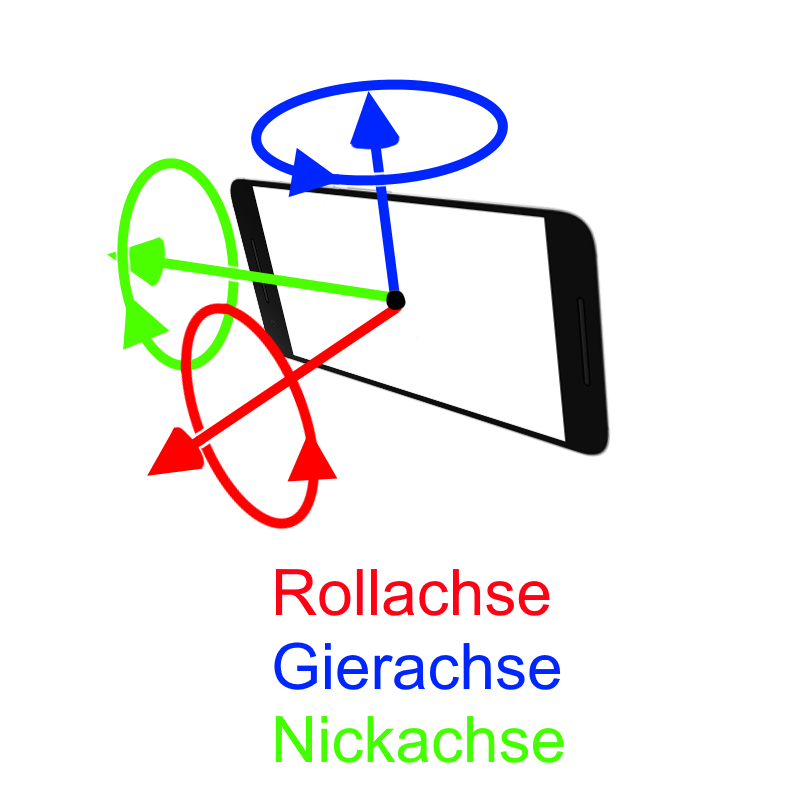
\includegraphics[width=0.5\linewidth]{Reviewdokument/Grafiken/drehachsen.png}
\end{figure}}}

\newglossaryentry{Detektion}{name={Detektion}, description={~\\Lokalisierung eines Merkmals (insb. eines Verkehrszeichens) in einem Bild}}

\newglossaryentry{Fahrzeug}{name={Fahrzeug}, description={~\\Handelsüblicher Personenkraftwagen (PKW), insbesondere kein Lastkraftwagen\\ (LKW)}}

\newglossaryentry{Filter}{name={Filter}, description={~\\Ein Verarbeitungsschritt. Jeder Filter hat eine Dateneingabe und eine -ausgabe. In jedem Verarbeitungsschritt werden die einkommenden Daten umgewandelt. Bei der Umwandlung können den Daten Teile entnommen, hinzugefügt oder auch vollständig ersetzt werden. Die Art der Umwandlung wird durch den Filter bestimmt}}

\newglossaryentry{Filterverwaltungs-Bibliothek}{name={Filterverwaltungs-Bibliothek}, description={~\\Programm-Bibliothek, welche Möglichkeiten bietet, Filter und Neuronale Filter zu laden und auf Bildserien anzuwenden}}

\newglossaryentry{FLOPs}{name={FLOPs}, 
description={Floating Point Operations.\\Operationen auf Fließkommazahlen, die von der \gls{ALU} ausgeführt werden. Sie gelten als eine der aufwendigsten, elementaren Operationen und bestimmen maßgeblich die Laufzeit eines Programms. Ausdrücklich zu unterscheiden von \glqq FLOPS\grqq}}

\newglossaryentry{FLOPS}{name={FLOPS}, 
description={Floating Point Operations per Second.\\Maß für die Leistungsfähigkeit von Computern. Ausdrücklich zu unterscheiden von \glqq FLOPs\grqq}}

\newglossaryentry{Geschwindigkeitsschild}{name={Geschwindigkeitsschild}, description={~\\Gibt die zulässige Höchstgeschwindigkeit des Fahrzeugs an, an dessen Rückseite es befestigt ist. Siehe §58 \gls{StVZO}}}

\newglossaryentry{GPU}{name={GPU}, 
description={Graphics Processing Unit; Grafikkarte.\\ Rechen- und Steuerwerk einer Rechenmaschine, hier insb. eines Personalcomputers oder eines Smartphones, welches auf die Bildverarbeitung spezialisiert ist}}

\newglossaryentry{Keras}{name={Keras}, description={~\\Deep-Learning-Framework in Python basierend auf TensorFlow}}

\newglossaryentry{Klassifikation}{name={Klassifikation}, description={~\\Einteilung eines Merkmals in eine Klasse von Urbildern}}

\newglossaryentry{Konfidenz}{name={Konfidenz}, description={~\\Sicherheit, dass das Objekt korrekt klassifiziert wurde}}

\newglossaryentry{Label}{name={Label}, description={~\\ Meta-Informationen zu einem Sample. In diesem Zusammhang die Position, Größe und Art von Verkehrsschildern in einer Bildaufnahme}}

\newglossaryentry{mAP}{name={mAP}, description={mean Average Precision.\\Maß für die Genauigkeit eines Objekt-Detektors und -Klassifikators. Basiert auf der Position und Größe des vermuteten Bildausschnitts sowie der Rangverteilung der vermuteten Klasse}}

\newglossaryentry{Multithreading}{name={Multithreading}, description={Nebenläufigkeit.\\ Gleichzeitiges Abarbeiten mehrerer Threads innerhalb eines Prozesses}}

\newglossaryentry{Neuronaler Filter}{name={Neuronale Filter}, description={~\\Ein Filter, dessen Umwandlungsvorgehen durch ein Neuronales Netz bestimmt wird}}

\newglossaryentry{Neuronales Netzwerk}{name={Neuronales Netzwerk}, description={~\\Hier im Besonderen: Künstliches Neuronales Netzwerk. Simplifiziertes Modell eines Nervensystems, bestehend aus künstlichen Neuronen, welche auf Computern trainiert werden, um komplexe Aufgaben im Bereich der künstlichen Intelligenz zu bewältigen}}

\newglossaryentry{Nutzer}{name={Nutzer}, description={~\\Der aktuelle Fahrzeugführer, während sich das Fahrzeug nicht in Fahrt befindet bzw. der Beifahrer, während sich das Fahrzeug in Fahrt befindet. Es wird das generische Maskulinum verwendet}}

\newglossaryentry{OpenCV2}{name={OpenCV2}, description={Open Source Computer Vision Library. \\Quelloffene Computergrafikbibliothek. Hier verwendet um Datensätze sowie das erfasste Kamerabild auf die Eingabespezifikationen der Neuronalen Netzwerke anzupassen}}

\newglossaryentry{Produkt}{name={Produkt}, description={~\\Die Kombination aus App und API, welche im Rahmen dieses Softwareprojektes entwickelt werden}}

\newglossaryentry{Pipe}{name={Pipe}, description={~\\Eine Pipe stellt eine Verbindung zwischen den einzelnen Verarbeitungsschritten dar}}

\newglossaryentry{Pipes and Filters}{name={Pipes and Filters}, description={auch Datenfluss-System.\\ Ein Architekturmuster welches die Struktur für Systeme, die Datenströme verarbeiten, darstellt}}

\newglossaryentry{Protobuf}{name={Protocol Buffers, Protobuf}, description={~\\Bezeichnet ein von Google entwickeltes, programmiersprachen- und plattformunabhängiges Format sowie die dazugehörige Implementierung für die Serialisierung und Deserialisierung strukturierter Daten.}}

\newglossaryentry{Sample}{name={Sample}, description={~\\In diesem Zusammenhang eine Bildaufnahme von Verkehrszeichen, welche Neuronalen Netzwerken präsentiert werden können, um sie zur Detektion und Klassifkation zu trainieren}}

\newglossaryentry{Smartphone}{name={Smartphone}, description={~\\Mobiles Endgerät, welches über eine integrierte Kamera verfügt und den im Pflichtenheft spezifizierten Bedingungen genügt}}

\newglossaryentry{SoC}{name={SoC}, description={System-on-a-Chip.\\ Kombination von CPU, Bus, Taktgeber, Co-CPUs, GPU, Soundchip, Interfaces, etc. oder Teilen davon auf einem Chip. Häufig verwendet in mobilen Endgeräten und eingebetteten Systemen um durch hohe Integrationsdichten Fläche auf der Platine einzusparen}}

\newglossaryentry{StVO}{name={StVO}, description={Straßenverkehrsordnung\footlink{https://www.gesetze-im-internet.de/stvo\_2013/StVO.pdf}{29.04.2018}}}

\newglossaryentry{StVZO}{name={StVZO}, description={Straßenverkehrszulassungsordnung\footlink{https://www.gesetze-im-internet.de/stvzo\_2012/StVZO.pdf}{29.04.2018}}}

\newglossaryentry{System}{name={System}, description={~\\Gesamtheit aus Halterung, Smartphone und App}}

\newglossaryentry{Tracking}{name={Tracking}, description={~\\Objekte anhand primitiver Merkmale in einer Bildserie oder einem Video lokalisieren und verfolgen}}

\newglossaryentry{TensorFlow Lite}{name={TensorFlow Lite}, description={~\\Für mobile Endgeräte optimiertes Deep-Learning-Framework des Google Brain Teams\footlink{https://www.tensorflow.org/mobile/tflite/}{29.04.2018}}}

\newglossaryentry{TensorFlow Mobile}{name={TensorFlow Mobile}, description={~\\Deep-Learning-Framework des Google Brain Teams, welches zwar für Android noch keine GPU Unterstützung bietet, dafür aber derzeit noch bzgl. der Kompatibilität besser von bereits etablierten Netzwerken unterstützt wird}}

\newglossaryentry{Tensorflow Node}{name={Tensorflow Node},description={~\\Ein Knoten (Node) im Sinne von TensorFlow bezeichnet eine bestimmte Operation innerhalb des Netzwerk Models: Es ist die grundlegende Einheit für Berechnungen innerhalb von TensorFlow. Die Ergebnisse dieser Knoten lassen sich anhand deren Bezeichnungen (zum Beispiel \glqq{}final\_output\qrqq{})  einzeln abfragen}}

\newglossaryentry{UI}{name={UI},description={User Interface.\\ Benutzeroberfläche}}

\newglossaryentry{VZ}{name={VZ}, description={Verkehrszeichen}}

\newglossaryentry{Verkehrszeichen-API}{name={Verkehrszeichen-API}, description={~\\Besondere Programmierschnittstelle, die für Verkehrszeichenerkennung optimiert ist und erweiterte Logik zur Verfügung stellt, wie etwa die Abschätzung, wann ein Verkehrsschild passiert wurde und damit gültig ist und angezeigt werden muss}}

\newglossaryentry{Verkehrszeichenkombination}{name={Verkehrszeichenkombination}, description={~\\Gruppe von untereinander angebrachten Verkehrszeichen, welche einen gemeinsamen Sinnzusammenhang darstellen}}

\newglossaryentry{VwV-StVO}{name={VwV-StVO}, description={Allgemeine Verwaltungsvorschrift
zur Straßenverkehrs-Ordnung\footlink{http://www.verwaltungsvorschriften-im-internet.de/bsvwvbund\_26012001\_S3236420014.htm}{29.04.2018}}}



\author{
    [Projektgruppe 2]\\~\\
    \textit{Namen entfernt}\\~\\
    \textcolor{red}{Verwendung nur zu Lehrzwecken an der TU Ilmenau. Die Verwendung}\\\textcolor{red}{für private oder kommerzielle Zwecke ohne Einwilligung der Autoren ist}\\ \textcolor{red}{ausdrücklich untersagt.}\\~\\
    Kontakt: \href{mailto:signapse.app@gmail.com}{signapse.app@gmail.com}
    %Bock, Robert Niklas\\ \texttt{robert-niklas.bock@tu-ilmenau.de}\\~\\
    %Dirbas, Mohammad\\ \texttt{mohammad.dirbas@tu-ilmenau.de} \\~\\
    %Fischedick, Söhnke Benedikt\\ \texttt{soehnke-benedikt.fischedick@tu-ilmenau.de} \\~\\
    %Hampel, Jakob Frank\\ \texttt{jakob.hampel@tu-ilmenau.de} \\~\\
    %Köhler, Florian\\ \texttt{florian.koehler@tu-ilmenau.de} \\~\\
    %Langer, Patrick\\ \texttt{patrick.langer@tu-ilmenau.de} \\~\\
    %Nowati, Yusuf\\ \texttt{yusuf.nowati@tu-ilmenau.de} \\~\\
    %Treichel, Tim\\ \texttt{tim.treichel@tu-ilmenau.de} \\ ~\\ ~\\ ~\\ ~\\
}


\title{Reviewdokument\\Verkehrszeichenerkennung}

\begin{document}
\maketitle

\renewcommand{\arraystretch}{1.5}

%\clearpage

\addtocounter{page}{-1}
\topskip0pt
\vspace*{\fill}

\begin{center}
%Dieses Dokument ist für die Verwendung mit %\href{https://get.adobe.com/de/reader/}{Adobe$^{\tiny{\text{\textregistered}}}$ %Reader$^{\tiny{\text{\textregistered}}}$} optimiert.\\
%\href{https://get.adobe.com/de/reader/}{https://get.adobe.com/de/reader/} \\
{\bfseries Temporärer Disclaimer!}\\
~\\
Dieses Dokument wurde zuletzt von Söhnke und Robert am 01.05.2018 um 23:44 Uhr auf Rechtschreib-, Grammatik-, Struktur-, Logik- und Crossreferencing-Fehler untersucht. Wer nach diesem Datum Änderungen durchführt ist für die Integrität selbst verantwortlich und wird von uns höchstpersönlich \underline{gelyncht}, wenn er es versäumt diese zu bewahren!\\
~\\
{\bfseries Vor Abgabe Entfernen!}\\
\end{center}
\vspace*{\fill}

\tableofcontents

\chapter*{Einleitung}
\addcontentsline{toc}{chapter}{Einleitung}
Ziel dieses Softwareprojektes ist es, ein \gls{System} (bestehend aus einem \gls{Smartphone}, einer KFZ-Smartphonehalterung und einer \gls{App}) zur Verkehrszeichenerkennung zu entwickeln, welches in jedem \gls{Fahrzeug} nachgerüstet werden kann. Die Erkennung soll dabei in der Lage sein, die Geschwindgkeitsregulierung von Verkehrszeichen festzustellen.\\

Inhalt der dafür zu entwickelnden \gls{App} ist eine Benutzer-Schnittstelle, welche erkannte Verkehrszeichen während der Fahrt anzeigt, sowie eine Logik-Schnittstelle, welche in Echtzeit aus Kameraaufnahmen Verkehrszeichen identifiziert. Die Logik-Schnittstelle soll dabei derart modular aufgebaut sein, sodass auch andere Detektionsprobleme damit lösbar sind.\\

Um den Einsatz dieser Schnittstelle auch auf anderen Plattformen zu ermöglichen, ist sie dabei unabhängig von der Android API in C++ umzusetzen.\\

Die App soll dafür genutzt werden, die rückseitig eingebaute Kamera des Smartphones anzusprechen und der Logik-Schnittstelle die entsprechende Aufnahme zu übergeben.
Die darauf folgende Verarbeitung der Aufnahme, bis hin zur korrekten Anzeige des erkannten Verkehrszeichens, wird in drei Teilprobleme aufgeteilt.
Der erste Schritt stellt dabei die Detektion von Verkehrszeichen dar. Bei dieser wird festgestellt, wo sich in der Aufnahme potenziell Verkehrszeichen befinden.\\
Im Anschluss werden die detektierten Ausschnitte in einem weiteren Schritt, der Klassifikation, entsprechenden Klassen zugeordnet und damit identifiziert.\\
Als dritter und letzter Schritt wird in der App das Ergebnis der Klassifikation angezeigt, sodass für den Endbenutzer leicht die derzeit gültige Höchstgeschwindigkeit ersichtlich ist.\\
Die App wird dabei den Endbenutzer bei einer Überschreitung der zulässigen maximalen Geschwindigkeit warnen.\\

Da sowohl die Detektion als auch die Klassifikation komplexe Probleme darstellen, welche mit klassischen algorithmischen Ansätzen nur äußerst schwierig zu bearbeiten sind, wird hier eine Lösung mittels Neuronaler Netzwerke angesetzt.

%Die Umsetzung der \gls{Detektion} und \gls{Klassifikation} soll mittels \glslink{Neuronales Netzwerk}{Neuronaler Netzwerke} erfolgen, dabei ist die \glslink{Deep Learning}{Deep-Learning-Strategie} zu verfolgen.

%%%%%%%%%%%%%%%%%%%%%%%%%%%%%%%%%%%%%%%%%%%%%%%%%%%
%%%%%%%%%%%%%%%%%% P H A S E - 2 %%%%%%%%%%%%%%%%%%
%%%%%%%%%%%%%%%%%%%%%%%%%%%%%%%%%%%%%%%%%%%%%%%%%%%
%\def\partname{Phase}
\part[Projektplanung Phase II]{Projektplanung}
%\def\partname{Teil}

\chapter{Änderungen an den Planungen aus Phase I}
%Unter \cref{subsec:projektplan} wurde grob der Aufwand für das \glslink{Label}{Labeln} der aufgenommenen \glslink{Sample}{Rohdaten} sowie für das Implementieren abgeschätzt. Es stellte sich heraus, dass die 50 Personenstunden (d.h. knapp über 6 h pro Person) für das \glslink{Label}{Labeln} eine grobe Fehleinschätzung waren. Für das Aussortieren wurden \textit{pro Person} im Mittel 2 h gebraucht und für das \glslink{Label}{Labeln} an sich zusätzlich noch einmal 23 h pro Person. Dazu kam, dass die zur Weiterverarbeitung notwendigen Python-Skripte in der ursprünglichen Abschätzung komplett ignoriert wurden. Im Endeffekt belief sich der Aufwand für den Meilenstein Samples auf 300 Personenstunden. Dementsprechend sind die nachfolgenden Meilensteine jeweils eine Woche nach hinten gerückt. Einen Teil dieser Verzögerungen lässt sich auf fehlerhafte Zeitabschätzungen zurückführen, ein weiterer Teil darauf, dass deutlich mehr \glslink{Sample}{Samples} \glslink{Label}{gelabelt} wurden, als ursprünglich veranschlagt, was aber erst nach dem \glslink{Label}{Labeln} aufgefallen ist. Dies lag unter Anderem daran, dass die Verkehrszeichendichte in dem aufgenommenen Videomaterial größer als gedacht war, und sich so mehr \gls{Sample}s  als ursprünglich geplant extrahieren ließen. Allerdings wurden die Samples erst nach dem vollständigen Labeln zusammengezählt, sodass dies erst am Ende auffiel.\\

\section{Rückblickende Beurteilung der Aufwandsabschätzung für den Datensatz}
\label{sec:aufwandsabschaetzung2}
Wie sich im Nachhinein zeigte, waren die Schätzungen für den Aufwand zur Erstellung des Datensatzes deutlich zu optimistisch gewählt. Vor allem die Labelrate ($l$) wich schwerwiegend von den Berechnungen ab. Sie war auf Basis der Leistung einer überdurchschnittlich schnellen Person aus der Gruppe geschätzt worden. Dies stellte nicht die mittlere Labelrate innerhalb der Gruppe dar. Ferner ließ die Einschätzung wichtige Effekte außer Acht: beispielsweise wurde es für vorteilhaft erachtet, alle Verkehrszeichen zu labeln, auch wenn diese auf die Geschwindigkeitsbeschränkung keinen Einfluss haben. Der Grund dafür ist, dass einige sehr unüblich gefärbte Verkehrszeichen, beispielsweise der Vorwegweiser, gegebenenfalls später als ähnliche Verkehrszeichen - z.B. die Orstafel - klassifiziert werden könnten, weil dem \glslink{Neuronales Netzwerk}{Neuronalen Netzwerk} nur die Ortstafel präsentiert wurde und keine Abgrenzung zu den ähnlichen Zeichen stattgefunden hat.\\
Des Weiteren ist das Erstellen und Optimieren der Python-Skripte - welche den Datensatz aus den Einzelbildern extrahieren, in andere Formate umrechnen, Skalierungen durchführen, Label-Klassen von natürlicher Sprache in fortlaufende Nummerierungen übersetzen sowie alle verwendeten Datensätze in einen Gesamtdatensatz zusammenführen - bei der Aufwandsabschätzung überhaupt nicht mit in Betracht gezogen worden.\\
All diese Faktoren haben zu einem massiv erhöhten Zeitaufwand für das Labeln der Samples geführt.\\

%______ COPY CAT
%wurde es für vorteilhaft erachtet, alle Verkehrszeichen zu labeln, auch wenn diese auf die Geschwindigkeitsbeschränkung keinen Einfluss haben. Der Grund dafür ist, dass einige sehr unüblich gefärbte Verkehrszeichen, bspw. der Vorwegweiser, ggf. später als ähnliche Verkehrszeichen - z.B. die Orstafel - klassifizieren werden könnten, weil dem \glslink{Neuronales Netzwerk}{Neuronalen Netzwerk} nur die Ortstafel präsentiert wurde und keine Abgrenzung zu den ähnlichen Schildern stattgefunden hat.\\
%In \cref{sec:eigens_gelabelte_verkehrszeichen} ist eine Liste der dem ursprünglichen Datensatz (sh. \cref{sec:datensatz}) hinzugefügten Verkehrszeichen zu finden.\\
%______ COPY CAT

\subsubsection*{Aufnahme des Videomaterials}
Auf den durchgeführten Testfahrten wurde etwa \SI{6.5}{\hour} Videomaterial erzeugt. Bei der konstanten Framerate von \SI{3}{\hertz} beläuft sich damit die Zahl an Rohbildaufnahmen auf etwa \SI{70000}{}. Damit konnten deutlich mehr Bilder aufgenommen werden, als in der ursprünglichen Schätzung gefordert. Allerdings wurden von diesen insgesamt \SI{55000}{} Aufnahmen verworfen, da sie keine Verkehrszeichen beinhalteten. Damit beläuft sich der (experimentell bestimmte) Faktor $Q$ auf $\frac{\SI{70000}{} - \SI{55000}{}}{\SI{70000}{}} = \SI{0.214}{}$ und liegt damit deutlich höher als die Schätzung. Dabei ist zu beachten, dass dieser alle Verkehrszeichen berücksichtigt, demnach auch solche ohne Einfluss auf die derzeitig erlaubte Höchstgeschwindigkeit wie beispielsweise Vorwegweiser oder Vorfahrtsschilder. Zudem beschreibt er den Anteil individueller Frames in einer Aufnahme, nicht die Häufigkeit der physischen Schilder auf einer gegebenen Strecke. Es war ursprünglich gewünscht, möglichst viele individuelle Schilder aufzunehmen, anstatt dieselben aus unterschiedlichen Blickwinkeln. Aufgrund der zeitlichen und wirtschaftlichen Einschränkungen (kein Budget zum Decken der Benzinkosten) ließ sich dies allerdings nur bedingt realisieren.\\

\subsubsection*{Weiterverarbeitung der Daten}
Das Aussortieren der Verkehrszeichen wurde bemerkenswert gut abgeschätzt und hat genau die berechneten \SI{16}{\PS} benötigt.\\
Die Dauer des Labelns der Verkehrszeichen wurde deutlich unterschätzt. Der Aufwand belief sich auf insgesamt rund \SI{184}{\PS}, also \SI{23}{\hour} pro Person - das Neunfache (!) der ursprünglichen Schätzung. Darauf basierend ergibt sich eine mittlere Labelrate $l$ von \SI{81.52}{\per\hour}.\\

Der Aufwand zum Erstellen der Python-Skripte wird im Nachhinein mit etwa \SI{100}{\PS} bemessen.\\

\subsubsection*{Konsequenzen}
Schlussendlich belief sich der Aufwand bezüglich des Meilensteins \glqq{}Samples\grqq{} auf 300 PS. Dementsprechend wurden die nachfolgenden Meilensteine jeweils um eine Woche aufgeschoben. Es musste deshalb an anderen Meilensteinen Bearbeitungszeit eingespart werden, da die Richtlinien des Agilen Vorgehens keine Überstunden vorsehen.\\
Nach einer Risiko-Aufwandsabschätzung wurde entschieden, das im Grobentwurf (sh. \cref{subsec:kontrollfluss}) beschriebene \gls{Tracking} aus Zeitgründen vorerst hinten anzustellen. Ob das \gls{Tracking} überhaupt implementiert wird, soll in der nächsten Phase unter Berücksichtigung der zur Verfügung stehenden Zeit entschieden werden.\\

\section{Abgeänderter Projektplan}

Die grüne, gestrichelte Linie in Abb. 1.1 zeigt den aktuellen Stand des Projektes an.\\
\begin{figure}[H]
\centering
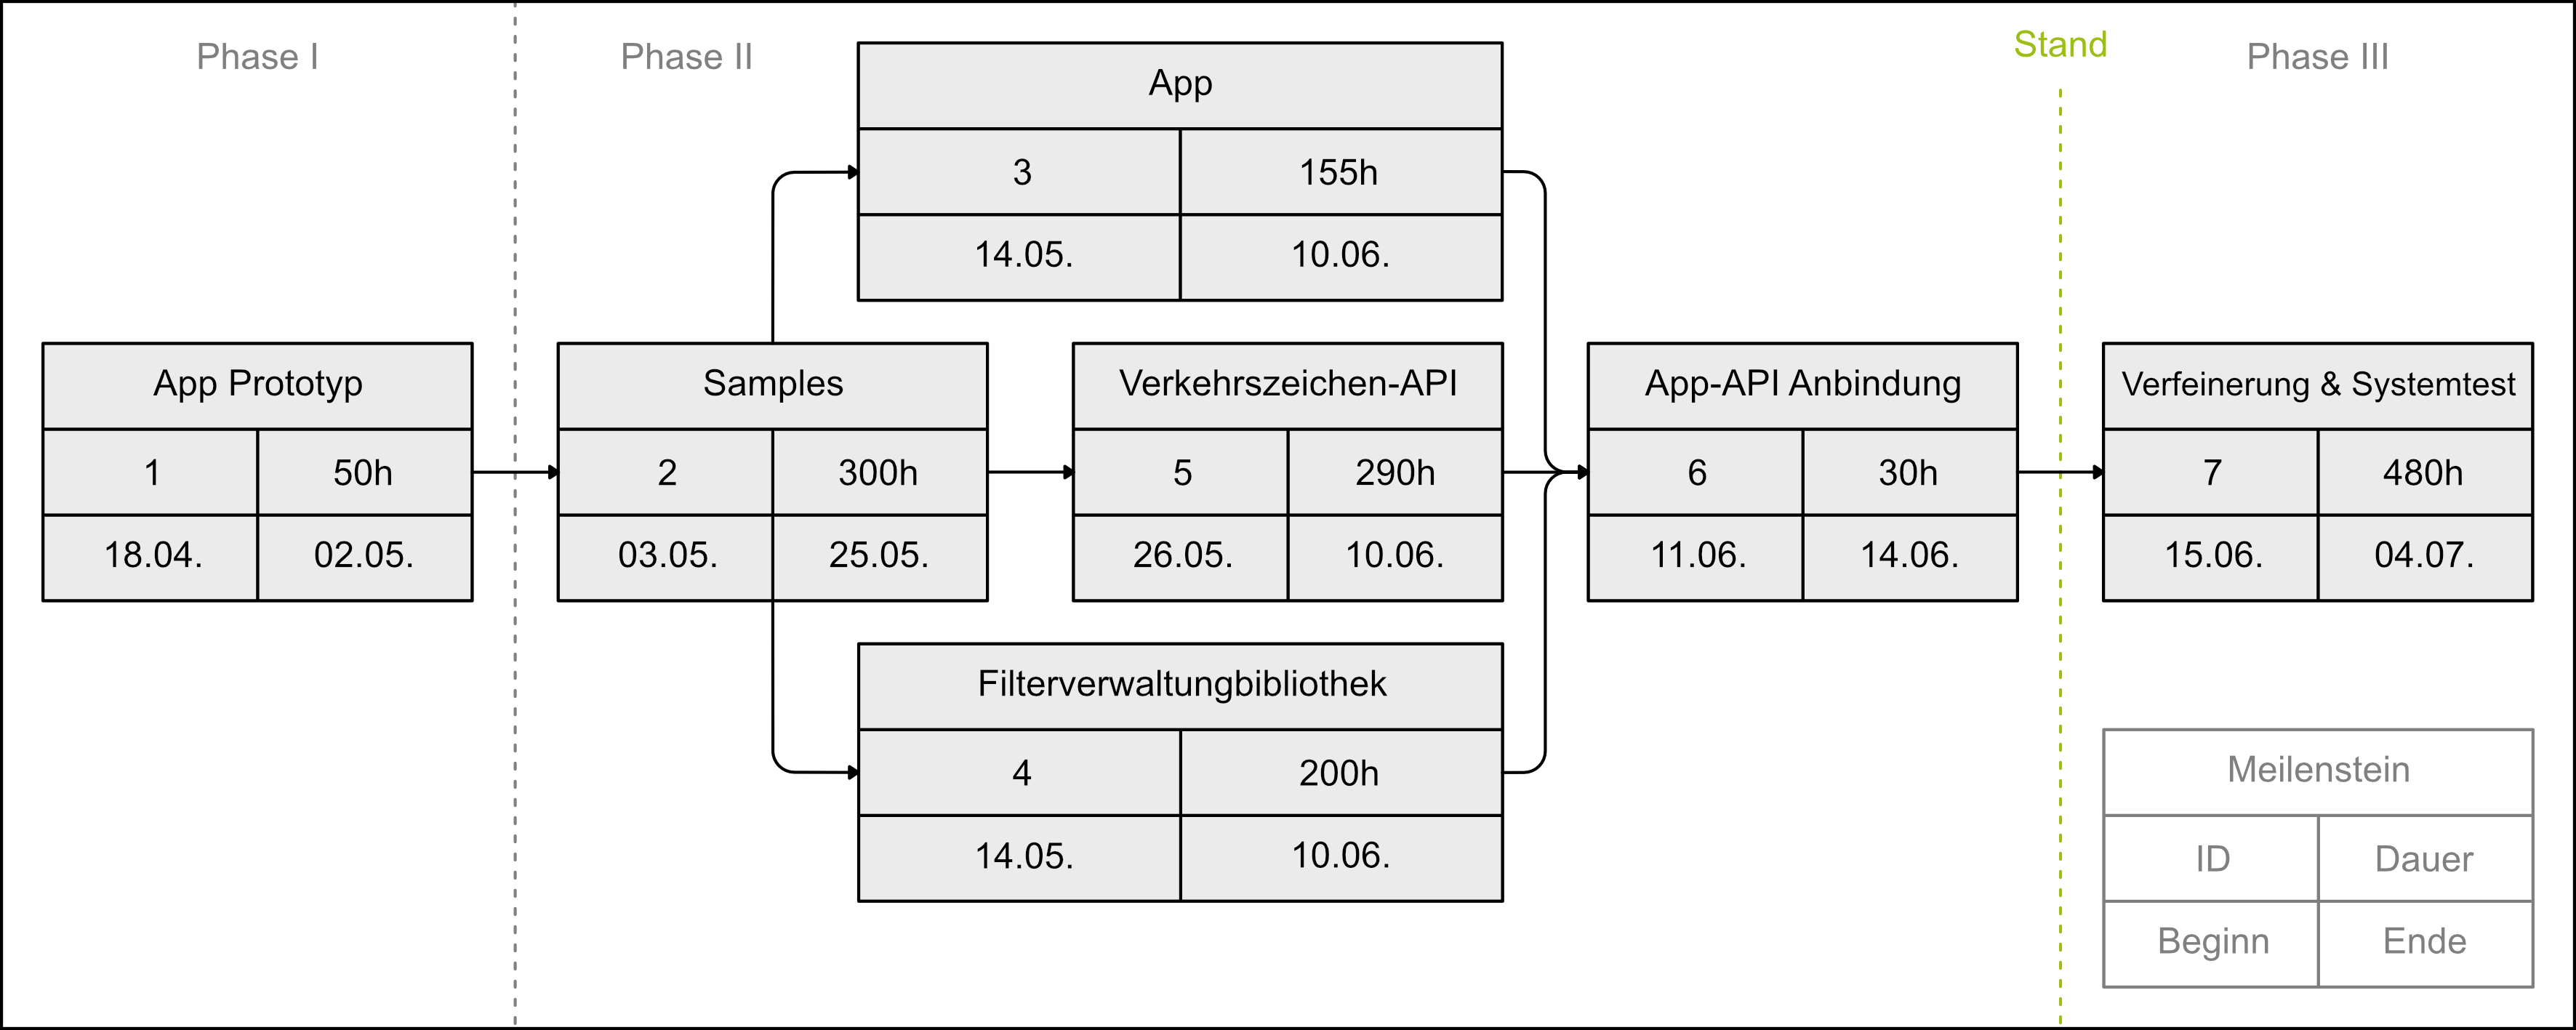
\includegraphics[width=1\linewidth]{Reviewdokument/Grafiken/project_plan_v2.png}
\caption{Projektplan mit aktualisierten Abschätzungen für die Meilensteine}
\end{figure}

\chapter{Ergebnisse der zweiten Iteration}

\section[Meilenstein 1: App Prototyp]{Meilenstein 1: App Prototyp, bis 02.05 (50 PS)}
Der Prototyp wurde zum Ende von Phase I erstellt und wurde seitdem ständig weiterentwickelt.\\

\section[Meilenstein 2: Aufnahme und Labeln aller Samples]{Meilenstein 2: Aufnahme und Labeln aller Samples, bis 10.06. (300 PS)}

Die \glslink{Sample}Samples wurden aufgenommen, komplett gelabelt und sortiert. Wie im \cref{sec:aufwandsabschaetzung2} beschrieben, hat dies deutlich länger gedauert als ursprünglich geplant. Neben den in \cref{sec:liste_zu_erkennende_verkehrszeichen} spezifizierten Verkehrszeichen wurden auch einige spezielle Gefahrenzeichen gelabelt. Dies liegt darin begründet, dass diese Gefahrenzeichen einen Einfluss auf die zulässige Höchstgeschwindigkeit haben, wenn sie an dem selben Mast hängen und damit den Geltungsbereich  eines geschwindigkeitsregulierenden Verkehrszeichens einschränken. Dies ist jedoch erst im Verlauf des Labelns aufgefallen.\\

Ferner wurde es für vorteilhaft erachtet, alle Verkehrszeichen zu labeln, auch wenn diese auf die Geschwindigkeitsbeschränkung keinen Einfluss haben. Der Grund dafür ist, dass einige sehr unüblich gefärbte Verkehrszeichen, bspw. der Vorwegweiser, ggf. später als ähnliche Verkehrszeichen - z.B. die Orstafel  - klassifizieren werden könnten, weil dem \glslink{Neuronales Netzwerk}{Neuronalen Netzwerk} nur die Ortstafel präsentiert wurde und keine Abgrenzung zu den ähnlichen Schildern stattgefunden hat.\\
In \cref{sec:eigens_gelabelte_verkehrszeichen} ist eine Liste der dem ursprünglichen Datensatz (sh. \cref{sec:datensatz}) hinzugefügten Verkehrszeichen zu finden.\\
 
\section[Meilenstein 3: App]{Meilenstein 3: App, bis 10.06. (155 PS)}
Dieser Meilenstein beinhaltet die \gls{App}, allerdings noch ohne Einbindung der \gls{API}. Der Meilenstein 3 ist erreicht, wenn das \gls{UI} vorhanden ist, die Kameraanbindung sowie die Geschwindigkeitsmessung funktioniert und wenn eine Möglichkeit zur Kalibrierung des Gerätes mittels Gravitationssensor oder Gyroskop vorhanden ist. Das \gls{UI} wurde bereits in der letzten Iteration begonnen.\\

\begin{figure}[H]
\centering
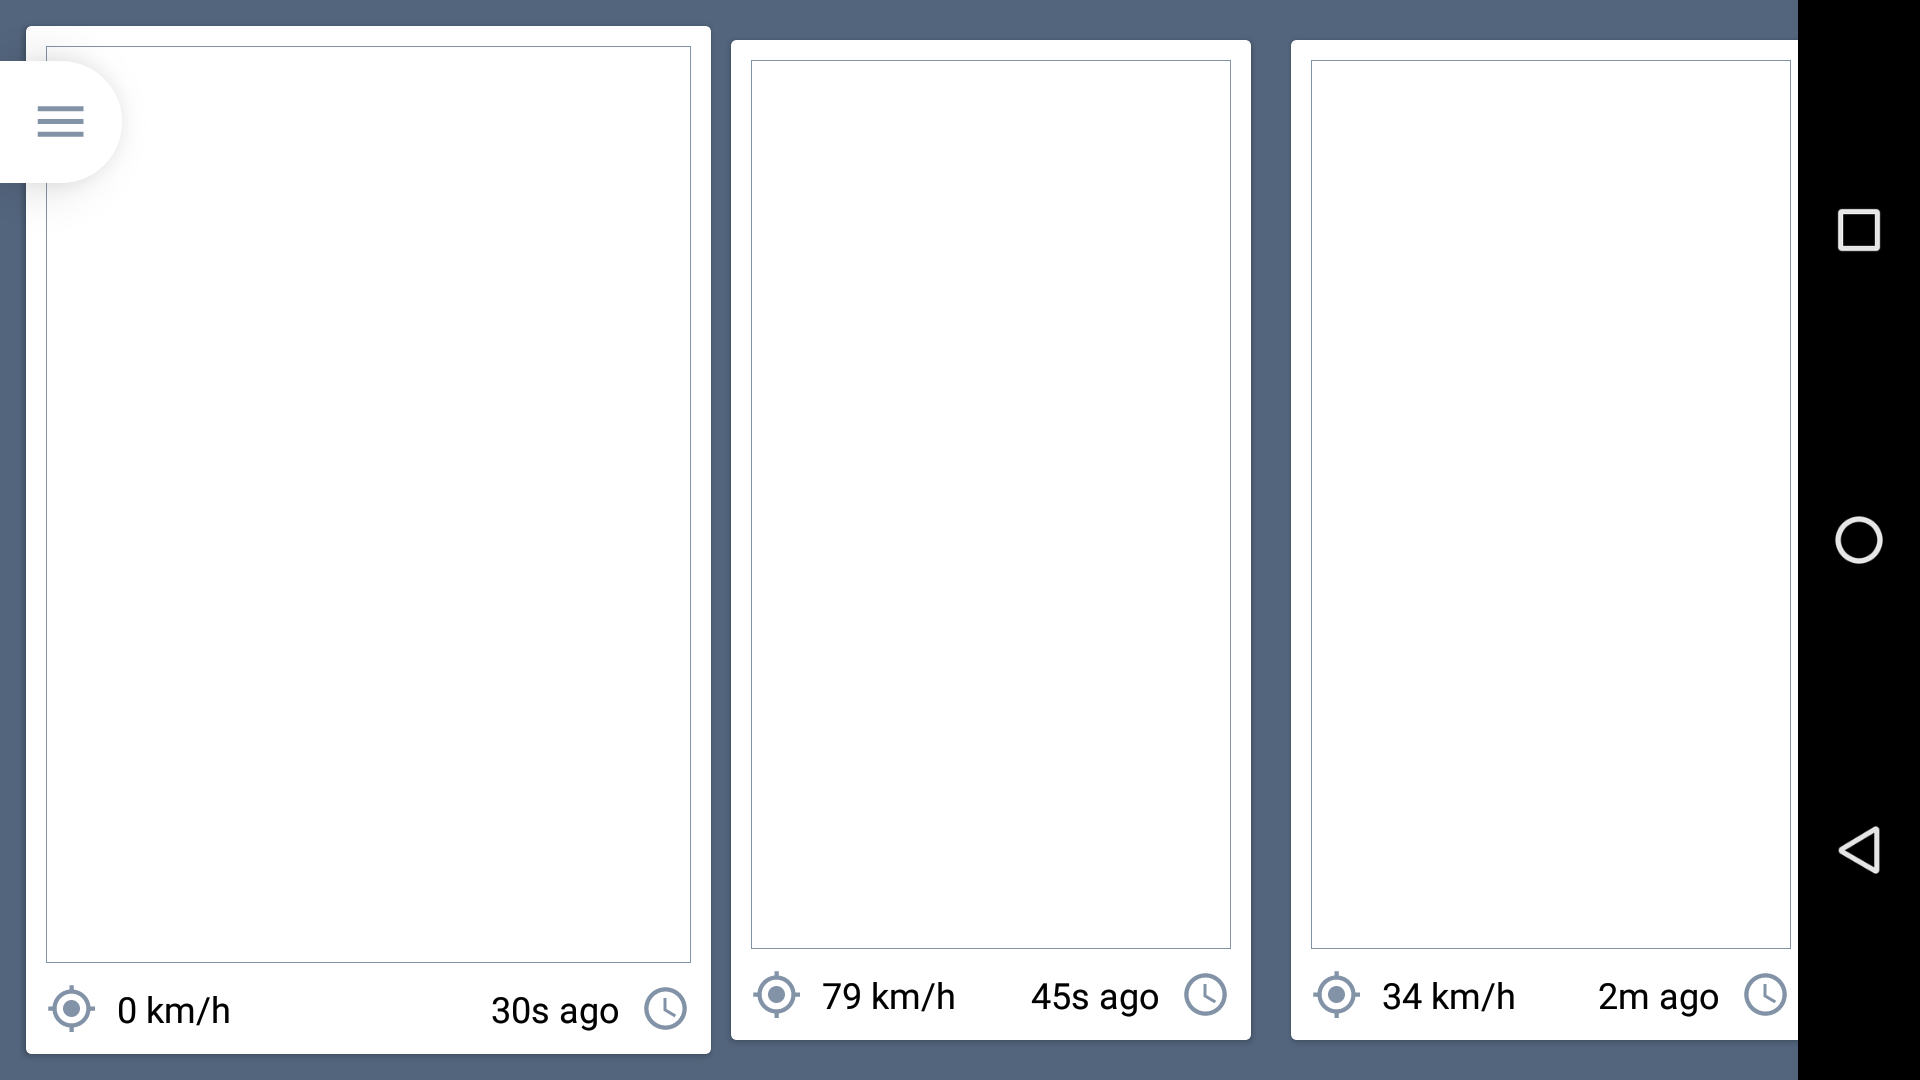
\includegraphics[width=0.9\linewidth]{Reviewdokument/Grafiken/app_detector_screenshot_old.png}
\caption{\gls{UI} des Detektor-Fragmentes zu Ende der ersten Iteration}
\label{fig:detektor_ui}
\end{figure}

Die Kameraanbindung stellte ein großes Problem dar, wurde aber termingerecht fertiggestellt und funktioniert wie gefordert(Pflichtenheft P4302). Während der Implementierung wurde temporär ein weiteres, nicht im Feinentwurf (sh. \cref{part:feinentwurf}) aufgelistetes Fragment eingefügt - \texttt{TSDDebugFragment} - welches Informationen über die \gls{Smartphone}-Kamera bereitstellt. Beispielsweise werden dort die verschiedenen Kameras, die verschiedenen Autofokus-Modi der jeweiligen Kameras sowie das aktuelle Kamerabild angezeigt. Wie der Name bereits vermuten lässt, dient dieses Fragment ausschließlich zum Debugging und wird \textit{voraussichtlich nicht} Teil der fertigen \gls{App} werden.\\

\begin{figure}[H]
\centering
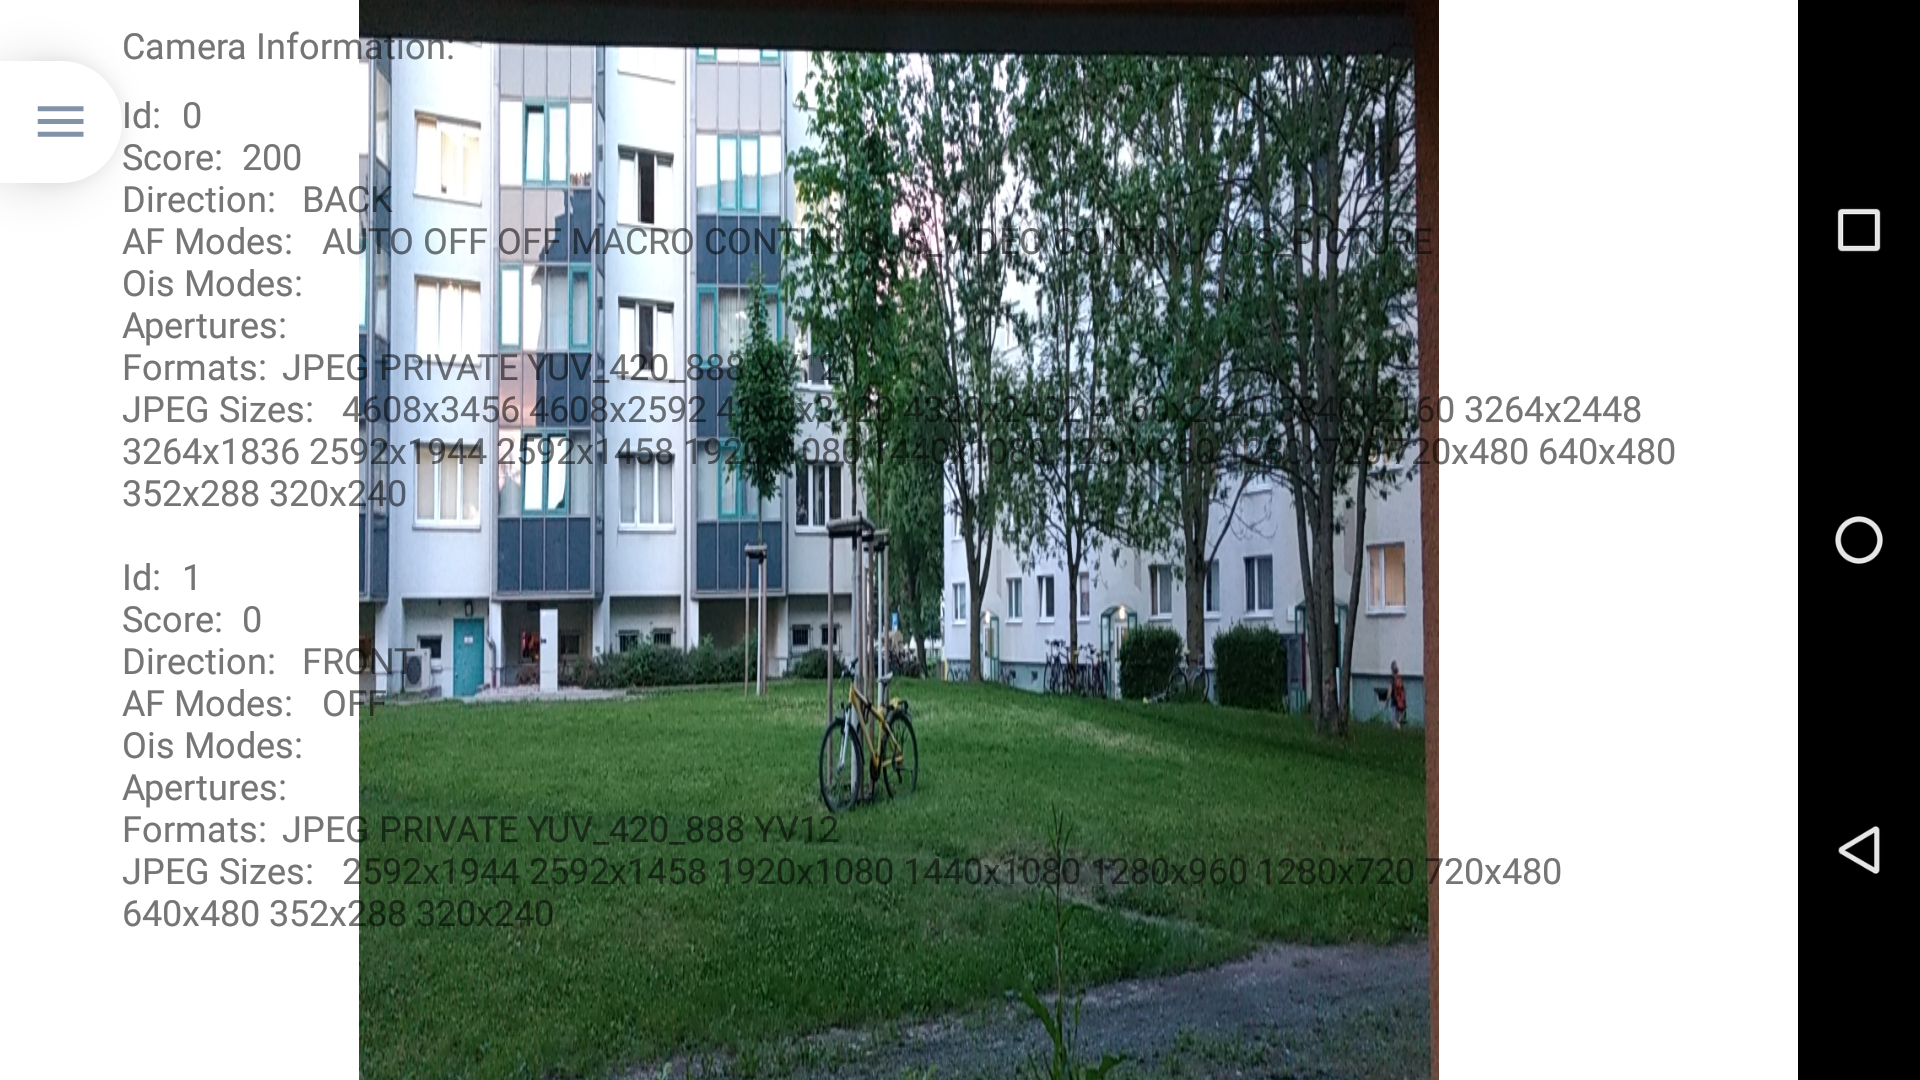
\includegraphics[width=0.9\linewidth]{Reviewdokument/Grafiken/app_debug_screenshot.png}
\caption{Debug-Fragment der App}
\end{figure}

Die GPS-Geschwindigkeitsermittelung wurde ebenfalls fertiggestellt. Dabei wurde von der Methode \texttt{onLocationChanged()} des Android-Frameworks gebraucht gemacht, welche automatisch aufgerufen wird, sobald das GPS eine Ortsänderung feststellt. Um die Geschwindigkeit zu errechnen, wird aus den GPS-Daten (Längen- und Breitengrad) die zurückgelegte Distanz in Meter bestimmt und durch die seit dem letzten Methodenaufruf vergangene Zeit dividiert. Erste Tests der GPS-Geschwindigkeitsermittelung im Vergleich mit einer Navigationsapp mit Geschwindigkeitsanzeige\footnote{\link{https://www.tomtom.com/de\_de/drive/sat-nav-app/go-mobile/}, 12.06.2018} zeigten, dass diese mit hinreichender Genauigkeit funktioniert. Um Ausreißer durch fehlerhafte Standortsermittelung zu vermeiden, werden die gemessenen Geschwindigkeiten in einen Ringspeicher geladen und die angezeigte Geschwindigkeit wird aus diesem gemittelt(Pflichtenheft P4304, B6007, B6009).\\

Da \glslink{Neuronales Netzwerk}{Neuronale Netze} oft sehr empfindlich auf Drehung des Eingaberaumes reagieren, ist es nötig, dass das \gls{Smartphone} während der Fahrt möglichst waagerecht hängt. Dazu wurde in der \gls{App} ein Kalibrierungsmenü umgesetzt, was dem \gls{Nutzer} vermitteln soll, ob das \gls{System} korrekt kalibriert ist oder nicht(Pflichtenheft P4306). Zunächst war geplant, dies mit dem Drehvektorsensor\footnote{\link{https://developer.android.com/guide/topics/sensors/sensors\_motion#sensors-motion-rotate}, 08.06.2018} umzusetzen, was sich aber als unnötig kompliziert erwies. Um aus dem Drehvektor die Neigung um die Y-Achse zu ermitteln, sind eine Reihe von Matrixoperationen notwendig, außerdem ist der Drehvektorsensor unter Umständen (z.B. wenn sich in der Nähe eine Magnetfeldquelle befindet) nicht besonders genau. Würde man sich für die Ausrichtung des \gls{Smartphone}s im Raum interessieren, wäre das die richtige Lösung gewesen. Für die Kalibrierung ist aber nur die Neigung um die Y- und Z-Komponente notwendig. Deshalb wurde sich für den G-Sensor\footnote{\link{https://developer.android.com/guide/topics/sensors/sensors\_motion#sensors-motion-grav}, 08.06.2018} entschieden, wobei mittels einer Arkustangens-Berechnung die gesuchten Drehwinkel bestimmt werden. Das \gls{System} ist korrekt kalibriert, falls das \gls{Smartphone} jeweils nicht mehr als 5° um die \glslink{Drehachsen}{Nick- und Rollachse} gedreht ist.\\

Bei dem \gls{UI} wurde sich zunächst an das Mockup gehalten, wie aus \cref{fig:detektor_ui} ersichtlich ist. Damit das Layout aber übersichtlicher wird - insbesondere sollen keine UI-Elemente von dem aktuell erkannten Verkehrszeichen ablenken - wurde es jedoch noch einmal komplett überarbeitet. Der Fokus bei dem Redesign lag darauf, das \gls{UI} etwas lebhafter zu gestalten, aber gleichzeitig nicht so farbenfroh, dass es von den wichtigen Informationen ablenkt. Das zuletzt erkannte Verkehrszeichen soll weiterhin das \gls{UI} dominieren(Pflichtenheft B6001, B6002, B6003, B6004).\\

Des Weiteren wurde ein Warnhinweis beim Start der \gls{App} implementiert, welcher dem Nutzer vermittelt, dass die \gls{App} kein Ersatz für Aufmerksamkeit am Steuer ist und dass deren Anwendung nur innerhalb der geltenden StVO erfolgen darf(Pflichtenheft P4307).

\begin{figure}[H]
\centering
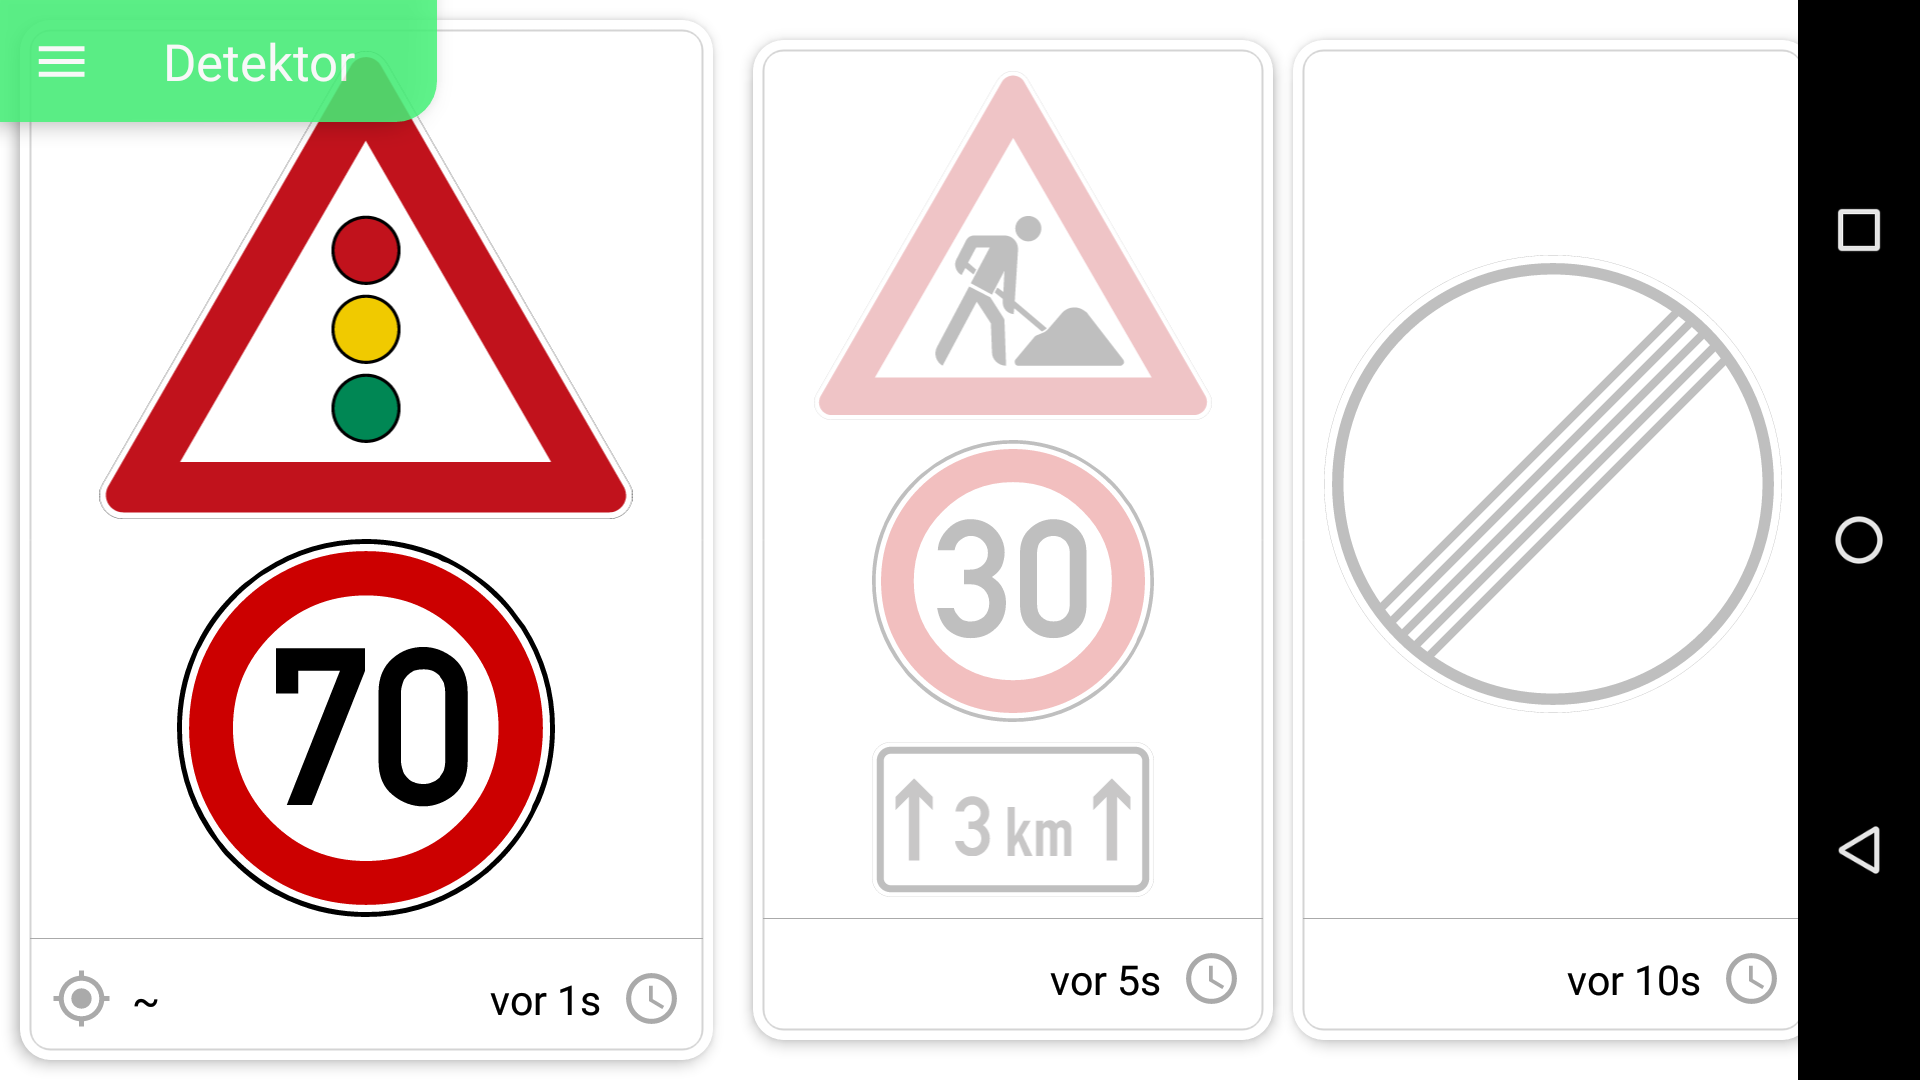
\includegraphics[width=0.9\linewidth]{Reviewdokument/Grafiken/app_detektor_neu.png}
\caption{UI des Detektor-Fragmentes zu Ende der zweiten Iteration}
\end{figure}


\begin{figure}[H]
\centering
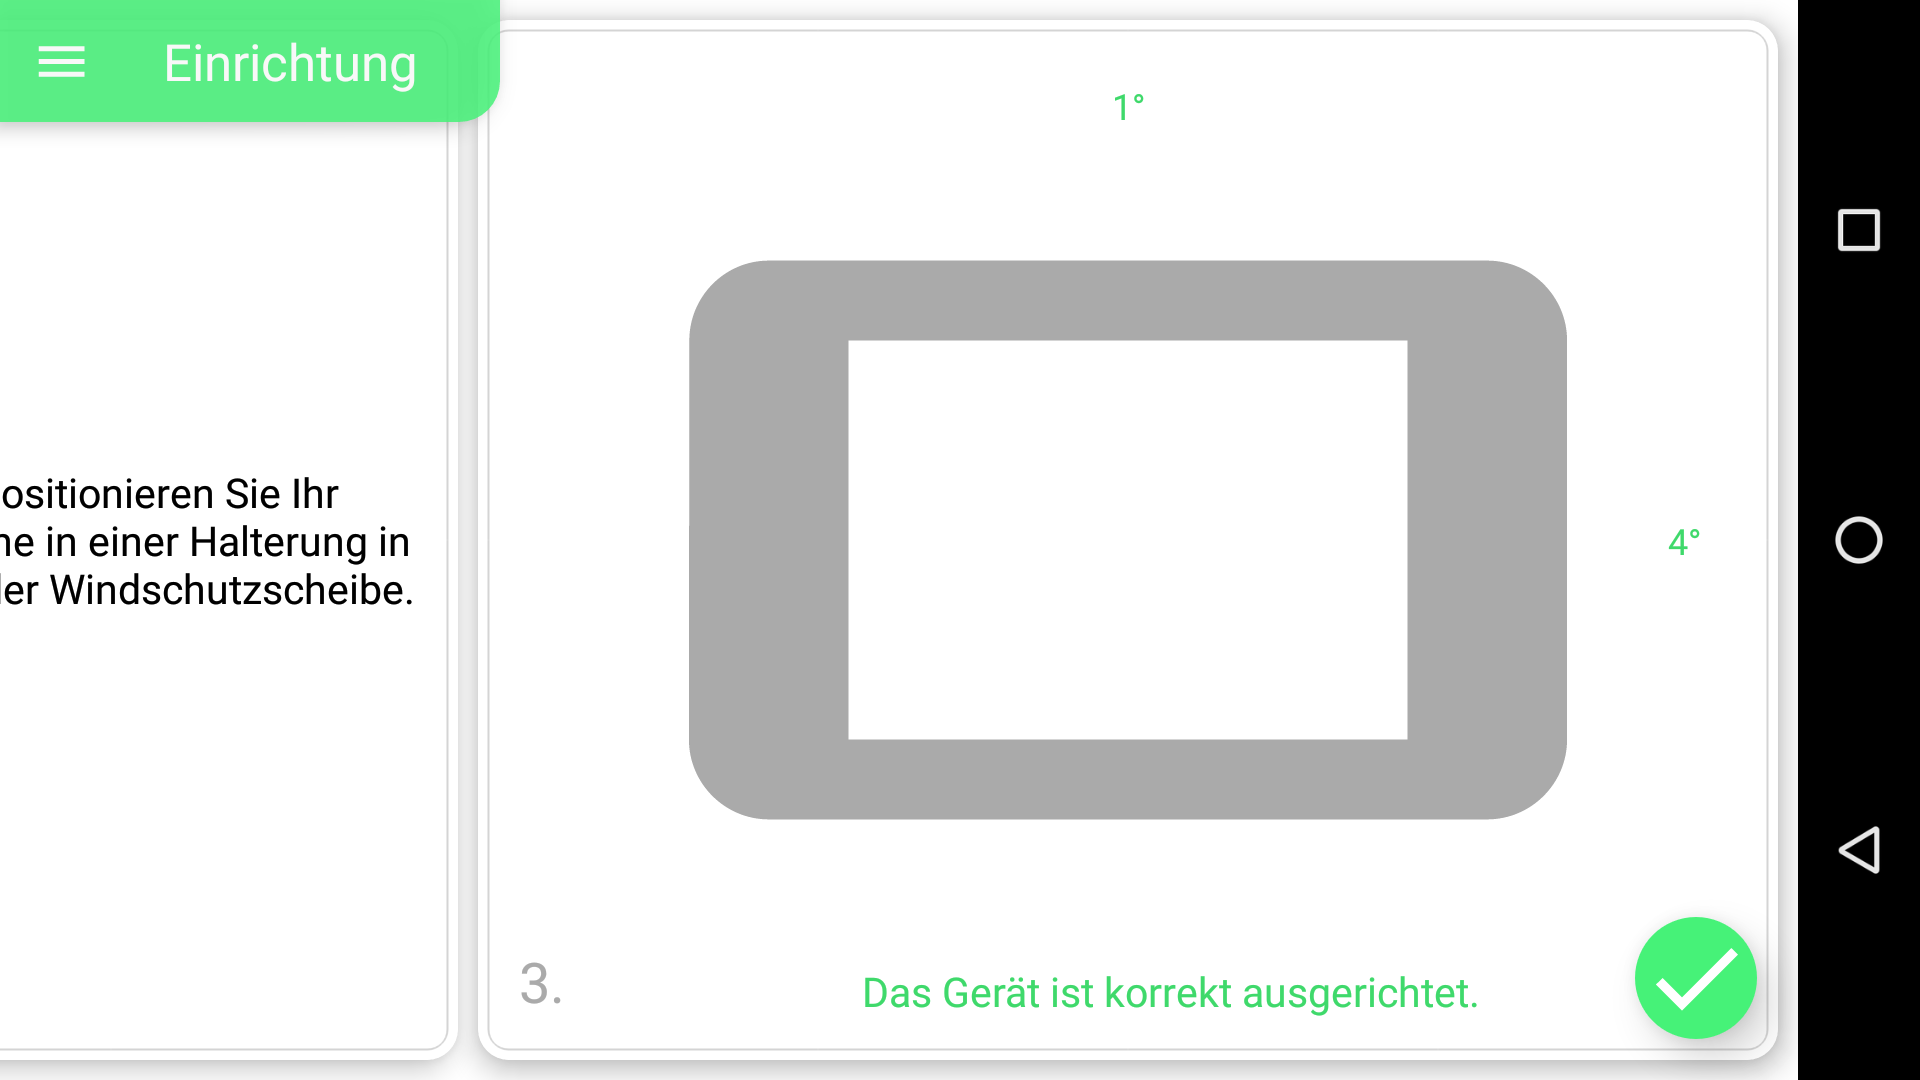
\includegraphics[width=0.9\linewidth]{Reviewdokument/Grafiken/app_setup_neu.png}
\caption{UI des Kalibrierungs-Fragmentes zu Ende der zweiten Iteration}
\end{figure}

Das Kalibrierungsmenü zeigt dem \gls{Nutzer} nun neben der \glslink{Drehachsen}{Rollachse auch die Nickachse} an. Zwar sollte es für den \gls{Nutzer} selbstverständlich sein, dass das \gls{Smartphone} mit der Kamera in Fahrtrichtung zu zeigen hat, aber es ist für Nutzer möglicherweise nicht intuitiv entscheidbar, ob es eher auf die Fahrbahn, gerade nach vorn oder in Richtung Himmel zeigen muss.\\

\section[Meilenstein 4: Filterverwaltungs-Bibliothek]{Meilenstein 4: Filterverwaltungs-Bibliothek, bis 10.06. (200 PS)}
Dieser Meilenstein umfasst neben der Implementierung der \gls{Filterverwaltungs-Bibliothek} selbst auch die Schaffung der für die Entwicklung und Ausführung derselben benötigten Voraussetzungen(Pflichtenheft P4201, P4202, P4203, P5005). Da für die Verwaltung der Neuronalen Netze TensorFlow verwendet wird und die Programmierung in C++ erfolgen sollte, war es zunächst notwendig, die entsprechenden Bibliotheken aus dem TensorFlow Quellcode zu kompilieren. Dies geschah sowohl für Android, als auch für x86-64 Linux (Ubuntu), um so ein Entwickeln auf beiden Plattformen zu ermöglichen, mit dem Ziel, die generelle Funktionsweise der \gls{API} und der \gls{Filterverwaltungs-Bibliothek} direkt aus der Entwicklungsumgebung heraus auf dem PC testen und verifizieren zu können. 
Hierbei ergaben sich einige Probleme (die mittlerweile weitgehend gelöst sind), welche im Folgenden kurz aufgelistet werden:\\

\subsubsection{Einbinden der TensorFlow Header}
Um TensorFlow mit C++ benutzen zu können, werden die entsprechenden Header mit den Deklarationen der einzelnen Funktionen, Klassen, Structs und Enumerationen benötigt. Diese sind prinzipiell auch im Quellcode von TensorFlow verfügbar. Es ist allerdings nicht dokumentiert, welche Header genau benötigt werden und wie diese den Projekteinstellungen hinzuzufügen sind: einige der Header entstehen erst, nachdem TensorFlow das erste Mal kompiliert wurde und befinden sich in gänzlich anderen Ordnern, wo diese intuitiv nicht zu vermuten wären. Es gibt allerdings auch Fälle, in denen Platzhalter für die Header in die normale Ordnerstruktur eingepflegt sind, die sich darüber hinaus oft auch noch selbst einbinden, sodass Zirkelbezüge entstehen. Die Header aus dem Quellcode und jene, welche nach dem Kompilieren entstehen, müssen dann auf eine spezielle Weise in eigene Projekte eingebunden werden. Unterordner, die bereits als Teil eines übergeordneten Ordners eingebunden wurden, müssen teilweise selbst separat als \glqq{}Include Verzeichnis\grqq{} hinzugefügt werden, da unterschiedliche Teile von TensorFlow die einzelnen Dateien unterschiedlich einbinden. Dies war allerdings nicht dokumentiert und musste durch Studieren veröffentlichter Projekte (z.B. auf GitHub) sowie ausgiebigem Experimentieren herausgefunden werden.\\

\subsubsection{Kompilieren der Librarys}
Die Bibliotheken von TensorFlow mussten sowohl für ARM-Android als auch für x86-64 Architekturen kompiliert werden. Hierbei kam es vor, dass sich die Bibliothek für einige der Architekturen, z.B. für arm64-v8a nicht erzeugen lies. Dieses Problem konnte nur durch minutiöses experimentieren, verteilt über mehrere Rechner und Distributionen, gelöst werden, da auch dies offiziell sehr wenig dokumentiert ist.\\

\subsubsection{Unterschiedliche Ops auf ARM und x86-64}
\glqq{}Ops\grqq (Operations) im Sinne von TensorFlow sind Knoten im TensorFlow Graphen, welche Berechnungen auf oder mit Tensor Objekten durchführen und selbst wieder beliebig viele Tensor Objekte zurückgeben, welche von anderen Ops benutzt werden können.
Da die zum Testen verwendete x86-64-Linux-Version anders als die ARM Version für Android kompiliert wird, kann es momentan noch zu Kompatibilitätsproblemen von verwendeten \glslink{Neuronales Netzwerk}{Neuronale Netzwerken} kommen.
Da eine lauffähige Android-Version priorisiert wird, und die Linux-Version, wie bereits angesprochen, nur zum Testen genutzt wird, liegt momentan der Fokus darauf, die richtigen Ops für Android einzubinden.\\
Jedoch wurde es geschafft, eine lauffähige Version für x86-64-Prozessoren mit AVX2 (Advanced Vector Extensions)-Support zu kompilieren. Dadurch ist ein Testen auf diesen Prozessoren möglich.\\

Während der Implementierung wurde festgestellt, dass einige, vor allem für die Detektion relevante, Ops, nicht von TensorFlow Lite unterstützt werden. Um die Funktionalität dieser Neuronalen Netzwerke zu gewährleisten, musste deswegen ein Wechsel auf TensorFlow Mobile vollzogen werden.\\
Nach dem Umstieg von TensorFlow Lite auf TensorFlow Mobile wurden wieder alle benötigten Abhängigkeiten erzeugt und eingebunden. Für die Entwicklung ist eine CMake-basierte Umgebung aufgesetzt worden. Die dynamische Bibliothek für die Android-\gls{App} wird dabei direkt aus Android Studio heraus erzeugt. Für Testzwecke wurde allerdings auch eine ndk-build Umgebung angelegt, mit derer sich der Code auch ohne Android Studio zu Testzwecken direkt kompilieren lässt.\\


\section[Meilenstein 5: Verkehrszeichen-API und Neuronale Netzwerke]{Meilenstein 5: Verkehrszeichen-API und Neuronale Netzwerke, bis 10.06. (290 PS)}
\subsection{Detektion}
Bei \glslink{Neuronales Netzwerk}{Neuronale Netzwerken} zur Objektdetektion existiert stets ein Kompromiss zwischen Geschwindigkeit und Präzision. Es gibt eine Vielzahl verschiedener Architekturen, daher ist es notwendig, die Architektur des \glslink{Neuronales Netzwerk}{Neuronalen Netzwerkes} mit Bedacht auszuwählen und diese Faktoren für das gegebene Problem optimal zu gestalten. 

Diese Geschwindigkeit kann grob bestimmt werden, indem betrachtet wird, wieviele \gls{FLOPs} die Architektur benötigt.
Hierbei ist es wichtig zu wissen, dass Smartphones mit TensorFlow Mobile aktuell nur auf \gls{CPU}, nicht auf der leistungsstärkeren \gls{GPU}, rechnen können.
Die \gls{FLOPS} von Smartphone-\gls{CPU}s ist generell eher niedrig, weswegen es absolut entscheidend ist, dass die \gls{Detektion} möglichst wenig \gls{FLOPs} benötigt um diese videotaktschritthaltend zu ermöglichen.

Jedoch ist für eine genaue \gls{Detektion} eine hohe Anzahl von \gls{FLOPs} vonnöten, um feinere Merkmale zu extrahieren. Wird die \glslink{FLOPs}{FLOP}-Zahl zugunsten der Geschwindigkeit gering gehalten, sorgt dies für eine Abnahme der Präzision.
In der folgenden Betrachtung wird der Kompromiss dargestellt.
Bei den getesteten \glslink{Neuronales Netzwerk}{Neuronalen Netzwerken} handelt es sich um auf den COCO-Datensatz\footnote{\link{http://cocodataset.org/}, 31.05.2018} trainierte, frei verfügbare Gewichte.\\
\newcounter{n}
\setcounter{n}{\value{footnote}}

\clearpage
\begin{longtabu}{|l|r|r|r|r|}
\hline
Architektur & verwendete Auflösung & geteste Laufzeit\footnotemark & \gls{FLOPs} & \gls{mAP}\footnotemark \\
\hline
Tiny YOLO v1\cite{DBLP:journals/corr/RedmonDGF15} & 448$\times$448 & 508.71 ms $\pm$ 43.35 ms & \num{4.50e9} & - \\
Tiny YOLO v2\cite{DBLP:journals/corr/RedmonF16} & 416$\times$416 & 621.04 ms $\pm$ 74.71 ms & \num{5.41e9} & 23.7\\
Tiny YOLO v3\cite{DBLP:journals/corr/abs-1804-02767} & 416$\times$416 & (nicht getestet) & \num{5.56e9} & 33.1 \\
SSDLite\cite{DBLP:journals/corr/abs-1801-04381} &300$\times$300 & 295.02 ms $\pm$ 28.05 ms & \num{1.50e9} & 22.0 \\
\hline
\end{longtabu}
\setcounter{footnote}{\value{n}}
Die verwendete Größe mAP ist ein gängiges Maß zur Bestimmung der Präzision von Objektdetektionsnetzwerken. Grundlegende Faktoren der Berechnung stellen die Abweichung der vorhergesagten Bounding Box von der gegebenen sowie die Zuordnung zur korrekten Klasse dar. Damit die Evaluierung repräsentativ ist, wird dies auf einem Teil des Datensatzes berechnet, welcher explizit nicht für das Training verwendet wurde.
Diese Tatsache ist wichtig, da das Netzwerk sonst den unfairen Vorteil hätte, die Bilder bereits gelernt zu haben. Dies würde keine zielführende Auswertung liefern, da das Netzwerk in einem realen Einsatz auch ohne spezifisch gelernte Verkehrszeichen klar kommen muss.\\
\footrealtext{Durchschnittliche Berechnungszeit auf einem \gls{Smartphone} mit Snapdragon-820-Prozessor.}
\footlinktext{http://homepages.inf.ed.ac.uk/ckiw/postscript/ijcv\_voc09.pdf}{30.05.2018}
\footlinktext{https://pjreddie.com/darknet/yolo/}{30.05.2018}


SSDLite\cite{DBLP:journals/corr/abs-1801-04381} benötigt mit Abstand von ca. 250 ms die geringste Zeit pro Eingabe und bietet dabei eine \gls{mAP}, welche der Präzision von Tiny YOLO v2\cite{DBLP:journals/corr/RedmonF16} nahe kommt und einen guten Kompromiss darstellt. Durch die deutlich geringere Rechenzeit, können mehr Frames pro Sekunde verarbeitet werden. Dadurch haben nicht oder falsch detektierte Verkehrszeichen, sofern sie in späteren Frames erneut auftauchen, eine weitere Chance korrekt detektiert zu werden.\\
Einen Nachteil bringt SSDLite\cite{DBLP:journals/corr/abs-1801-04381} mit sich, wenn es um die Auflösung geht. Ein Teil der Rechenzeit wird eingespart, indem kleinere Bilder als Eingabe für das \glslink{Neuronales Netzwerk}{Neuronale Netzwerk} verwendet wird.
Eine Auflösung von 300$\times$, erfordert, dass die Bilder noch kleiner skaliert werden als z.B. bei Tiny YoloV2\cite{DBLP:journals/corr/RedmonF16}.
Durch die Skalierung werden die Verkehrszeichen noch kleiner skaliert und sind schwieriger in dem Bild zu erkennen.\\
Es wurde sich, trotz der deutlich höheren \gls{mAP}, bewusst gegen Tiny YOLO V3\cite{DBLP:journals/corr/abs-1804-02767} entschieden.
Dies liegt daran, dass es aktuell noch keine Implementierung gibt, welche mit TensorFlow funktioniert.
Eine eigene Implementierung hätte Zeit in Anspruch genommen, weswegen auf das Testen verzichtet wurde.
Jedoch benötigt diese Architektur noch mehr FLOPs als Tiny YOLO v2\cite{DBLP:journals/corr/RedmonF16}, weswegen wir von einer leicht höheren Rechenzeit ausgehen.

Aufgrund dieser Argumente wurde sich für Verwendung von SSDLite\cite{DBLP:journals/corr/abs-1801-04381} entschieden, da es den besten Kompromiss zwischen Geschwindigkeit und Präzision für das Projekt bietet.\\
\\
Bei dem Training des \glslink{Neuronales Netzwerk}{Neuronalen Netzwerks} haben sich Probleme bemerkbar gemacht. Da der in Meilenstein 6.2. erstelle Datensatz relativ unbalanciert ist (d.h.: einige Verkehrszeichen kommen deutlich häufiger vor als andere), war es für das Netzwerk nicht möglich, die seltenen Klassen zu lernen. Um dieses Problem zu lösen, wurden so genannte \glqq{}Class Weights\grqq{} eingeführt, welche bewirken sollen, dass die selten vorkommenden Klassen mehr gelernt werden als jene, die häufigen vorkommen. Dies berücksichtigt jedoch nicht, wie gut das Netzwerk die einzelne Klasse bereits beherrscht.
Deswegen sollten die einzelnen Klassen Gewichte gut gewählt werden.
Diese Klassen Gewichte zu wählen ist jedoch erfahrungsbasiert und müsste ggf. mehrmals angepasst werden, da sonst immer noch einigen Klassen stärker gelernt werden können als andere.
%Dies hat sich auch nach erneutem Lernen durch sehr schlechte \glslink{Detektion}{Detektionsergebnisse} bemerkbar gemacht.\\
Ein weiteres Problem ist mit der eigentlichen Aufgabe des Dektektors verbunden. Dieser muss in der Lage sein, Verkehrszeichen verschiedener Klassen in einem Bild detektieren zu können. Dies ist bei Neuronalen Netzwerken nicht immer der Fall. Das verwendete Neuronalen Netzwerk ist dazu in der Lage, weil dies als Loss-Funktion 
\textit{\glqq{}Sigmoid Cross Entropy\grqq{}} benutzt, welches mit solchen \glqq{}Muitlabel\grqq{}-Problem umgehen kann. Bei einer genaueren Betrachtung der vorliegenden Probleme wurde ein Wechsel auf die Funktion \textit{\glqq{}Focal Loss\grqq{}}\cite{DBLP:journals/corr/abs-1708-02002} als sinnvoll erachtet. Diese ist eine speziell für \glslink{Detektion}{Detektionsnetzwerke} entwickelte Funktion, welche bisher schlecht gelernte Klassen, oder sogar Einzelbilder aus einer Klasse, stärker gewichtet als schon gut gelernte Beispiele.\\
Zusätzlich kann sie, wie die zuvor genutzte Loss-Funktion, auch mit \glqq{}Mutilabel\grqq{}-Problemen umgehen.
\begin{figure}[H]
\centering
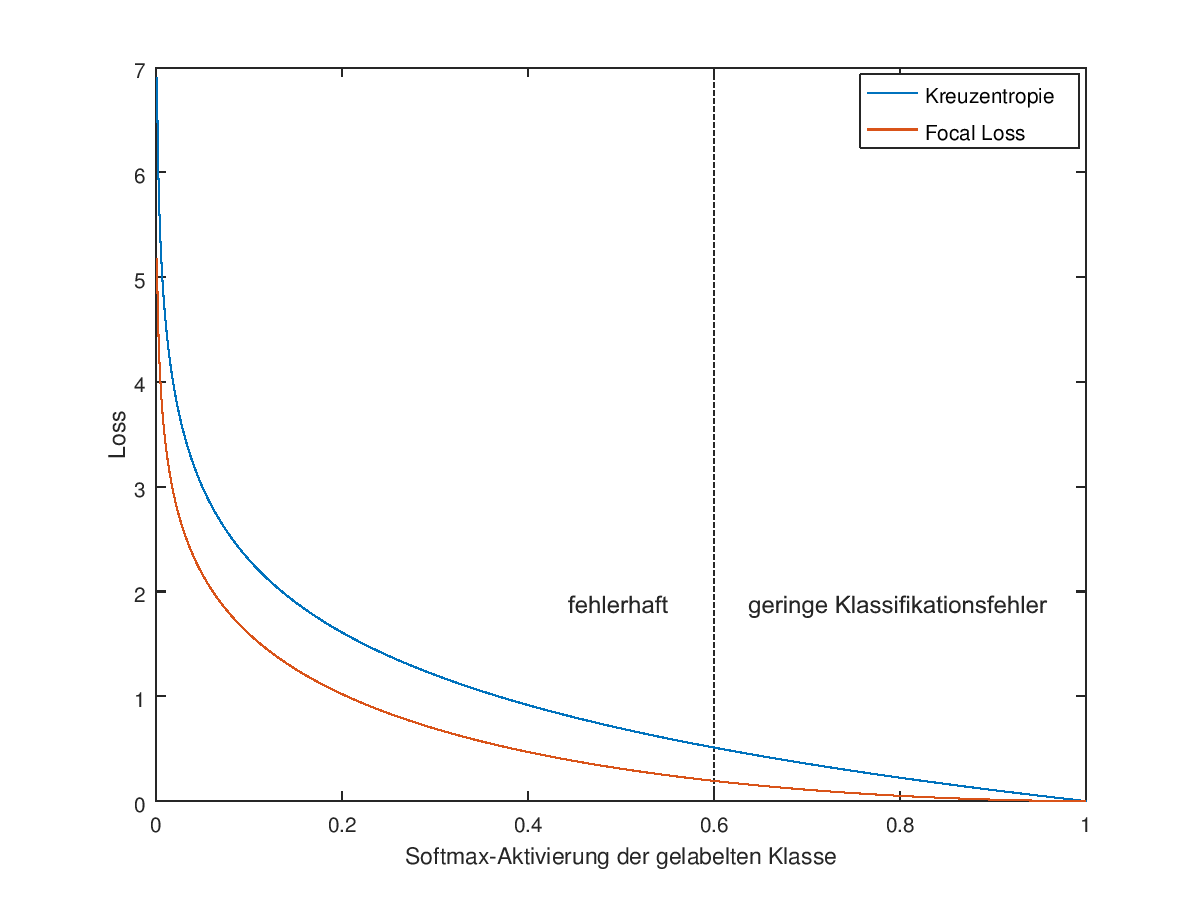
\includegraphics[width=1\linewidth]{Grafiken/lossfunktionen.png}
\caption{Vergleich der beiden Loss-Funktionen}
\end{figure}

Diese Funktion besitzt zwei einstellbare Parameter, $\alpha$ und $\gamma$, mit welchen festgelegt werden kann, wie viel stärker die schwachen \gls{Sample}s gewichtet werden. Hierbei ist es wichtig, einen guten Mittelweg zu wählen. Bei zu klein gewählten Parametern würde die Funktion die schwachen Klassen zu wenig beeinflussen. Wenn die Parameter jedoch zu groß gewählt sind, wird sogenanntes \glqq{}Overfitting\grqq{} betrieben, welches vermieden werden sollte, da dieses zu einer zu starken Spezialisierung des Neuronalen Netzwerkes führen kann.\\


Zusätzlich wurden schon bei der Detektion deutlich mehr Einzelklassen angelernt. So wurden statt den vorher verwendeten drei Klassen (geschwindigkeitsregulierende \gls{VZ}, Zusatzzeichen, sonstige \gls{VZ}) insgesamt fünfzehn Klassen(\cref{sec:klassen_detektion})
eingeführt. Vor allem die \glqq{}Sonstige Verkehrszeichen\grqq{} Klasse, welche die Mehrheit der gesamten Daten darstellte, wurde in mehrere Klassen aufgeteilt wie z.B. \glqq{}Verschiedene Gelb\grqq{}, \glqq{}Verschiedene Blau\grqq{} oder \glqq{}Verschiedene Grün\grqq{}.\\
Nach einem erneuten Training haben sich deutlich bessere \glslink{Detektion}{Detektionsergebnisse} feststellen lassen. Fast alle Verkehrszeichen wurden beim Testen erkannt. Ab und zu liegen diese jedoch noch in der falschen Klasse, was sich mit der geringen Auflösung von 300$\times$300 Pixeln in Verbindung bringen lässt. Deswegen sollte die Ausgabe der Klasse eher als \glqq{}Guess\grqq{} (Vermutung) betrachtet werden und generell nochmal in einer höheren Auflösung durch das \glslink{Klassifikation}{Klassifikatornetzwerk} ausgewertet werden.\\

\subsection{Klassifikation}
Bei \glslink{Neuronales Netzwerk}{Neuronalen Netzen} zur \gls{Klassifikation} besteht ebenfalls der Kompromiss zwischen Geschwindigkeit und Präzision. Es gibt wenige Architekturen, welche für \glslink{Smartphone}{Smartphones} ausgelegt sind: zum Beispiel MobileNetV1\cite{DBLP:journals/corr/HowardZCKWWAA17} , MobileNetV2\cite{DBLP:journals/corr/abs-1801-04381}  und NASNet-Mobile. Diese Modelle klassifizieren Bilder in sehr kurzer Zeit und haben für die Geschwindigkeit eine ausreichende Genauigkeit.\\

\begin{tabu}{|X[l]|r|r|r|}
\hline
Architektur & verwendete Auflösung & Top 1 Accuracy & CPU Laufzeit \\
\hline
MobileNetV1\cite{DBLP:journals/corr/HowardZCKWWAA17}    & 244$\times$244 & 70.6 & 113 ms \\
NasNet-A-Mobile & 244$\times$244 & 74.0 & 183 ms \\
MobileNetV2\cite{DBLP:journals/corr/abs-1801-04381}    & 244$\times$244 & 72.0 & 75 ms \\
MobileNetV2\cite{DBLP:journals/corr/abs-1801-04381}  &  96$\times$96\footnotemark[8] & 60.3 & 18 ms \\
\hline  
\end{tabu}~\\
Die Tabelle vergleicht die genannten Architekturen hinsichtlich Top 1 Accuracy und Rechenzeit. Die Top 1 Accuracy gibt an, wie viel Prozent der Netzwerkausgaben mit der höchsten Wahrscheinlichkeit mit den geforderten Ausgaben übereinstimmen. Dabei ist zu Beachten, dass die Netzwerke auf den Imagenet\footnotemark[9] Datensatz mit 1001 verschiedenen Klassen und auf der CPU eines Google Pixel 1 getestet wurden.\\

\footlinktext{https://github.com/tensorflow/models/tree/master/research/slim/nets/mobilenet}{12.06.2018}
\footlinktext{www.image-net.org/}{12.06.2018}

Beim Vergleich der genannten Architekturen unter der gleichen Auflösung der zu klassifizierenden Bilder stellte sich heraus, dass MobileNetV2\cite{DBLP:journals/corr/abs-1801-04381} eine viel kürzere Rechenzeit als NasNet-A-Mobile und eine etwas kürzere Rechenzeit als MobileNetV1\cite{DBLP:journals/corr/HowardZCKWWAA17}, wobei nur eine geringfügig schlechtere Genauigkeit als NasNet-A-Mobile und sogar eine bessere Genauigkeit als MobileNetV1\cite{DBLP:journals/corr/HowardZCKWWAA17} aufweist.
Die Geschwindigkeit der Netzwerkarchitekturen kann darüber hinaus noch gesteigert werden, wenn man eine Architektur wählt, welche für kleinere Bildgrößen konzipiert ist. 
So gibt es Netzwerkarchitekturen für kleinere Auflösungen bis hin zu 128$\times$128 für MobileNetV1\cite{DBLP:journals/corr/HowardZCKWWAA17} und 96$\times$96 für MobileNetV2\cite{DBLP:journals/corr/abs-1801-04381}.
Theoretisch würden zum Klassifizieren von Verkehrszeichen eine Bildgröße von 40$\times$40 für das menschliche Auge und somit auch für ein \glslink{Neuronales Netzwerk}{Neuronales Netzwerk} ausreichen, allerdings ist MobileNetV2\cite{DBLP:journals/corr/abs-1801-04381} in der 96$\times$96 Version das Modell mit vortrainierten Gewichten mit der kleinsten Auflösung.
Da die Klassifikation innerhalb kürzester Zeit und mit guter Genauigkeit erfolgen soll, fiel die Wahl der Architektur auf MobileNetV2\cite{DBLP:journals/corr/abs-1801-04381}.\\
Weiterhin war uns wichtig, vortrainierte Modelle zu benutzen, da diese, obwohl sie auf einen anderen Datensatz trainiert wurden, grundlegende Merkmale wie beispielsweise Kanten in einem Bild erkennen können, was den Trainingsprozess beschleunigt. Für MobileNetV2\cite{DBLP:journals/corr/abs-1801-04381} gibt es vortrainierte Modelle, welche auf den Imagenet Datensatz trainiert wurden.\\
Beim Training des Netzwerkes muss darauf geachtet werden, dass der gesammelte Datensatz nicht gut balanciert ist. Es gibt Verkehrszeichen, welche sehr häufig vertreten sind und es gibt kaum vertretene Verkehrszeichen.
Damit das \glslink{Neuronales Netzwerk}{Netzwerk} lernt, Verkehrszeichen zu klassifizieren, welche nur in geringen Mengen im Datensatz enthalten sind, kann man mit Klassen Gewichten trainieren.\\
Das \glslink{Neuronales Netzwerk}{Netzwerk} zur \gls{Klassifikation} konnte unter anderem aufgrund von fehlender Rechenleistung und Fehleinschätzung der Datensatzaufbereitung noch nicht vollständig trainiert werden, was allerdings zu Beginn der nächsten Phase nachgeholt wird.\\

\section[Meilenstein 6: App-API-Anbindung]{Meilenstein 6: App-API-Anbindung, bis 14.06. (30 PS)}
Die Smartphone Kamera kann unterschiedliche Bildformate bereitstellen. Auf allen Smartphones, welche wenigstens die API Version besitzen, die unterstützt werden soll (API Level 24, siehe Pflichtenheft) steht dabei das YUV\_420\_888 Format zur Verfügung, welches darüber hinaus auch in der offiziellen Dokumentation der Android Kamera API für Bildverarbeitung empfohlen wird. Da die von uns verwendeten Netzwerke RGB Bilder benötigen und auch nur auf solchen trainiert wurden, musste eine Konvertierung des YUV Formates in ein RGB Format erfolgen. Im Detail sei dies in \cref{sec:schnittstellendokuAPPAPI} genauer erläutert. Anschließend erfolgte die Einbindung der API relativ problemlos, zumindest nachdem die entsprechenden Tensorflow Librarys für die ARM Architektur erfolgreicht kompiliert wurden. Der Code der Filterverwaltungs-Bibliothek und Verkehrszeichen-API ist portabel, vor allem weil Tensorflow selbst weitgehend plattformunabhängig entwickelt wurde. Die bereits auf x86-64 lauffähige API wird als dynamische Bibliothek kompiliert, in die Android APP eingebunden und über die entsprechenden Funktionen des Java Native Interfaces angesprochen.\\
Resümierend lässt sich sagen, dass die angestrebten Funktionalitäten entsprechend umgesetzt wurden: die App ist in der Lage Verkehrszeichen auf von der Kamera aufgenommenen Bildern zu detektieren und zu klassifizieren (sofern die dazu benötigten Neuronalen Netzwerke bereitgestellt werden) und verwendet dafür die RoadSignAPI, welche wiederum auf der Filterverwaltungs-Bibliothek aufbaut.


\begin{figure}[H]
\centering
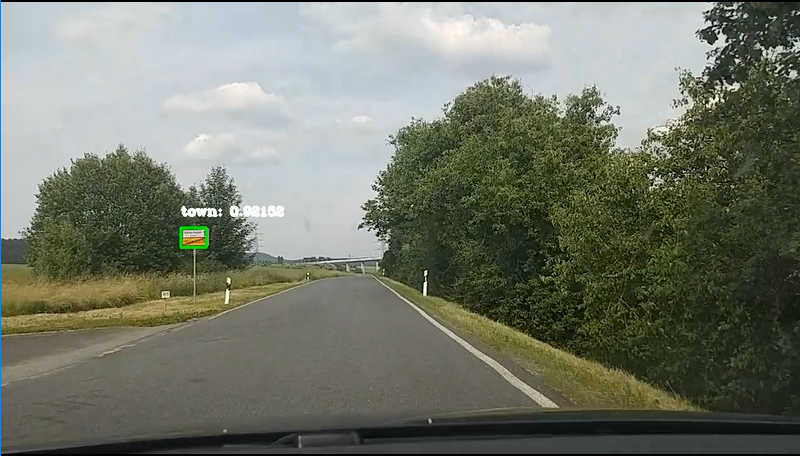
\includegraphics[width=1\linewidth]{Grafiken/detector_1.PNG}
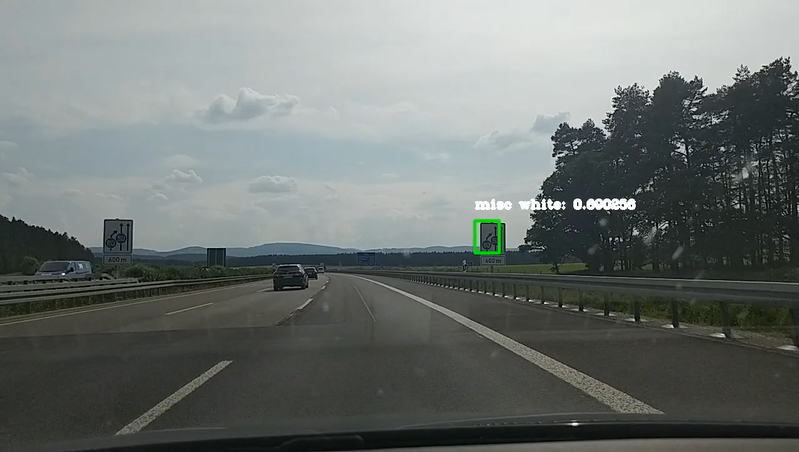
\includegraphics[width=1\linewidth]{Grafiken/detector_2.PNG}
\caption{Beispielhafte Detektion auf Testdaten}
\end{figure}

\\

\section{Ergebnisse des ersten Bug-Reviews}
\subsubsection*{Memory Leak in der \gls{App}}
Bereits während der Implementierung der \gls{App} fiel uns ein gravierender Fehler in der von Android bereitgestellten Kamera auf. Unter Android 8 \glqq{}Oreo\grqq{} kann es bei der Benutzung der Kamera zu einem Memory Leak kommen. Dies ist ein Fehler, auf welchen man als \gls{App}-Entwickler ohne Weiteres keinen Einfluss hat.\\
Es wurde versucht, das Memory Leak dadurch einzudämmen, dass periodisch der Java-Garbage-Collector aufgerufen wird. In dem \glqq{}richtigen\grqq{} Bug-Review in der dritten Phase wird dies weiter untersucht, sofern ein Memory Leak in der \gls{App} Probleme macht.\\

\subsubsection*{Deadlock in der \gls{App}}
Für das Starten und Beenden der Smartphone-Kamera existiert ein Semaphor, das heißt, dass vor dem Öffnen der Kamera der Semaphor reserviert wird und wieder freigegeben würde, sobald die Kamera geöffnet ist. Derselbe Semaphor wird auch zum Schließen der Kamera benutzt, da die Kamera nicht gleichzeitig gestartet und beendet werden darf. Der Bug bestand darin, dass die Berechtigungen für die Kamera angefragt wurden, nach dem der Semaphor reserviert wurde, aber bevor er wieder freigegeben wurde. Wenn die Berechtigung für die Kamera angefragt wird, wird dem Nutzer ein Dialogfenster angezeigt und die Aktivität pausiert; allerdings wird beim Pausieren der Aktivität auch versucht, die ggf. geöffnete Kamera wieder zu schließen. Die App würde jetzt versuchen, den Semaphor zum Starten/Beenden der Kamera zu bekommen, welcher aber bereits dadurch reserviert war, dass die Kamera noch nicht vollständig geöffnet wurde. Dies führte zu einem Deadlock in der App und zum Einfrieren derselben.\\

\begin{figure}[H]
\centering
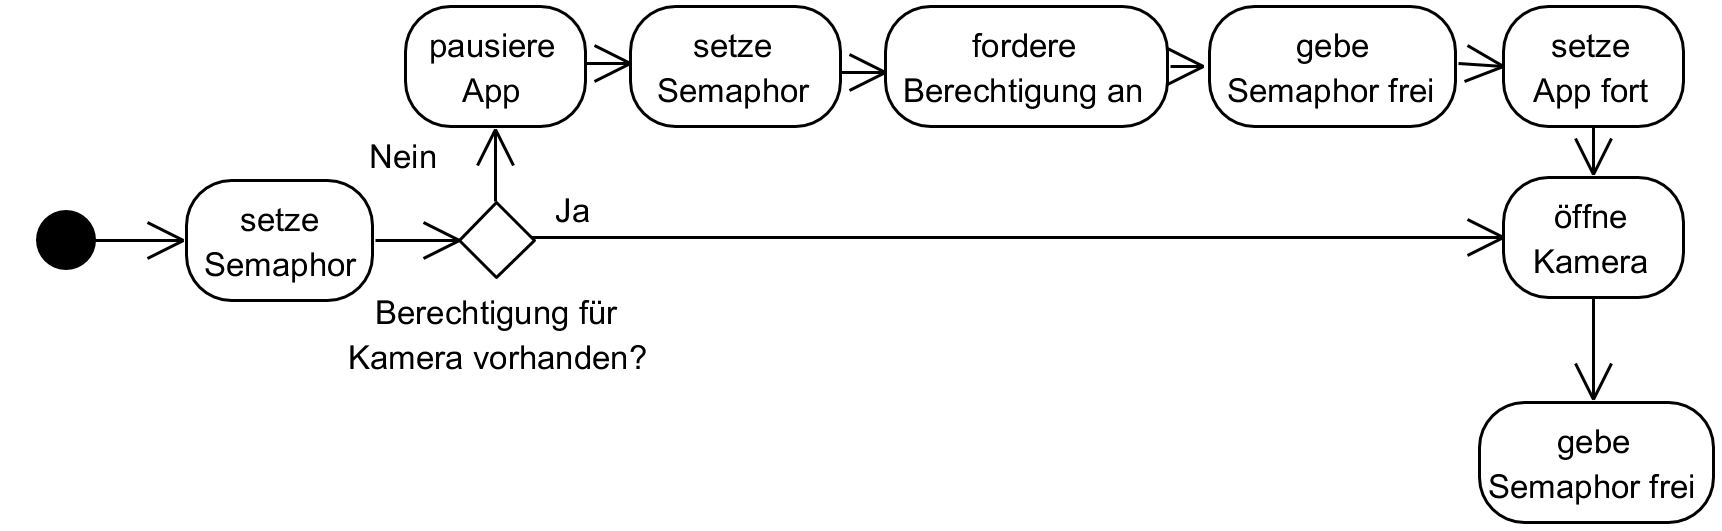
\includegraphics[width=1\linewidth]{Reviewdokument/Grafiken/app_deadlock.png}
\caption{Bei dem Versuch, den Semaphor ein zweites Mal zu setzen, tritt der Deadlock ein.}
\end{figure}

Dieser Deadlock wurde dadurch korrigiert, dass nun zuerst die Berechtigung für die Kamera angefragt und der Semaphor erst dann reserviert wird, wenn die Berechtigungen auch vom Nutzer gewährt wurden.\\

\section{Festlegung der Aufgaben für die dritte Iteration}
In der dritten und letzten Iteration sollen einige Kleinigkeiten, für die sich in der Implementierungsphase keine Zeit gefunden hat, umgesetzt werden. Hauptaugenmerk der dritten Iteration soll allerdings auf dem Systemtest liegen, welcher im Projektplan auf einen Zeitaufwand von 60 Personenstunden, also 480 h, angesetzt wurde.\\
Das \glslink{Neuronales Netzwerk}{Neuronale Netzwerk} zur \gls{Klassifikation} soll trainiert werden. Des Weiteren sind die 
\glslink{Neuronales Netzwerk}{Neuronalen Netzwerke} auf Fehldetektionen und -klassifikationen zu untersuchen. Sie bezeichnen den Fall, wenn Ausgaben vom Netzwerk falsche Ergebnisse beinhalten.
Das kann z.B. eine falsche Detektion oder eine falsche Klassifikation sein, aber auch ein nicht-Erkennen von tatsächlich vorhandenen Verkehrszeichen.
Dies ist wichtig zu untersuchen, da die Auswirkungen für unser Problem der Verkehrszeichenerkennung relevant sind und ggf. ein Nachtrainieren der Netzwerke stattfinden muss.\\
Ferner soll das \gls{Tracking} in Betracht gezogen werden. Es wurden in der zweiten Iteration bereits Versuche dahingehend unternommen, sodass die Erfolgswahrscheinlichkeit relativ hoch ist.\\

\chapter{Verifikation der abgeschlossenen Meilensteine}
Es wurden für jeden der Meilensteine auch Testkriterien festgelegt. Da diese im Reviewdokument aus Phase I fehlen, werden sie hier nachgereicht.\\
In diesem Abschnitt soll es um die Überprüfung dieser gehen, wobei insbesondere auf die dort angesetzten Testfälle eingegangen wird. \\

\section{Meilenstein 1: App-Prototyp}
\textbf{Testkriterium}: Der Prototyp lässt sich auf einem Android-Smartphone starten. Die bis hierhin implementierten Realisierungen der Benutzeroberfläche, sollten vom Prinzip her mit der Spezifikation im Pflichtenheft übereinstimmen. Des Weiteren muss eine Einbindung von TesorFlow Lite funktionieren, was durch ein Laden der Bibliothek getestet wird.\\
\\
Der App-Prototyp stand bereits zu Ende der ersten Phase und sah dem im Pflichtenheft spezifizierten \gls{UI} sehr ähnlich. Der Meilenstein wurde dadurch überprüft, dass der Prototyp auf einem Android Smartphone läuft und die \gls{UI} mit der aus dem Pflichtenheft(Abb. 6.1) zu vergleichen ist. Zusätzlich wurde die Einbindung von TensorFlow Lite sichergestellt, indem die Bibliothek geladen wurde.
Zu diesem Zeitpunkt war noch nicht bekannt, dass es Probleme mit TensorFlow Lite bezüglich der Anwendung der Netzwerke geben wird. Später wurde ein Wechsel auf TensorFlow Mobile vollzogen, was in diesem Meilenstein jedoch noch nicht berücksichtigt werden konnte.\\
Somit gilt, trotz der späteren Probleme mit TensorFlow Lite, der Meilenstein als erreicht.\\

\section{Meilenstein 2: Aufnahme und Labeln aller Samples}
\textbf{Testkriterium}: Es wird eine gegenseitige stichprobenartige Kontrolle durchgeführt, in welcher überprüft wird, ob Verkehrszeichen mit den richtigen Labels versehen wurde und ob die Verkehrszeichen gut im Bild markiert sind. Dadurch fallen Unterschiede bei der Qualität des Labelings auf. Der Meilenstein ist erst dann abgeschlossen, wenn die Samples in einer zum Training verwendbaren Qualität und Quantität vorhanden sind.\\ 
\\
Die aufgenommenen und \glslink{Label}{gelabelten} \gls{Sample}s wurden stichprobenartig überprüft und die dabei gefundenen Fehler wurden entsprechend korrigiert. Daraufhin folgend wurden die Samples mithilfe verschiedener Python-Skripte in ein zum Training geeignetes Format gebracht.\\

\begin{longtabu}{|X[l]|r|r|}
    \hline
    Verkehrszeichenart & geforderte Samplezahl & erzeugte Samplezahl\\
    \hline
    Geschwindigkeitsregulierend & 1500 & 5365 \\
    \hline
    Zusatzzeichen & 1500 & 3320 \\
    \hline
\end{longtabu}

Die im Review Dokument aus der ersten Phase spezifizierten Anforderungen bezüglich der zu erreichende Samplezahl wurden erfüllt. Jedoch muss einschränkt dazu gesagt werden, dass durch eine Herunterskalierung für das Detektions Netzwerk mit deutlich weniger Verkehrszeichen zu rechnen ist. Dort müssen bereits gelabelte Verkehrszeichen evtl. verworfen werden, da diese durch die Skalierung zu klein werden. Für die Klassifikation ist dieser Datensatz jedoch voll verwendbar.\\
Da die Kriterien des Meilensteins erfüllt wurden, gilt dieser als erfüllt.\\

%Da die Samples nun in einem Format vorlagen, welches zum Training verwendet werden kann, wurde dort per manueller Überprüfung, welche von Skripten unterstützt wurde, festgestellt, dass die Qualität der erwarteten entspricht. Somit gilt der Meilenstein als abgeschlossen.\\
%Die Daten wurden bereits erfolgreich zum Training verwendet, von daher ist auch davon auszugehen, dass die Qualität und Quantität hinreichend gut war.\\

\section{Meilenstein 3: App}
\textbf{Testkriterium}: Die Benutzeroberfläche der App ist eine ggf. leicht veränderte Version der Oberfläche aus Meilenstein 1. Das \gls{UI} soll in deutscher und englischer Sprache verfügbar sein, wobei Englisch die Fallback-Sprache darstellt. Letzteres ist mit einem \gls{Smartphone}, bei welchem nicht Deutsch als Gerätesprache eingestellt ist, zu testen. Beim Start der \gls{App} kann auch der geforderte Disclaimer überpüft werden.\\
Die Geschwindigkeitsmessung wird in einer Testfahrt mit dem Fahrzeugtachometer verglichen. Grundsätzlich sollten diese übereinstimmen, jedoch ist bei konstanter Geschwindigkeit des Fahrzeuges eine Abweichung um $\pm 5\%$ vom Tachometer akzeptabel.\\
Zum Überprüfen der Kamerafunktionalität muss in einem Debug-Menü das Bild ohne signifikanten Zeitunterschied\footnote{d.h.: der Zeitunterschied würde die Funktion des Gesamtsystems nicht beeinträchtigen} erkennbar sein.\\
Im Kalibrierungsmenü muss die Rotation des \gls{Smartphone}s zumindest als Textausgabe angezeigt werden. Bestätigt wird dies durch Drehen um $\pm90^\circ$ um die \glslink{Drehachsen}{Roll- und Nickachse} von der Nulllage (Gerät hängt waagerecht) aus.\\
Die Anforderungen, dass die Geschwindigkeitsermittlung abschaltbar sein soll und dass die Länge der Historie einstellbar ist, wird überprüft, indem diese Einstellungen im entsprechenden Menü vorgenommen werden. \\
\\
Das \gls{UI} wurde in einer direkten Sichtkontrolle überprüft (vgl. Plichtenheft Abb. 6.1).
Die aktuelle Verkehrszeichenkombination wird immer dargestelt (Pflichtenheft B6001).
Eine Zeitliche Historie in der App ist vorhanden (Pflichtenheft P4302) und die Anzahl der maximalen Elemente, welche in der Historie gespeichert werden, lässt sich auch individuell konfigurieren (Pflichtenheft P4303).
Wie gefordert, wird einer durch eine Wischgeste veränderlicher Ausschnitt der Historie, dargestellt (Pflichtenheft B6002). Zu jedem Element aus der Historie ist der Zeitpunkt der Erkennung ersichtlich (Pflichtenheft B6003). Die implementierte Geschwindigkeitsmessung (Pflichtenheft P4304) wurde in einer Testfahrt überprüft, wobei der Beifahrer das Tachometer mit der in der \gls{App} angezeigten Geschwindigkeit verglichen hat. Während die erste Implementierung (direkte Berechnung noch gelegentlich Ausreißer besaß, ist die Implementierung mit Ringspeicher hinreichend genau und zeigt bei Fahrt mit konstanter Geschwindigkeit auch eine konstante Geschwindigkeit an.\\
Auch das Ausschalten der Geschwindigkeitsmessung funktioniert wie erwartet (Pflichtenheft P4305 und B6009) und kann bei einer Überschreitung auch visuell warnen (Pflichtenheft B6004).
Das Kalibrierungsmenü (Pflichtenheft P4306) wurde getestet, indem das \gls{Smartphone} aus der Nulllage (Gerät hängt waagerecht) in beide Richtungen gedreht wurde. Bei Übertretung der zugelassenen größten Neigung zeigt das Kalibrierungsmenü richtigerweise dem \gls{Nutzer} einen Hinweis an.\\
In dem Debug-Menü wurde das Kamerabild angezeigt und für gut befunden. Die Qualität des von der Kamera bereitgestellten Bildflusses ist gut genug, um darauf die Detektions- und Klassifikationsnetzwerke anzuwenden. Dies kann allerdings erst dann vollständig verifiziert werden, wenn wir auch sichergehen können, dass unsere Annahme richtig ist. Dies sollte in Meilenstein 6 der Fall sein.\\
Der Disclaimer (Pflichtenheft P4307) wurde als Dialog\footnote{\link{https://developer.android.com/guide/topics/ui/dialogs}, 10.06.2018} beim Start der \gls{App} realisiert.\\
Die Übersetzung in beliebige Sprachen (Pflichtenheft 1.4 zweites Sollkriterium) ist durch den in Android Studio integrierten Translation Editor sehr einfach handhabbar. Es existiert momentan eine englische und eine deutsche Sprachlokalisierung, wobei Englisch als Standard-Sprache gewählt wurde (Pflichtenheft B6008).
Insgesamt läuft die App nur, wie gefordert, im Querformat (Pflichtenheft B6007).\\
Alle Musskriterien des Meilensteins wurden erfüllt uns ließen sich auch entsprechend bestätigen, wodurch der Meilenstein als erfüllt gilt.\\

\section{Meilenstein 4: Filterverwaltungs-Bibliothek}
\textbf{Testkriterium}: Im Allgemeinen lassen sich beliebige Filter anlegen (die Implementierung der internen Verarbeitungslogik, also der Operationen die der Filter ausüfhren soll, obliegt dabei dem Anwender) und einer Pipeline hinzufügen. Die Pipeline kann den Filter verwenden, um eine bestimmte Aufgabe zu lösen. Konkret lässt sich ein Filter anlegen, welcher ein beliebiges, in TensorFlow trainiertes \gls{Neuronales Netzwerk}, lädt. Zusätzlich soll man einen Input geben und die zum Output verstrichene Zeit messen können.\\
\\
Es wurde ein Filter erstellt, welcher ein vortrainiertes MobileNetv2 Netzwerk geladen hat. Dort wurde ein Beispiel-Bild mit bekannter Ausgabe in das Netzwerk reingegeben. Dabei entsprach die Ausgabe der Erwartung. Zusätzlich wurde die Laufzeit gemessen. \\
Weiterhin wurde zu Testzwecken ein vortainiertes \glqq{}Tiny YoloV2\grqq{}\cite{DBLP:journals/corr/RedmonF16} Netzwerk geladen, wodurch die in 2.4 diskutierten Probleme offenbart und wie dort bereits angesprochen gelöst wurden.\\

Desweitern wurde ein Filter angelegt, welcher ein Bild skalieren kann.
Somit lassen sich beliebige Filter anlegen (Pflichtenheft P4201 und P4202).
Da die Testkriterien erfüllt wurden, gilt der Meilenstein als abgeschlossen.\\

\section{Meilenstein 5: Verkehrszeichen-API und Neuronale Netzwerke}
\textbf{Testkriterium}: Die \gls{Verkehrszeichen-API} kann sowohl das Detektion- als auch den Klassifikationsfilter anlegen. Dort sollte ein Testbild aus dem Datensatz geladen und ausgewertet werden können. Dieses Testbild darf nicht zum Training der Neuronalen Netzwerke verwendet werden. Wenn auf dem Testbild die geschwindigkeitsregulierenden Verkehrszeichen detektiert und klassifiziert wurden, gilt der Meilenstein als abgeschlossen.\\
\\
Sowohl das Detektionsnetzwerk als auch das Klassifikatornetzwerk wurden als Filter, verbunden über eine Pipe, angelegt. Danach wurde ein Testbild, welches nicht zum Training verwendet wurde, der Pipeline übergeben(Pflichtenheft P4203). Die \gls{Verkehrszeichen-API} war wie gefordert in der Lage, mithilfe des Detektionsnetzwerkes das vorliegende Verkehrszeichen zu lokalisieren (bedingte Erfüllung aus Pflichtenheft von P4101). Außerdem lässt sich die Anzahl der echt parallelen Threads einstellen. (P4204)
Beim Testen des Detektionsnetzwerks, konnte keine Fehldetektion (False Positive) von geschwindigkeitsbegrenzenden Verkehrszeichen festgestellt werden (Pflichtenheft P4102). Dies kann an der geringen Inputgröße des Netzwerk liegen, muss jedoch in der dritten Phase noch weiter untersucht werden.\\
Die Klassifikation, wurde wie bereits in 2.5 beschrieben nicht vollständig erfüllt, wodurch der Meilenstein noch nicht als erreicht gilt.
Dies muss schnellst möglich nachgeholt werden.\\

\section{Meilenstein 6: App-API-Anbindung}
\textbf{Testkriterium}: Die \gls{App} ist in der Lage, das Kamerabild an die Filterverwaltungs-Bibliothek weiterzugeben.
Diese muss dann mithilfe der Verkerszeichen-API eine Auswertung des Bildes vornehmen.\\\\
Die Anbindung gilt als abgeschlossen, sobald die eigens trainierten \glslink{Neuronales Netzwerk}{Neuronalen Netze} mittels der Verkehrszeichen-API in der \gls{App} verwendet werden können.
Dies wird getestet, indem die Kamera eines \gls{Smartphone} auf ein Verkehrszeichen ausgerichtet wird. Dabei sind außerdem Ausgaben in Form von Statusinformationen von der \gls{Filterverwaltungs-Bibliothek} in der Konsole zu erwarten.\\
Trotz der leicht unvollständigen Erfüllung des fünften Meilensteins (Klassifikatornetzwerk liefert noch eine zu Vorhersage), wurde parallel mit der App-API-Anbindung fortgefahren.
Dies hat soweit geklappt und es wurde bereits ein Verkehrszeichen per Kamera aufgenommen und mithilfe der Filterverwaltungs-Bibliothek in Kombination mit der Verkehrszeichen-API auch entsprechend detektiert. Dies bestätigt, dass die Annahme der Kameraqualität aus Milestone 4 korrekt war. Damit ist die eigentliche Anbindung abgeschlossen, obwohl Meilenstein 5 nicht erreicht wurde.
Der Meilenstein gilt trotzdem als erreicht, da die bevorstehenden Änderungen an besagtem Meilenstein keine neuen Probleme hervorrufen kann.
Somit gilt der Meilenstein dennoch als abgeschlossen.
\\

\part{Grobentwurf}
\chapter{Entwurfsziele}
Viele Oberklasse-Fahrzeuge verfügen bereits über ein System, welches mit der eingebauten Kamera im Innenspiegel die vorausliegenden Verkehrszeichen erkennen kann. Für viele ältere bzw. preisgünstigere Fahrzeuge gibt es bisher keine rentable Möglichkeit, ein solches \gls{System} nachzurüsten. Das Ziel dieses Softwareprojektes ist die Entwicklung einer Software, welche in jedem PKW mittels geeignetem \gls{Smartphone} die Nachrüstung eines solchen \glslink{System}{Systems} ermöglicht.\\
Obwohl wir das möglichst genaue Einhalten des Entwurfes anstreben werden, liegt es natürlich im Bereich des Möglichen, dass das endgültige \gls{Produkt} in mehrerlei Hinsicht geringfügig oder stark vom ursprünglichen Entwurf abweichen kann. Insbesondere im Bereich der Neuroinformatik sind Architekturmuster oft sehr kurzlebig, aber auch bei der \gls{App} ist nicht zu garantieren, dass sich das \gls{Produkt} auch genau an den Entwurf halten wird. Obwohl eine möglichst geringe Kopplung angestrebt wird, ist es nicht auszuschließen, dass eine grundlegende Änderung in einem Subsystem auch Änderungen in den anderen Subsystemen zur Folge haben kann.\\

\section{Portierbarkeit}
Im Sinne des Hauptzieles des Softwareprojektes, die Nachrüstbarkeit auf ältere und preisgünstigere Fahrzeuge, spielt es eine tragende Rolle, die Funktionalität der Verkehrszeichenerkennung auch auf andere Systeme übertragen zu können. Die \gls{App} wird zwar nur für Android programmiert, aber es soll problemlos möglich sein, mit derselben \gls{API} auch eine \gls{App} für Endgeräte mit anderen Betriebssystemen zu programmieren.\\

\section{Korrektheit} Das \gls{System} soll die Verkehrszeichen selbstverständlich richtig erkennen.\\

\section{Zuverlässigkeit} Zuverlässigkeit spielt insbesondere für die portierbare \gls{API} eine große Rolle, aber auch die \gls{App} soll möglichst selten Betriebsstörungen aufzeigen.\\

\section{Benutzerfreundlichkeit} Die \gls{App} soll intuitiv bedienbar sein und auch unerfahrenen \glslink{Nutzer}{Nutzern} eine möglichst einfache Interaktion mit dem \gls{System} ermöglichen.\\

\section{Performanz} Damit die Verkehrszeichenerkennung im realen Betrieb auch sinnvoll funktioniert, darf zwischen Vorbeifahrt am Verkehrszeichen und Anzeige auf dem Bildschirm maximal eine Sekunde vergehen. Sowohl \gls{App} als auch \gls{API} sind für die Performanz verantwortlich.\\

\chapter{Geplanter Entwurf}
Der Entwurf aus dem Endwurfsdokument wurde nicht abgeändert, da während der
Implementierungsphase keine Abweichungen oder Änderungen hinsichtlich des Grobentwurfes nötig waren. Der geplante Kontrollfluss sowie die festgelegte Subsystemstruktur konnten die Entwurfsziele soweit erfüllen.
\section{Systemzerlegung}

\begin{figure}[H]
\centering
\includesvg[width=1\linewidth]{Grafiken/Component_Diagram.svg}
\caption{Subsystemstruktur}
\end{figure}
\label{sec:subsystemstruktur}

Die Funktionalität der Verkehrszeichenerkennung wird aus der \gls{App} ausgelagert. Das Ziel ist dabei, diese Funktionalität möglichst modular zu gestalten, damit sie auf verschiedenen Endgeräten mit verschiedenen Betriebssystemen zum Einsatz kommen kann, während die \gls{App} ausschließlich für Android vorgesehen ist. Dabei wird das \gls{System} in zwei Subsysteme zerlegt - Front End und Back End. Das Front End wird von der \gls{App} realisiert und stellt lediglich die Benutzeroberfläche zur Verfügung. Das Back End besteht aus der \gls{Verkehrszeichen-API}, welche ihrerseits auf die  \gls{Filterverwaltungs-Bibliothek}  zugreift. 

Die \gls{App} greift, wenn sie ein Verkehrszeichen erkennen soll, auf die \gls{Verkehrszeichen-API} zu, welche die einzige Schnittstelle darstellt, die die \gls{App} zu den \glslink{Detektion}{Detektions}- und Klassifizierungsnetzen hat. Die \gls{Verkehrszeichen-API} ist ferner eine Spezialisierung der zugrunde liegenden  \gls{Filterverwaltungs-Bibliothek} , wobei diese auch, durch entsprechende Konfiguration, für andere \glslink{Detektion}{Detektionsprobleme} als bloß zur Verkehrszeichenerkennung verwendet werden kann. Das Ziel dabei ist es, die Schnittstelle zwischen \gls{App} und \gls{API}s möglichst einfach zu halten und das gesamte zugrundeliegende Netzwerk soweit wie möglich zu abstrahieren. Aus Sicht der \gls{App} existiert keine  \gls{Filterverwaltungs-Bibliothek} . Die \gls{App} \glqq{}sieht\grqq{} nur die \gls{Verkehrszeichen-API} als Black Box.\\

\subsection{Kontrollfluss}
\begin{figure}[H]
\centering
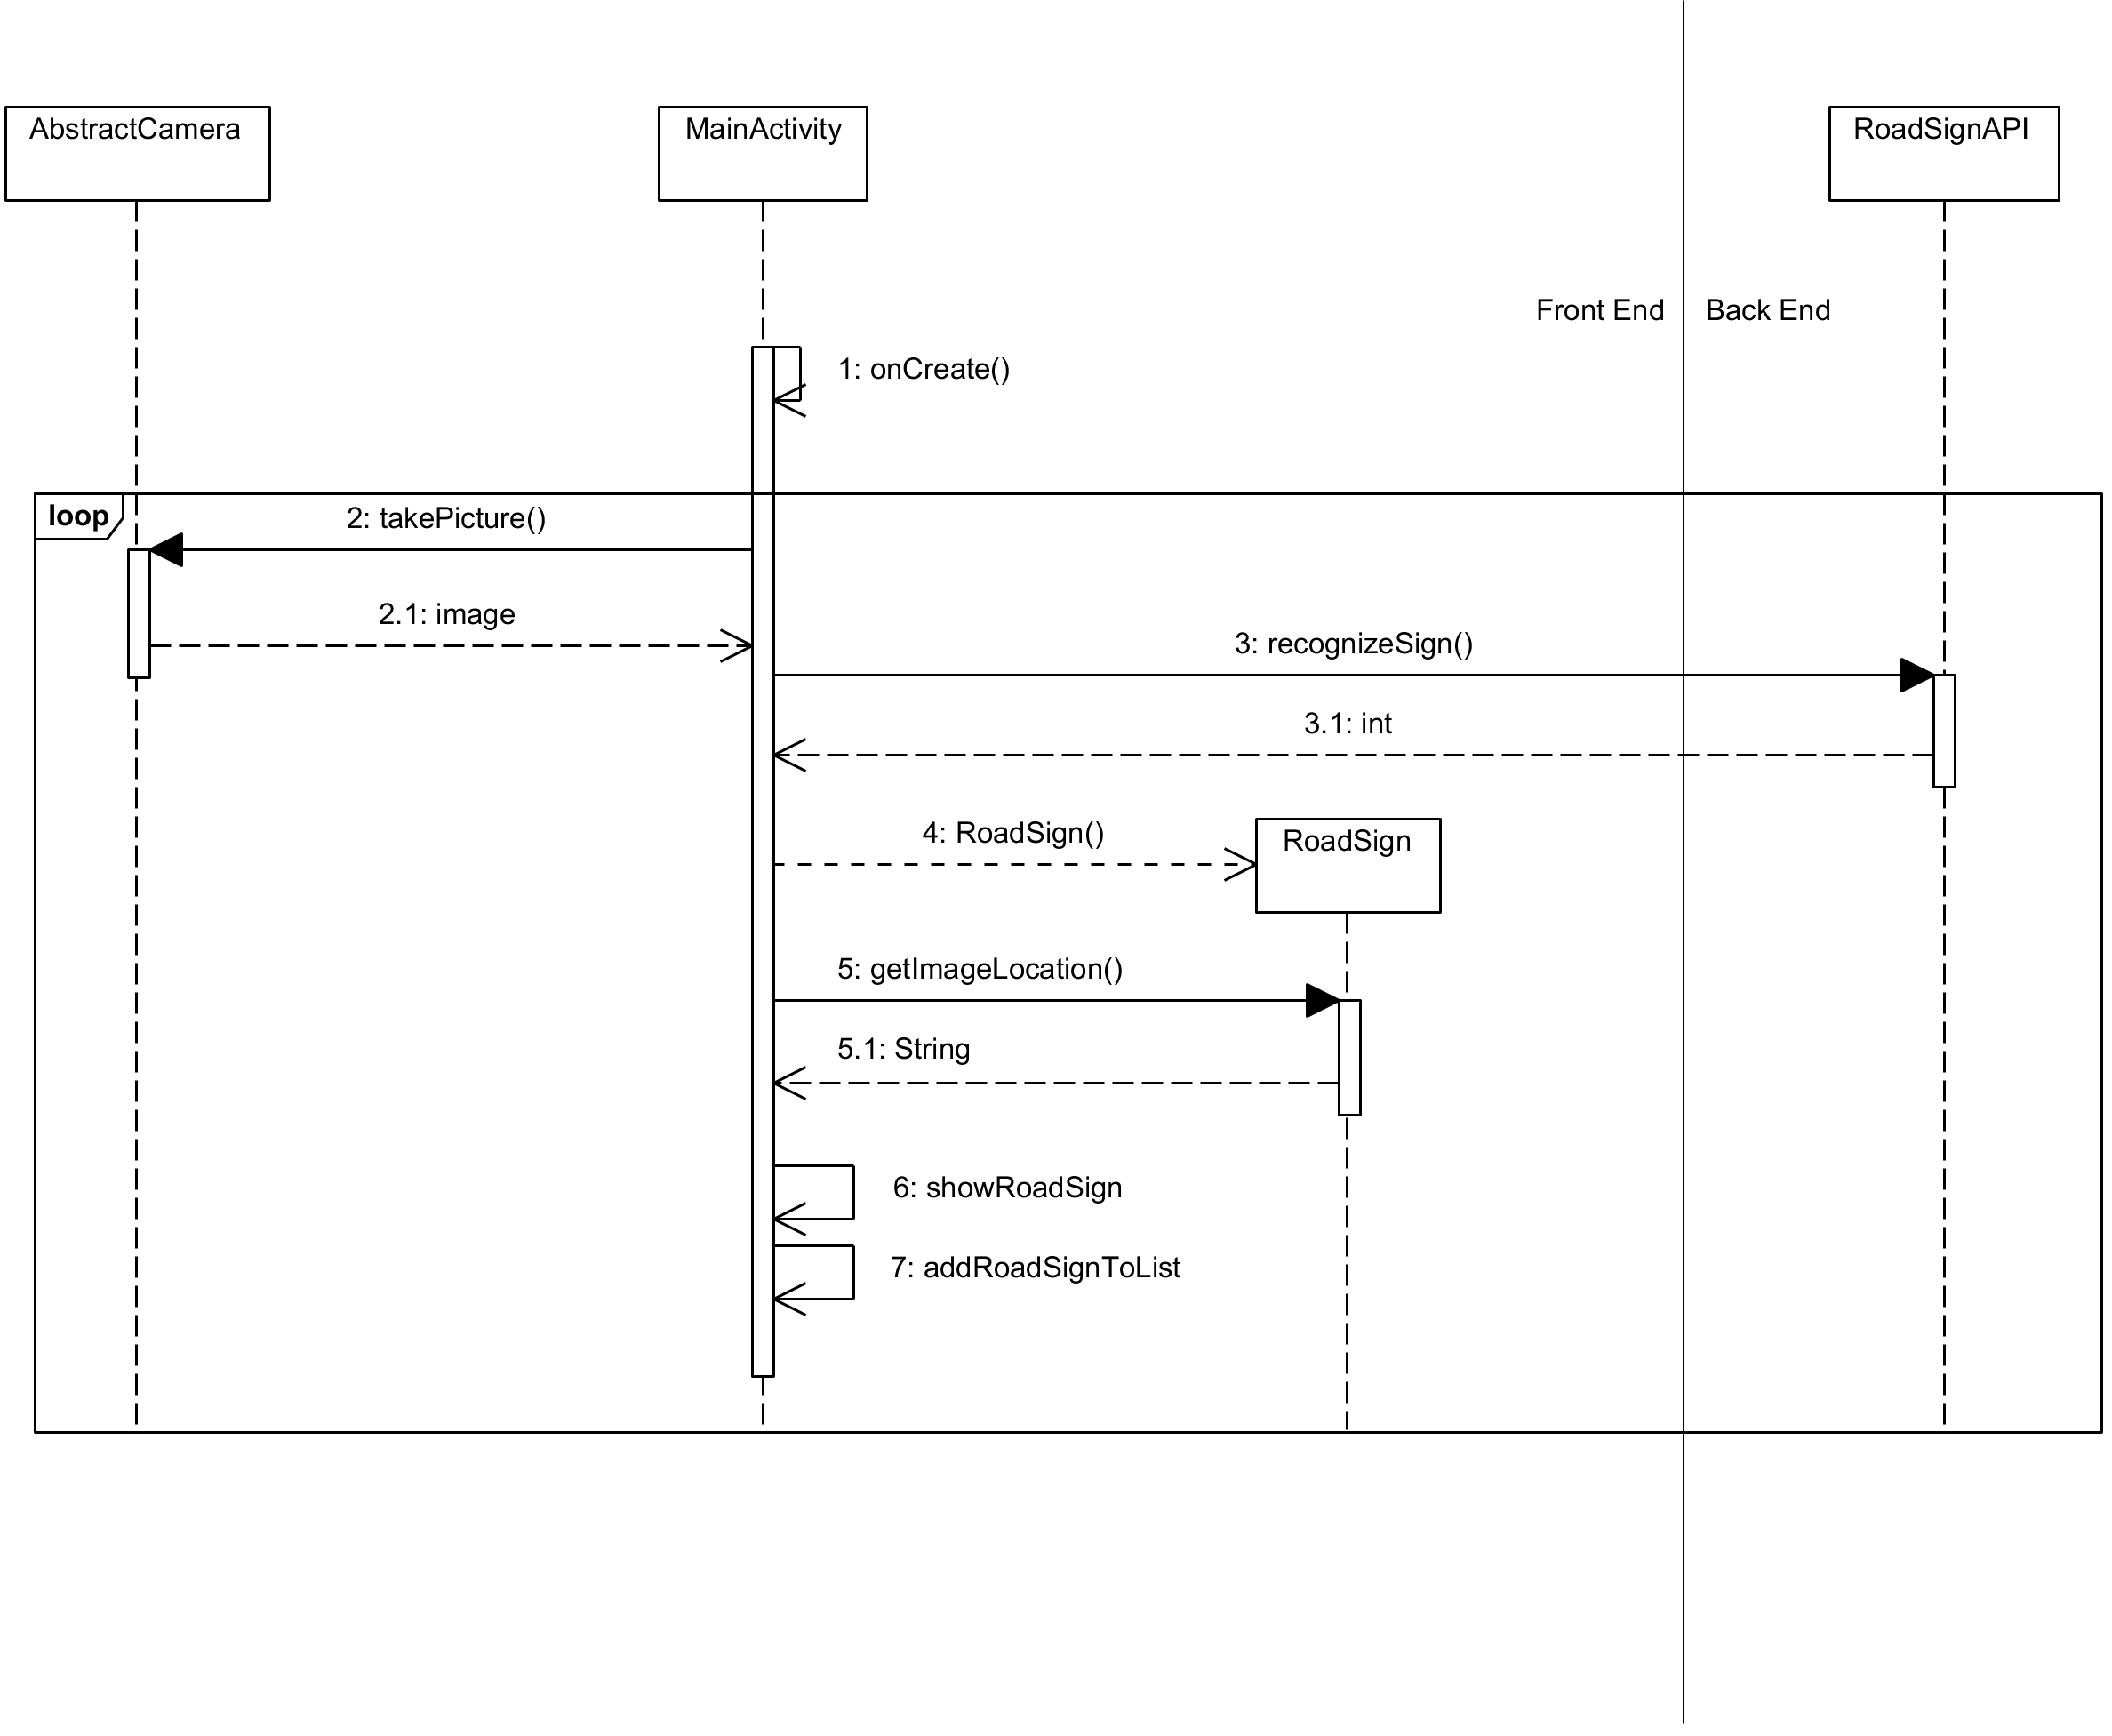
\includegraphics[width=0.9\linewidth]{Reviewdokument/Grafiken/Sequence_Diagram.png}
\caption{Erkennung eines Verkehrszeichens aus Sicht der App}
\end{figure}

Das Sequenzdiagramm aus Abb. 5.2 zeigt nochmals die geringe Kopplung zwischen den Subsystemen \gls{App} und \gls{API}. Die Kommunikation zwischen Front End und Back End erfolgt hier nur über eine einzige Funktion.\\
\label{subsec:kontrollfluss}

\begin{figure}[H]
\centering
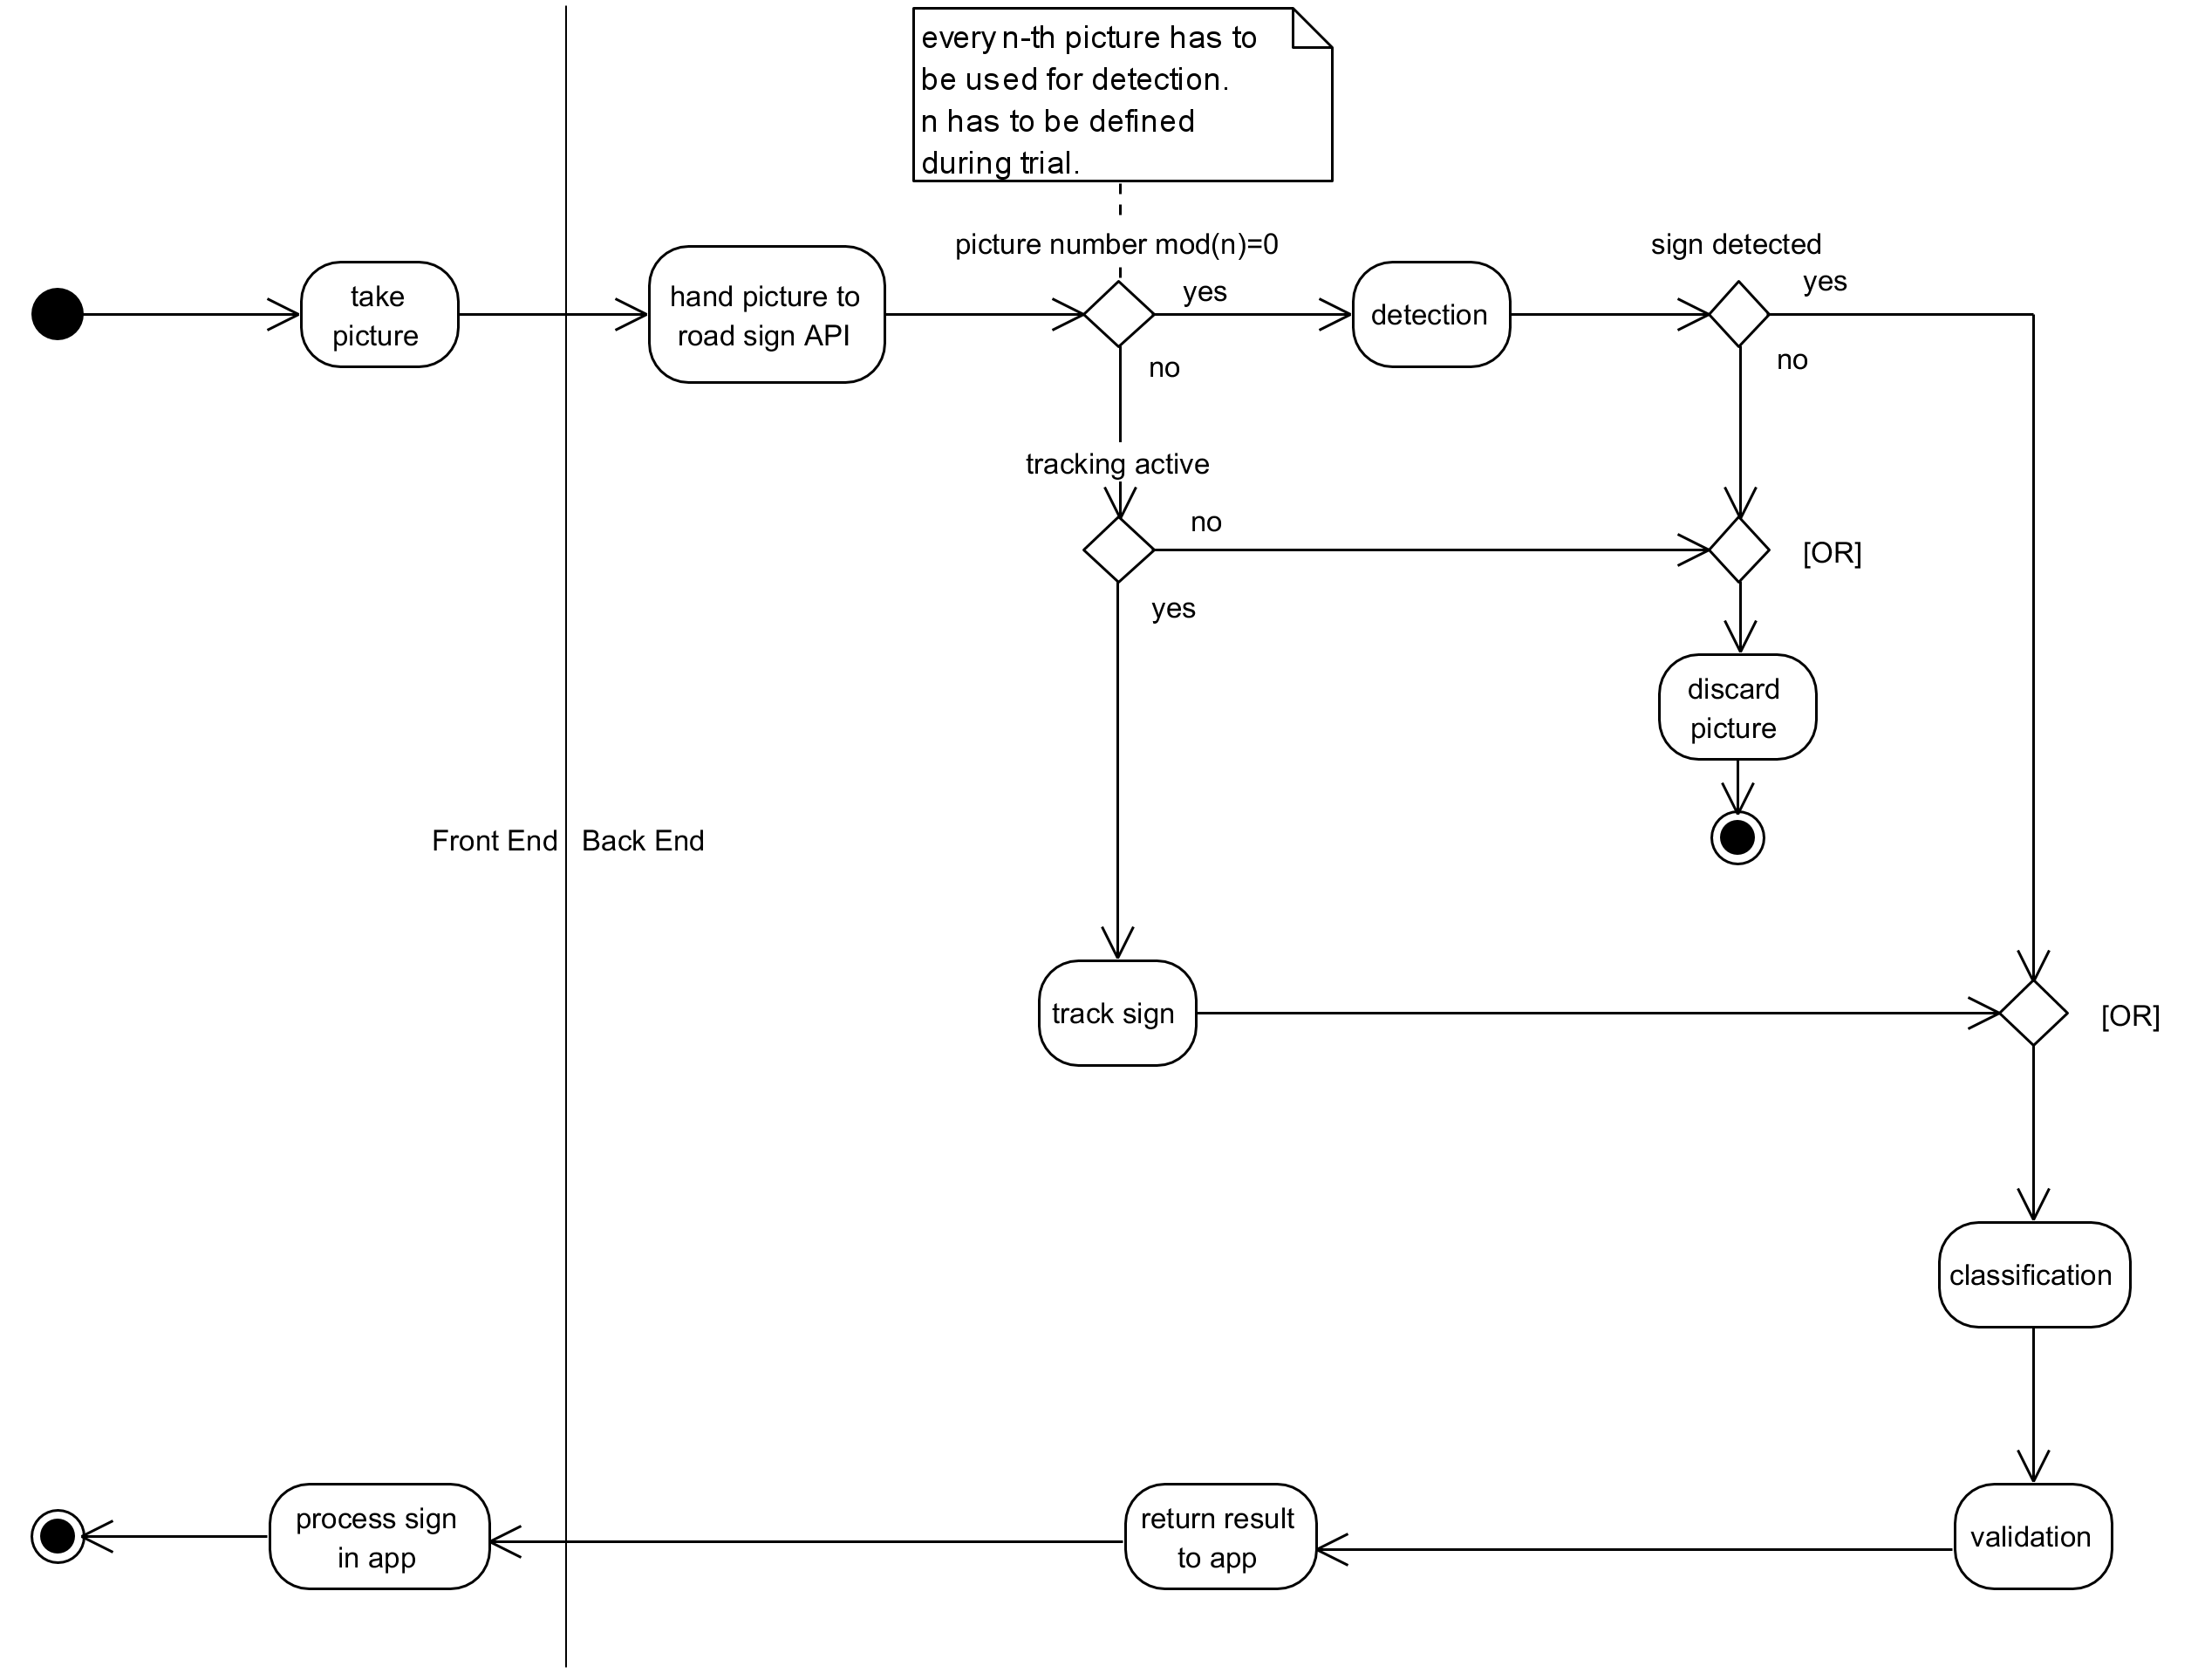
\includegraphics[width=1\linewidth]{Grafiken/Activity_Diagram.png}
\caption{Erkennung eines Verkehrszeichens aus Sicht der \gls{API}}
\end{figure}

Aus Abb. 5.3 ist ersichtlich, dass jedes n-te Bild zur \gls{Detektion} verwendet wird. Der Sinn und Zweck dabei ist, dass wir nicht jedes Bild der Kamera videotaktschritthaltend bearbeiten können. Wird also jedes n-te Bild zur \gls{Detektion} verwendet, werden alle anderen (1, 2, … , n-1) Bilder zum \gls{Tracking} verwendet.
Das \gls{Tracking} ist eine klassische Technik, nach der anhand von sehr einfachen Merkmalen im Bild die Position eines Objektes nachverfolgt (getrackt) werden kann. Dieses Verfahren funktioniert deutlich schneller als die \gls{Detektion}. Auf diese Art und Weise kann das Verkehrszeichen so lange getracked werden,  bis es sehr nah vor der Kamera ist und so ein besseres Bild zur Klassifizierung erlangen. Wurde allerdings bei der letzten \gls{Detektion} kein Verkehrszeichen gefunden, findet auch kein \gls{Tracking} statt und der Prozess wird abgebrochen.
Wie groß n zu sein hat, also wie viele Bilder getracked werden, bis das nächste mal Detektiert wird, muss in Versuchen unsererseits herausgefunden werden. Ist n zu klein, würde unnötig oft detektiert werden, was nicht nur zu viel Leistung beansprucht, sondern auch eine gewisse Fehlerwahrscheinlichkeit mit sich bringt. Ist n zu groß, würde ein Verkehrszeichen zu lange getracked werden und das darauf folgende Verkehrszeichen übersehen.
Die Validierung des klassifizierten Verkehrszeichens besteht daraus, dass mitgezählt wird, wie oft das gleiche Zeichen klassifiziert wurde. Wurde beispielsweise fünfmal \gls{VZ} 274-30 und einmal \gls{VZ} 274-80 klassifiziert, kann man sinnvollerweise davon ausgehen, dass es sich tatsächlich um \gls{VZ} 274-30 handelt und \gls{VZ} 274-80 eine Fehlklassifikation war. Die Fehlklassifikation wird in dem Fall auch nicht an die \gls{App} weitergegeben.

Abb. 5.2 und 5.3 beschreiben den globalen Kontrollfluss ausreichend. Da die \gls{App} und die \gls{API} möglichst unabhängig voneinander funktionieren, ergibt es relativ wenig Sinn, den Kontrollfluss von beiden im selben Diagramm zu zeichnen.\\


\subsection{Architekturmuster}

Die  \gls{Filterverwaltungs-Bibliothek}  ist nach dem \glslink{Pipes and Filters}{Pipes-and-Filters}-Prinzip aufgebaut. Dieses ist ein gängiges Architekturmuster für \glslink{System}{Systeme}, die Datenströme verarbeiten. In unserem Fall bestehen diese aus (einer Folge von) Einzelbildern mit einem Header, in dem Zusatzinformationen Platz finden. 
Ein \gls{Filter} stellt dabei einen Verarbeitungsschritt dar, wobei jeder \gls{Filter} der \gls{Pipe} ein Bild entgegennimmt und auch wieder ein Bild herausgibt. Darüber hinaus kann jeder \gls{Filter} dem Datenpaket bestimmte Metainformationen beifügen, die später für eine genauere Analyse verwendet werden können. Wenn beispielsweise ein \gls{Filter} ein Verkehrszeichen auf einem Bild an einer bestimmten Position detektiert und im darauffolgenden \gls{Filter} das Verkehrszeichen klassifiziert wird, wird neben dem Zuschneiden des Bildes auf das erkannte Verkehrszeichen auch die Position des Verkehrszeichens im Original als Metainformation gespeichert. Dies ist eine Abwandlung der herkömmlichen \glslink{Pipes and Filters}{Pipes-and-Filters}-Architektur.
Weiterhin ist es möglich, dass sich die \glslink{Pipe}{Pipeline} nach bestimmten Verarbeitungsschritten in mehrere untergeordnete \glslink{Pipe}{Pipes} aufteilt: Werden auf einem Bild mehrere Verkehrszeichen erkannt, wird der \gls{Filter} für die \gls{Klassifikation}  für alle Kandidaten aufgerufen (ggf. parallel). Dies erweitert die originale Architektur zum “Tee-and-Joins-\glslink{Pipes and Filters}{Pipes-and-Filters}-Pipeline-System”.
Die Wahl dieses Architekturmusters begründen wir wie folgt:

\subsubsection{Effizienz}
Alle \gls{Filter} einer \gls{Pipe} arbeiten auf ein- und demselben Datenobjekt im Speicher. Das heißt, dass jeder \gls{Filter} dieses Objekt per Adresse direkt anspricht, ohne es zu  kopieren. 

\subsubsection{Modularität}
Einzelne \gls{Filter} lassen sich individuell austauschen, erweitern oder entfernen. So lassen sich in unserem Fall z.B. einfach \gls{Filter} für verschiedene \glslink{Detektion}{Detektionsstrategien} oder optische Bildaufbereitung einfügen.

\subsubsection{Performanz}
Die Verwendung des \glqq{}Tee-and-Joins-\glslink{Pipes and Filters}{Pipes-and-Filters}-\glslink{Pipe}{Pipeline}-Systems\grqq{} erlaubt es 
uns, verschiedene Filteroperationen durch Verwendung mehrerer Threads 
echt-parallel zu bearbeiten und so Rechenzeit einzusparen.\\

\subsection{Wiederverwendbarkeit}
Aufgrund der Modularität nach 1. lässt sich die \glslink{Pipe}{Pipeline} Architektur für verschiedenste Aufgaben, über \glslink{Detektion}{Detektions-} und \glslink{Klassifikation}{Klassifikationsprobleme} hinaus, konfigurieren. Hierfür müssen lediglich die gewünschten \gls{Filter} implementiert werden, welche über genau spezifizierte Schnittstellen die Daten von der \gls{Pipe} bekommen und sie wieder an diese abgeben können.


\chapter{Entwurfsalternativen}

Die Wahl für zwei \gls{API}s statt nur einer ist darin begründet, dass die komplette Verkehrszeichenerkennung aus der \gls{App} auslagert werden soll (die \gls{App} stellt lediglich das Front-End dar), gleichzeitig die \gls{API} aber verschiedene \glslink{Detektion}{Detektions}- und \glslink{Klassifikation}{Klassifikationsprobleme} lösen kann, nicht nur die Verkehrszeichenerkennung. Deshalb wird die  \gls{Filterverwaltungs-Bibliothek}  möglichst allgemeingültig gehalten und soll nach einer entsprechenden Konfiguration für verschiedene Problemstellungen funktionieren. Die \gls{Verkehrszeichen-API} ist im Gegensatz dazu konkret auf das Problem der Verkehrszeichenerkennung spezialisiert und soll auch nur diesen Zweck erfüllen. Obwohl die Entscheidung für zwei \gls{API}s zunächst unnötig komplex erscheinen mag, sehen wir es als deutlich sinnvolleres und einfacheres Modell an.
Die andere Möglichkeit wäre es, keine \gls{Verkehrszeichen-API} zu erstellen und sämtliche Zwischenergebnisse direkt in der \gls{App} zu loggen und auch die Konfiguration der \gls{Filterverwaltungs-Bibliothek} in der \gls{App} umzusetzen. Diese Herangehensweise würde nicht nur die Portabilität deutlich einschränken, es würde auch zu einer unnötig hohen Kopplung der \gls{App} mit der \gls{API} kommen, was im Sinne der Softwaretechnik nicht erwünscht ist. Ferner ließe sich nicht mehr garantieren, dass die Verkehrszeichenerkennung auf allen Endgeräten gleich, oder zumindest ähnlich gut funktionieren wird, da wir auf Konfiguration der  \gls{Filterverwaltungs-Bibliothek}  zur Verkehrszeichenerkennung auf anderen Endgeräten keinen Einfluss mehr hätten.
Dadurch, dass die \gls{Verkehrszeichen-API} die  \gls{Filterverwaltungs-Bibliothek}  konfiguriert und aus Sicht der \gls{App} weitestmöglich abstrahiert, kann auch auf anderen Geräten von korrektem Verhalten zur Verkehrszeichenerkennung ausgegangen werden.\\

%%%%%%%%%%%%%%%%%%%%%%%%%%%%%%%%%%%%%%%%%%%%%%%%%%%
%%%%%%%%%%%%%%%%%% P H A S E - 2 %%%%%%%%%%%%%%%%%%
%%%%%%%%%%%%%%%%%%%%%%%%%%%%%%%%%%%%%%%%%%%%%%%%%%%
\part{Feinentwurf}\label{part:feinentwurf}

\chapter{Allgemeines}
Im Folgenden sei nach dem Grobentwurf auch der Feinentwurf der einzelnen Subsysteme erläutert. Während sich der Grobentwurf auf das System im Ganzen sowie auf die Kommunikation der Subsysteme untereinander bezog, werdem im Feinentwurf die einzelnen Subsysteme modelliert. Das Zusammenspiel der Subsysteme ist hier nicht von Relevanz und wird falls nötig maximal stark abstrahiert dargestellt.\\
Da das Agile Vorgehensmodell gewählt wurde und unnötiger Entwurfs-Overhead dementsprechend möglichst vermieden werden soll, wird dieser Teil lediglich die wichtigsten Details des Feinentwurfes beschreiben. Details, welche \glqq{}on the fly\grqq{} in der Implementierung entschieden wurden, werden hier nicht erwähnt, um unnötige Redundanzen zwischen dem Feinentwurf und der Entwicklerdokumentation zu vermeiden.\\

Der Feinentwurf ist nicht als Entwicklerdokumentation zu verstehen, da sich das implementierte System vom Feinentwurf unterscheiden kann. Die wirklich verbindlichen Klassendiagramme und Erklärungen befinden sich nicht hier, sondern in der Entwicklerdokumentation.\\


\chapter{Schnittstellendokumentation}


\section{App zu API}
\label{sec:schnittstellendokuAPPAPI}

\subsection{Übersicht}

Die Kommunikation zwischen der in Java geschriebenen App und der in C++ programmierten API wird über das Java Native Interface (JNI) realisiert. Dieses ermöglicht das Aufrufen gesondert gekennzeichneter C++ Funktionen von Java aus. Der in der App benötigte Funktionsumfang wird über zwei solcher Funktionen gewährleistet.\\

\subsection{Initialisierung}

Bevor die API zur Verkehrszeichenerkennung verwendet werden kann, muss diese einmalig initialisiert werden. Dafür ist eine JNI Funktion \texttt{initRoadSignAPI()} implementiert, welche nach dem Start der App aufgerufen wird und mit der zusätzlichen Information über die Anzahl der von TensorFlow zu verwendenten Threads die API initialisiert.\\

\subsection{Verkehrszeichenerkennung}

Für die Erkennung von Verkehrzeichen auf einem Bild muss dieses im RGB-Format an die Pipeline der API übergeben werden. Das RGB-Format sieht dabei pro Pixel die Farbkanäle Rot, Grün und Blau vor.
Die von der App angefragten Kamerabilder befinden sich allerdings im YUV-Format, welches jeden Pixel in die Komponenten Luminanz (Kanal Y) und Chrominanz (Kanäle U und V) aufteilt. Zusätzlich dazu kann die Schrittweite der Pixel im U Kanal je nach Gerät verschieden sein.
Es ist also eine Konvertierung des Kamerabilders in RGB unter Beachtung der Schrittweite von Nöten, bevor es verwendet werden kann.\\
Dazu wird zunächst der komplette Y Kanal in einen Byte-Array geschrieben, welcher den Platz für alle drei Kanäle besitzt. Dann wird die Schrittweite des U Kanals ermittelt.\\
Sollte diese eins betragen, so kann ebenfalls zunächst der U und dann der V Kanal auf die selbe Weise in den Byte-Array geschrieben werden. Diese Anordnung der YUV Bytes wird mit I420 bezeichnet.\\
Beträgt die Schrittweite jedoch zwei, so wird zunächst auch der U Kanal in den Array übertragen. Allerdings befindet sich in diesem Teil des Arrays nun nach jedem Pixel genau ein Byte Platz. Dieser Platz wird nun mit den dazugehörigen Daten im V Kanal aufgefüllt. Diese Anordnung wird mit NV21 bezeichnet.\\
Der ermittelte YUV-Array wird nun zusammen mit den Informationen über die Dimensionen des Bildes, über die Schrittweite und mit einem vorbereiteten Integer-Array für zurückzugebende ARGB-Daten an eine JNI Funktion \texttt{roadSignAPIfeedImage()} für die Verkehrszeichenerkennung übergeben.\\
Dort werden die YUV-Daten mithilfe von OpenCV unter Beachtung des YUV-Formats in RGB-Daten umgerechnet und von der Pipeline auf Verkehrszeichen untersucht.\\
Für die Rückgabe und Verwendung des umgerechneten Bildes in Java wird dieses in den übergebenen Integer-Array in ARGB-Form (mit Transparenz-Kanal A) geschrieben.\\
Die erkannten Verkehrszeichen werden als Verkehrszeichenkombinationen in Form des Rückgabewertes an Java weitergegeben. Dies ist in einem zweidimensionalen Integer-Array realisiert, in welchem je ein Integer-Array eine Verkehrszeichenkombination darstellt. Der erste Wert in einem solchen Array beinhaltet dabei die Anzahl der Verkehrszeichen in der Kombination. Für jedes dieser Verkehrszeichen folgt darauf jeweils die erkannte Klassen-Id des Zeichens, der x- und y-Wert der oberen linken Ecke im Bild und der x- und y-Wert der unteren rechten Ecke im Bild. Somit werden pro Verkehrszeichen 5 Arrayfelder benötigt.\\
Mit den ARGB-Daten des Bildes können die Informationen über die erkannten Verkehrszeichenkombinationen unter Java nun in den eigenen Datentyp für Verkehrszeichenkombinationen umgewandelt werden. Diese lassen sich dann für den weiteren Verlauf des Zwischenspeicherns und Anzeigens auf dem Display verwenden.\\

\section{API zu Neuronale Netze}
\label{sec:schnittstellendokuAPINN}
Damit die API die Neuronalen Netzwerke verwenden kann, müssen diese zunächst einmal nach dem Training in einem entsprechenden Format abgespeichert werden, um dann innerhalb der entsprechenden Benutzerumgebung (z.B. der Android App) wieder geladen werden zu können. TensorFlow verwendet hierfür standardmäßig das \gls{Protobuf} (Protocol Buffers) Format. Protocol Buffers bezeichnet Google's programmiersprachen- und plattformunabhängiges Format für die Serialisierung und Deserialisierung strukturierter Daten. Hierfür muss neben der TensorFlow Bibliothek an sich auch die dazugehörige Protobuf Bibliothek (als Teil von TensorFlow) eingebunden werden.
Die für die Interaktion mit den Neuronalen Netzen benötigten Funktionen stellt die Filterverwaltungs-Bibliothek zur Verfügung, welche hierfür eigene Klassen für die Anbindung an Tensorflow implementiert.
Das generelle Vorgehen sei dabei wie folgt erläutert:


\begin{enumerate}
    \item Erstellen einer neuen TensorFlow Session für das Netzwerk: Eine TensorFlow Session bezeichnet einen bestimmten Arbeitsbereich innerhalb dessen Berechnungen und Operationen ausgeführt werden. Pro Netzwerk wird, zumindest in unserem Fall, eine eigene Session erstellt.
    \item Laden der Netzwerk Repräsentation aus der Protobuf Datei.
    \item Erstellen eines Tensorflow Graphen aus der Protobuf Datei. TensorFlow benutzt zur Ausführung der Neuronalen Netzwerke das Prinzip der Datenstromorientierten Programmierung anhand von Datenstrom Graphen (dataflow graph). Dies ist ein verbreitetes Programmierprinzip für parallele Datenverarbeitung. Jeder Knoten in diesem Graphen repräsentiert einzelne Berechnungsschritte, und alle Kanten symbolisieren Daten die von einem Knoten erzeugt oder verwendet werden.
    \item Freigeben der Protobuf Datei um Speicherplatz einzusparen: Da das Netzwerk nun als Graph Repräsentation vorliegt kann die Protobuf Datei wieder aus dem RAM freigegeben werden.
    \item  Innerhalb eines TensorFlow Netzwerkes (und dann auch im Graphen) haben die einzelnen Knoten (Nodes) bestimmte Namen. Praktisch jeder dieser Knoten lässt sich über diesen Namen direkt ansprechen. Für die Interaktion mit dem Netzwerk muss abschließend noch festgelegt werden, welcher Knoten als Eingabe, und welche als Ausgabe dienen (mehrere Ausgabeknoten sind möglich). Diese können dann über die entsprechenden TensorFlow Funktionen angesprochen und gegebenenfalls ausgewertet werden.
\end{enumerate}



\chapter{Geplanter Entwurf}
\section{Feinentwurf der \gls{App}}
Die einzelnen \gls{App}-Menüs werden durch Fragmente realisiert, welche allesamt von der Basisklasse \texttt{FragmentActivity} aus dem Android-Framework abgeleitet sind.\footnote{\link{https://developer.android.com/reference/android/support/v4/app/FragmentActivity}, 26.05.2018} Jedes Fragment besitzt ein \gls{UI}-Layout sowie Hauptfunktionalität, die es erfüllen soll, während sekundäre Funktionalitäten sinnvollerweise in eigene Klassen ausgelagert werden. So soll beispielsweise im Verkehrszeichenerkennungsfragment auch die aktuelle, mit GPS ermittelte Geschwindigkeit, angezeigt werden - in dem Fall wäre die Geschwindigkeitsermittelung eine eine Klasse (aber kein Fragment), die aus dem Detektorfragment aufgerufen wird.\\
In \cref{fig:klassen_app} auf der nächsten Seite befindet sich ein Klassendiagramm zur groben Übersicht und im Folgenden seien die einzelnen Klassen kurz erläutert.\\

\begin{landscape}
\begin{figure}
\label{fig:klassen_app}
\centering
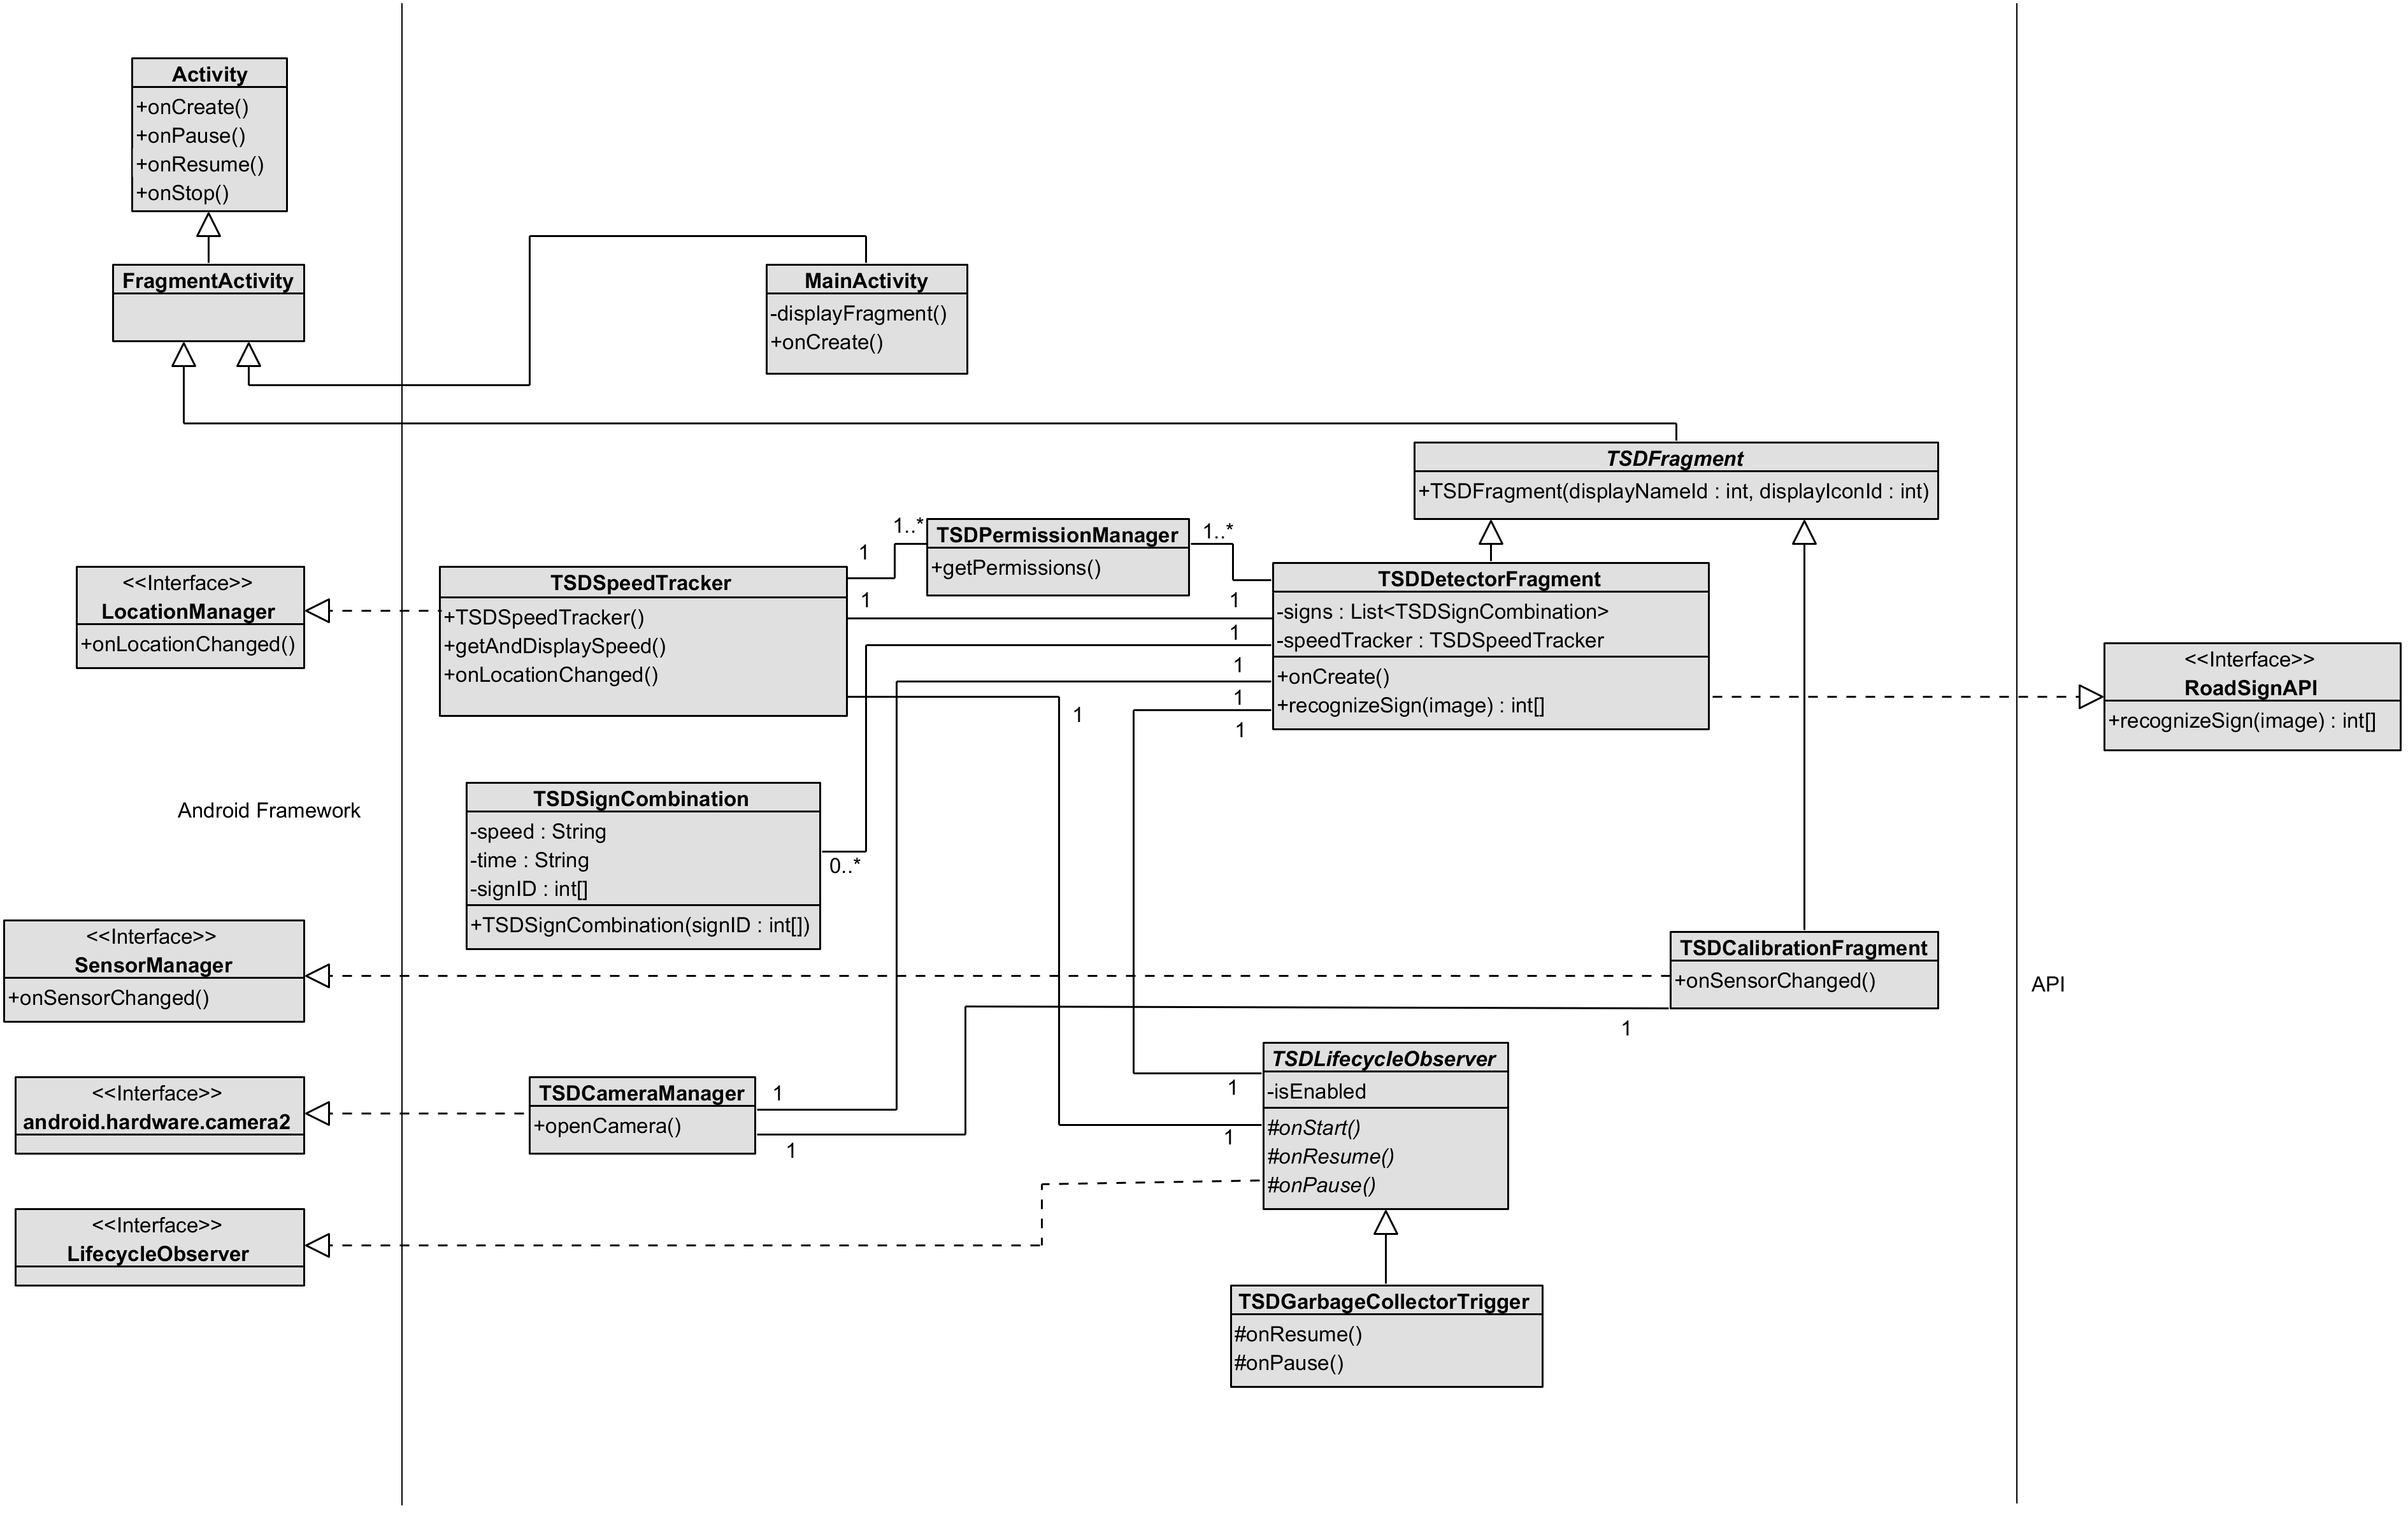
\includegraphics[width=0.95\linewidth]{Reviewdokument/Grafiken/app_class_diagram.png}
\caption{UML-Klassendiagramm der \gls{App}}
\end{figure}
\end{landscape}

\subsubsection*{MainActivity}
Die Klasse \texttt{MainActivity} ist die Aktivität, in der die Mensch-Maschine-Interaktion stattfindet. Der Zweck dieser Klasse ist es, einzelne Fragmente (sh. \texttt{TSDFragment}) zu laden, und so einen Wechsel zwischen verschiedenen Menüs zu ermöglichen. Sie wird von der Basisklasse \texttt{FragmentActivity} aus dem Android-Framework abgeleitet.\\

\subsubsection*{TSDFragment}
\texttt{TSDFragment} ist eine abstrakte Klasse, aus der die einzelnen Fragmente, welche ein \gls{UI} besitzen abgeleitet werden können. Es können selbstverständlich keine Objekte vom Typ \texttt{TSDFragment} als solchem angelegt werden, nur von dessen abgeleiteten Klassen. In der \texttt{MainActivity} werden veschiedene, von \texttt{TSDFragment} abgeleitete Klassen mit \gls{UI} und entsprechender Funktionalität geladen.\\

\subsubsection*{TSDDetectorFragment}
Diese Klasse ist aus \texttt{TSDFragment} abgeleitet und stellt die Hauptfunktionalität der App, nämlich die Verkehrszeichenerkennung, dar. Hier soll die Kommunkation zwischen der App und der \gls{Verkehrszeichen-API} erfolgen; es sollen die mit der Kamera aufgenommenen Bilder an die \gls{Verkehrszeichen-API} übergeben werden und neue Objekte vom Typ \texttt{TSDSignCombination} (sh. u.) angelegt werden.\\

\subsubsection*{TSDCalibrationFragment}
Die Klasse \texttt{TSDCalibrationFragment} stellt die Kalibrierung dar. Mittels des Rotationsvektorsensors des Gerätes, welcher mit \texttt{SensorManager} aus dem Android-Framework abgefragt werden kann, soll entschieden werden, ob das Gerät gerade hängt oder noch vom Nutzer angepasst werden soll.\\

\subsubsection*{TSDSpeedTracker}
Soll aus \texttt{TSDDetectorFragment} aus aufgerufen werden und jenes Fragment mit der Information über die aktuelle, mittels GPS gemessene, Geschwindigkeit versorgen. Da die Geschwindigkeitsanzeige sinnvollerweise Teil des Detektorfragmentes und kein einzelnes Menü sein soll, ist \texttt{TSDSpeedTracker} nicht von der Basisklasse \texttt{TSDFragment} abgeleitet.\\

\subsubsection*{TSDSignCombination}
Mittels dieser Klasse werden in der \gls{App} die erkannten Verkehrszeichen als Objekt angelegt. Neben einem Array aus \texttt{signID}s, in welchem die \gls{VZ}-Nummern der erkannten Verkehrszeichen enthalten sind, gehört zu jedem Objekt des Typs \texttt{TSDSignCombination} auch der Zeitpunkt der Erkennung sowie die dabei gemessene Geschwindigkeit.\\
Die Idee dabei ist, dass von der \gls{Verkehrszeichen-API} (\texttt{RoadSignAPI}) beispielsweise das Array \texttt{[131, 27470]} zurückgegeben wird und in der App entsprechend ein neues Objekt vom Typ \texttt{TSDSignCombination} mit eben diesen Werten angelegt wird. Bei der weiteren Verarbeitung werden die Grafiken für \gls{VZ} 131 (Lichtzeichenanlage) und \gls{VZ} 274-70 (zul. Höchstgeschw. 70 km/h) gesucht und dem Nutzer angezeigt.\\

\subsubsection*{TSDCameraManager}
Der von Android bereitgestellte Zugriff auf die Smartphonekamera ist zwar umfangreich aber auch relativ komplex. Deshalb soll es die Klasse \texttt{TSDCameraManager} geben, um diese Schnittstelle aus Sicht der App zu abstrahieren und zu weitestmöglich vereinfachen.\\

\subsubsection*{TSDPermissionManager}
Eine \gls{App} benötigt unter Android zur Laufzeit gewisse Berechtigungen, deren Anfrage der \gls{Nutzer} ggf. auch zurückweisen kann. Um z.B. auf die Kamera oder auf die Standortermittelung zugreifen zu können, muss die \gls{App} den Nutzer um die entsprechende Berechtigung bitten, und der Nutzer muss diese Berechtigung erteilen, ansonsten wird eine \texttt{exception} geworfen. \texttt{TSDPermissionManager} soll dazu dienen, die \gls{App}-Berechtigungen einfacher zu verwalten. \\

\subsubsection*{TSDLifecycleObserver}
Diese Klasse soll vermeiden, dass die \gls{App} weiterhin im Hintergrund berechnungen anstellt, während sie z.B. pausiert ist. Dazu gibt es im Android-Framework eine ganze Reihe an Methoden, die bei den entsprechenden Ereignissen automatisch aufgerufen werden, z.B. \texttt{onStart}, \texttt{onPause} und \texttt{onResume}.\\

\subsubsection*{TSDGarbageCollectorTrigger}
Während der Implementierung fiel auf, dass unter Android 8 \glqq{}Oreo\grqq{} ein Memory Leak bei der Kamera existiert. Um dieses Memory Leak vorzubeugen, existiert die Klasse \texttt{TSDGarbageCollectorTrigger}, welche in bestimmten Zeitabständen periodisch den Java-Garbage-Collector aufruft.\\

\subsubsection*{RoadSignAPI}
Java-Schnittstelle der \gls{Verkehrszeichen-API}. Ist im nächsten Kapitel genauer erläutert.\\

\subsubsection*{Android-Framework}
Alle Klassen im linken Drittel des Diagrammes gehören zu dem Android-Framework und wurden nicht in diesem Projekt entworfen, dementsprechend seien sie hier nicht genauer erläutert. Erklärungen zu jeder dieser sechs Klassen befinden sich in der umfangreichen Android-Entwicklerdokumentation\footnote{\link{https://developer.android.com/reference/packages}, 12.06.2018}.\\

\section{Feinentwurf der APIs}
Wie bereits im Grobentwurf (sh. \cref{sec:subsystemstruktur}) beschrieben, besteht die \gls{API} aus zwei Komponenten - der \gls{Filterverwaltungs-Bibliothek} und der \gls{Verkehrszeichen-API}, wobei die \gls{Verkehrszeichen-API} die \gls{Filterverwaltungs-Bibliothek} benutzt, um verschiedene Filter zu implementieren, welche z.B. den Input zuschneiden oder \glslink{Neuronales Netzwerk}{Neuronale Netze} auf den Input anwendet. Die \gls{Filterverwaltungs-Bibliothek} ist nach dem Pipes-and-Filter-Prinzip aufgebaut, auch dies wurde im Grobentwurf hinreichend erläutert und wird verfeinert in dem zugehörigen Klassendiagramm aus \cref{fig:klassen_api} dargestellt.\\

\begin{landscape}
\begin{figure}
\label{fig:klassen_api}
\centering
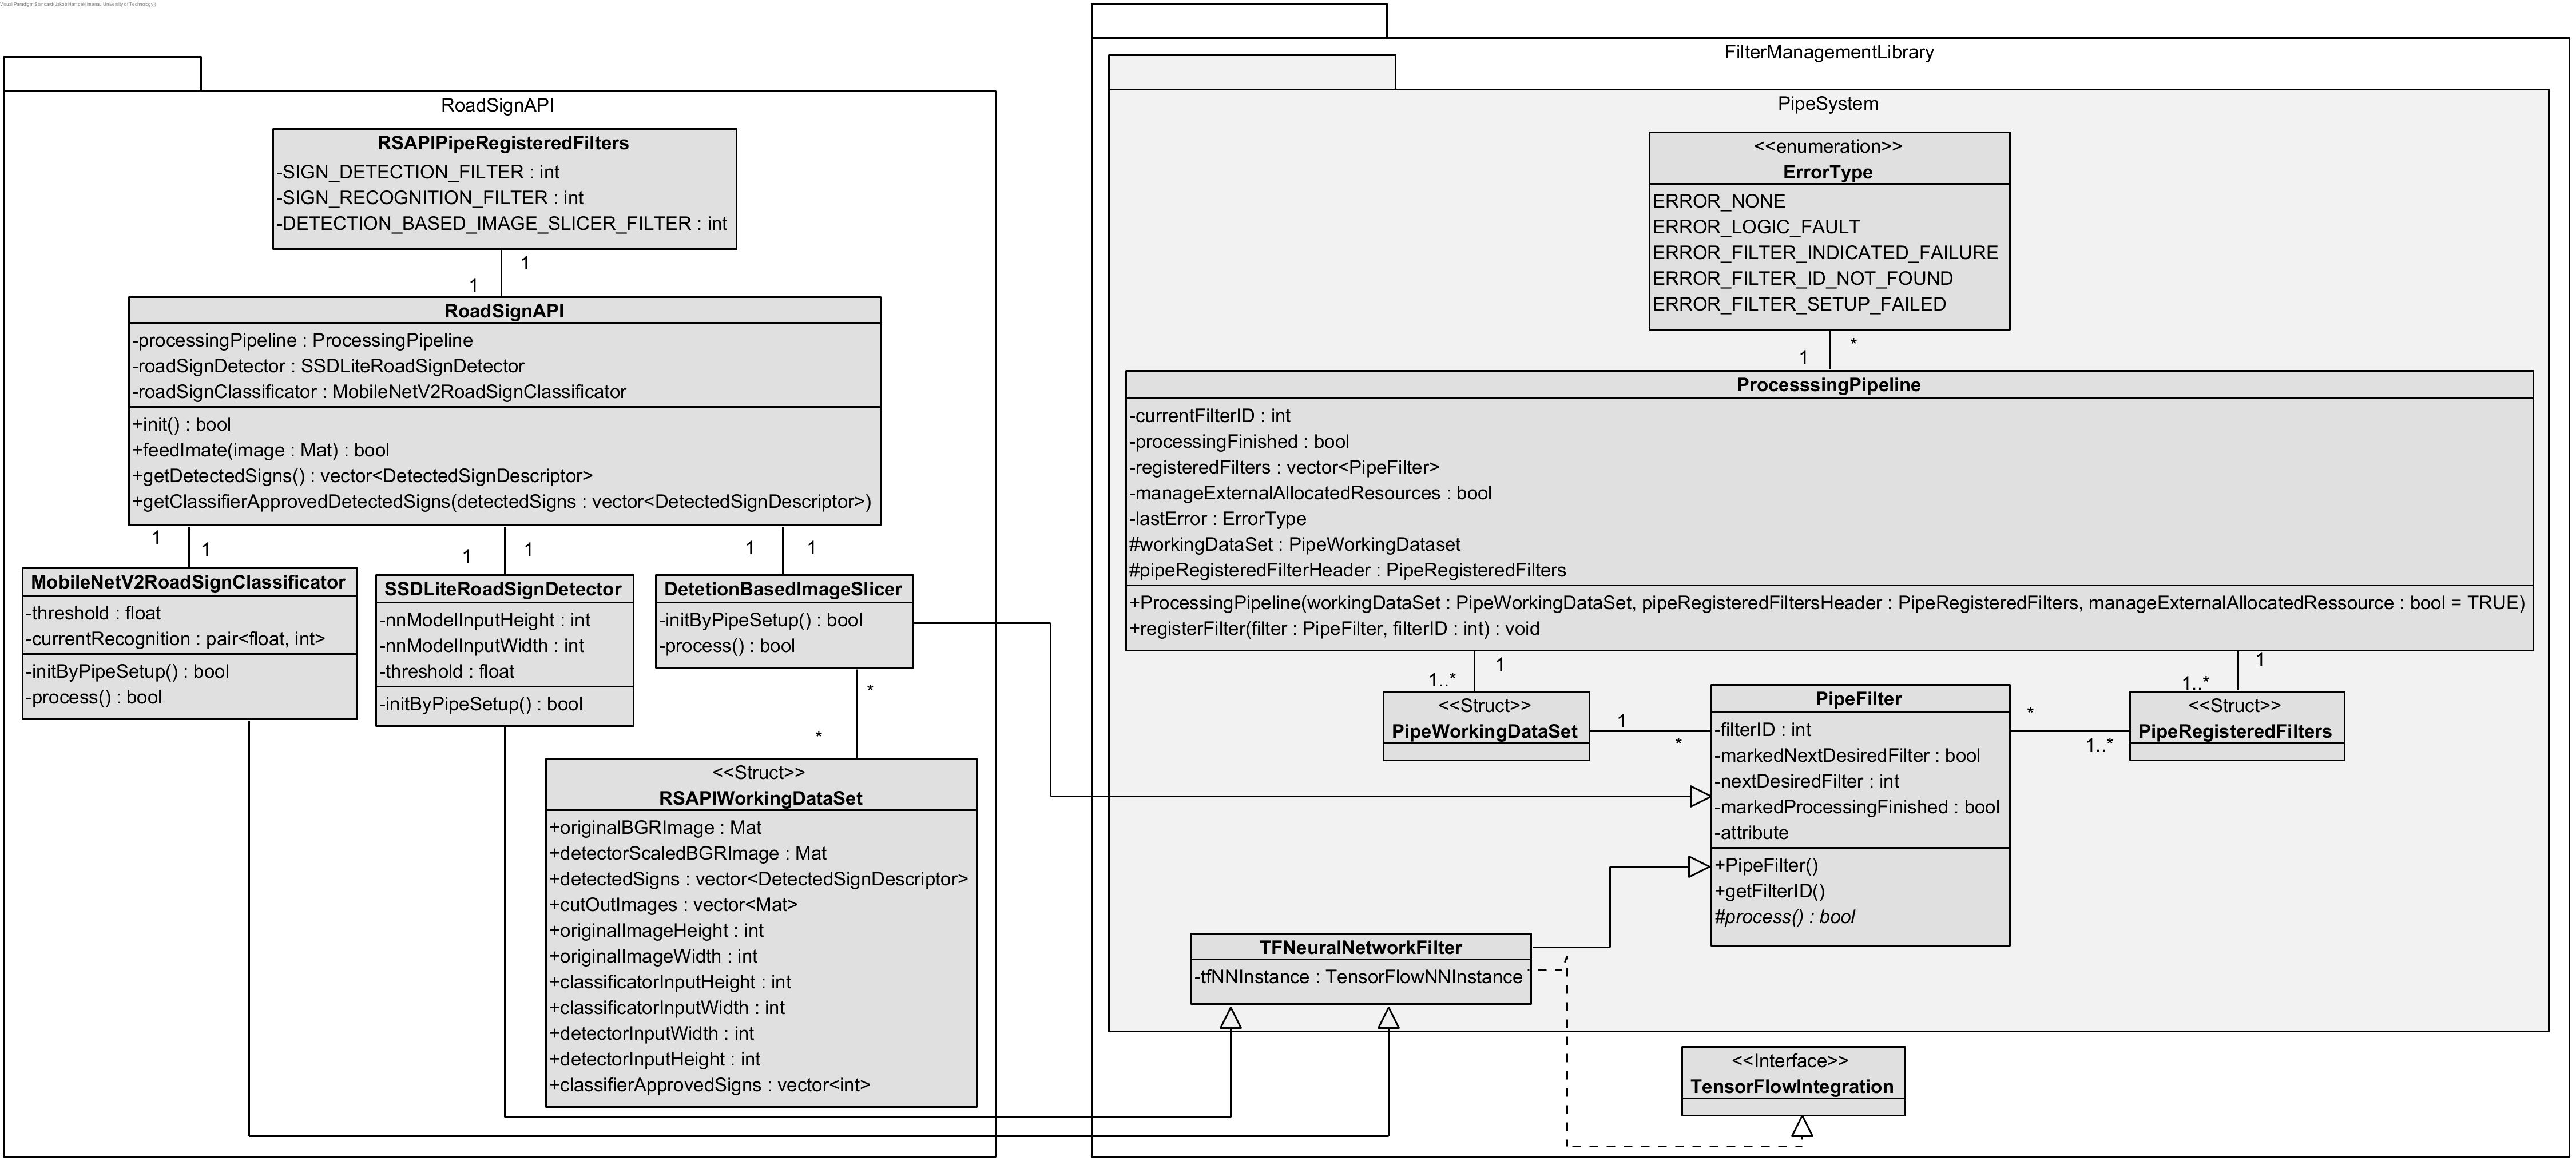
\includegraphics[width=1.08\linewidth]{Reviewdokument/Grafiken/api_class_diagram.png}
\caption{UML-Klassendiagramm der \gls{API}}
\end{figure}
\end{landscape}

\subsection{Filterverwaltungs-Bibliothek und Verkehrszeichen-API}
Im folgenden sei der Begriff \gls{Verkehrszeichen-API} gleichwertig mit RoadSignAPI und der Begriff \gls{Filterverwaltungs-Bibliothek} gleichwertig mit FilterManagementLibrary. Die englischen Bezeichnungen wurden gewählt, weil dies gängige Programmierpraktik ist und auch in der Entwicklerdokumentation so referenziert werden.\\


\subsection{Filterverwaltungs-Bibliothek}
Die Filterverwaltungs-Bibliothek wurde der entsprechend der Spezifikation aus der ersten Phase umgesetzt (siehe Reviewdokument Phase 1, Kapitel 6, insbesondere Unterpunkt 6.1.2).
Die einzelnen Komponenten seien im Folgenden erläutert.\\
\subsubsection*{ProcessingPipeline}
Die \texttt{ProcessingPipeline} stellt  die Pipe der Pipes-and-Filters-Architektur dar. Sie steht im Mittelpunkt der \gls{Filterverwaltungs-Bibliothek}. Hier werden die Filter registriert, verwaltet und ausgeführt. 
Die einzelnen Filter können der Pipeline hierbei Hinweise geben, was diese als nächstes tun sollte:
Jeder Filter muss, nachdem er aufgerufen wurde und seine Operationen ausgeführt hat, entweder anzeigen, welcher Filter als nächstes aufgerufen werden sollte, oder festlegen, dass die Verarbeitung der aktuellen Daten abgeschlossen ist. Letzteres hat zur Folge, dass kein weiterer Filter aufgerufen wird. Dies hat den Vorteil, dass, falls beispielsweise ein Detektor-Filter für ein Bild keine Detektionen ermitteln konnte, bereits an dieser Stelle die Bearbeitung abbrechen kann, ohne dass ein Klassifikator-Filter aufgerufen werden würde.
Jedem Filter wird außerdem von der Filterverwaltungs-Bibliothek eine eindeutige ID zugewiesen, die aus einer fortlaufenden Nummerierung generiert wird und stets größer als Null ist. 
Gegebenenfalls auftretende Fehler in unterschiedlichen Bereichen der Bibliothek, beispielsweise beim Initialisieren oder beim Aufrufen der Filter, werden entsprechend kommuniziert. Neben automatisch erzeugten Fehlermeldungen auf der Konsole können aufgetretene Fehler vom Anwender gesondert abgefragt und behandelt werden.\\

\subsubsection*{PipeFilter}
Die entsprechend zugehörigen Filter. Jeder Filter der \gls{Verkehrszeichen-API} ist direkt oder indirekt von dieser Klasse abgeleitet. Will man die \gls{Filterverwaltungs-Bibliothek} verwenden, muss man die verwendeten Filter ebenfalls von \texttt{PipeFilter} ableiten. Die Klasse wird zwar in diesem Projekt nur für die drei zuvor genannten Filter benutzt, kann aber in späteren Verwendungen beliebige Funktionen erfüllen - das Design dieser Klasse soll dahingehend keine Einschränkungen vorschreiben.\\

\subsubsection*{TFNeuralNetworkFilter}
Eine Subklasse von \texttt{PipeFilter}, die insbesondere zur Verwendung von Neuronalen Filtern vorbereitet ist. Sie unterscheidet sich von ihrer Elternklasse dadurch, dass sie die TensorflowIntegration Komponente der Filterverwaltungs-bibliothek benutzt um ein zur Anwendung bereites \gls{Neuronales Netzwerk} bereitzustellen. Entsprechend werden von \texttt{TFNeuralNetworkFilter} in der \gls{Verkehrszeichen-API} die Filter Klassifikations- und Detektionsfilter abgeleitet.\\\\

\subsubsection*{PipeRegisteredFilters}
Ein abstraktes Struct. Wie bereits erwähnt soll jeder in der Lage sein einen nachfolgenden Filter zu bestimmen. Hierfür muss die ID des Nachfolgers allerdings bekannt sein. Dieses Struct bietet Anwendern die Möglichkeit, durch entsprechendes Ableiten eine Liste der ID's und zugehörigen, eindeutigen Namen an alle Filter einer Pipeline zu verteilen.\\

\subsubsection*{PipeWorkingDataSet}
Die Daten bzw. der Datensatz auf dem die Pipeline arbeitet. Dies ist eine abstrakte Klasse. Für konkrete Realisierungen muss eine Klasse von dieser abgeleitet und den Bedürfnissen entsprechend mit Daten gefüllt werden. Der Datensatz einer Pipe wird mit allen Filtern geteilt, sodass ein direkter Zugriff ohne Kopieroperationen möglich ist.\\

\subsubsection*{ErrorType}
Ein einfacher Enumerator, welcher die ggf. auftretenden Fehlermeldungen beschreibt.
\begin{description}
\item \texttt{ERROR\_NONE} \\ Es trat kein Fehler auf.
\item \texttt{ERROR\_LOGIC\_FAULT} \\ Die Funktion \texttt{process()} eines Filters gab den Wert \texttt{true} zurück, der Filter hat aber weder einen nächsten Filter bestimmt, noch festgelegt dass die Bearbeitung der aktuellen Daten abgeschlossen ist.
\item \texttt{ERROR\_FILTER\_INDICATED\_FAILURE} \\ Die Funktion \texttt{process()} gab den Wert \texttt{false} zurück.
\item \texttt{ERROR\_FILTER\_ID\_NOT\_FOUND} \\ Die angegebene Filter-ID gehörte zu keinem bekannten Filter.
\item \texttt{ERROR\_FILTER\_SETUP\_FAILED} \\ Der Filter konnte nicht eingerichtet werden.\\
\end{description}

\paragraph{Anmerkung:} Der Bereich TensorflowIntegration wurde im Klassendiagramm im Gegenzug für bessere Übersichtlichkeit abstrakt dargestellt (der genaue Aufbau ist zumindest für die Nachvollziehbarkeit im Klassendiagramm zunächst nicht notwendig). Er stellt eine notwendige Abstraktion für die Anbindung an Tensorflow Mobile dar. Dafür wurden unter anderem Klassen zur strukturellen Beschreibung der Neuronalen Netze (Inputgröße und so weiter) sowie den generellen Umgang mit diesen (laden, auswerten et cetera.) implementiert.


\subsection{RoadSignAPI}
Die \gls{Verkehrszeichen-API} verwendet die Filterverwaltungs-Bibliothek für die Implementierung der Funktionalität der Verkehrszeichenerkennung. Sie kann prinzipiell als gewöhnliche Klasse betrachtet werden, welche sich beliebig oft instanziieren lässt (wenn gewünscht, auch mit unterschiedlichen Netzwerken pro Instanz).
Um die Anbindung an die \gls{App} zu ermöglichen, implementiert sie darüber hinaus zusätzlich ein statisches Interface, welches dafür eine spezielle Instanz der RoadSignAPI verwendet.
Bereitgestellt werden unter anderem die Funktionen \texttt{init()}, \texttt{feedImage(...)} und \texttt{getDetectedSigns()} zu finden, welche von der \gls{App} aufgerufen werden. Zu Beginn muss die Verkehrszeichen-API mit \texttt{init()} initialisiert werden. Mit \texttt{feedImage(...)} kann der \gls{Verkehrszeichen-API} ein Bild übergeben werden, welches unmittelbar bearbeitet wird: Werden auf dem Bild Verkehrszeichen erkannt, lassen sich diese über \texttt{getDetectedSigns()} zurückgeben.  Die \texttt{RoadSignAPI} besitzt eine Pipe und drei Filter - einen Detektor, einen Klassifkator sowie einen Filter zum Zuschneiden.\\

\subsubsection*{RSAPIPipeRegisteredFilters} Enthält die Attribute \texttt{SIGN\_DETECTION\_FILTER}, \texttt{SIGN\_CLASSIFICATION\_FILTER} und\\\texttt{DETECTION\_BASED\_IMAGE\_SLICER\_FILTER}, welche die IDs der drei eben benannten Filter sind. Gemäß der Beschreibung von PipeRegisteredFilters wird dieses Struct allen Filtern der Pipe übergeben, damit diese die IDs der jeweils anderen Filter kennen. \\

\subsubsection*{RSAPIWorkingDataSet}
Datensatz gemäß der Beschreibung von PipeWorkingDataSet. Hier werden diejenigen Daten gespeichert, die die RoadSignAPI für die Bearbeitung benötigt: Als Beispiel genannt seien zum Beispiel das originale Bild welches mit feedImage(...) übergeben wurde, eine Liste mit Structs vom Typ \texttt{DetectedSignDescriptor}, welches die erkannten Schilder beinhalten et cetera.  Da die \gls{Detektion} auf einer Auflösung von 300$\times$300 Pixeln ausgeführt wird, die \gls{Klassifikation} aber eine möglichst große Auflösung bekommen soll, müssen die Koordinaten dazu entsprechend umgerechnet werden und dann die detektierte Box möglichst aus dem großen Originalbild ausgeschnitten werden. Die für diese Umrechnung notwendigen Informationen werden ebenfalls aus diesem Verbund herangezogen.\\

\subsubsection{DetectedSignDescriptor}
Struct welches ein auf einem Bild detektiertes und klassifiziertes Verkehrszeichen beschreibt:
\begin{description}
\item \texttt{Punkt(x,y): upperLeft} \\ Bezogen auf das Rechteck innerhalb dessen ein Schild erkannt wurde, die Koordinaten oben links.
\item \texttt{Punkt(x,y): lowerRight} \\ Bezogen auf das Rechteck innerhalb dessen ein Schild erkannt wurde, die Koordinaten unten rechts.\\
\item \texttt{int: detectorPredictedClassID} \\ Klasse des Schildes, welche der Detektor ausgibt.
\item \texttt{float: detectorConfidence} \\ Sicherheit des Detektors beim Detektieren des Schildes (Wert zwischen 0 und 1)
\item \texttt{int: classifierPredictedClassID} \\ Klasse des Schildes, welche der Klassifikator ausgibt\
\item \texttt{float: classifierConfidence} Sicherheit des Klassifikators beim Klassifizieren des Schildes (Wert zwischen 0 und 1)\\
\end{description}

\subsubsection*{SSDLiteRoadSignDetector}
\glslink{Detektion}{Detektionsfilter}. Benutzt einen TFNeuralNetworkFilter um das Detektions-Netzwerk einzubinden. Der Filter bearbeitet die entsprechenden Bereiche des Datensatzes (\text{RSAPIWorkingDataSet}: Es verwendet das originale Bild und skaliert es auf die entsprechende Input Größe, welches anschließend dem Netzwerk übergeben werden. Die Ausgaben des Netzwerkes werden nun so interpretiert und aufbereitet, dass sie sich als \text{DetectedSignDescriptor} zwischenspeichern lassen.\\

\subsubsection*{DetectionBasedImageSilcer}
Schneidet anhand der von \texttt{SSDLiteRoadSignDetector} generierten Daten alle erfolgreich detektierten Verkehrszeichen aus; das bedeutet dass er Anhand der Attribute upperLeft und lowerRight für jeden erstellten DetectedSignDescriptor von \texttt{RSAPIWorkingDataSet} die entsprechenden Bereiche aus dem Originalbild in ein kleineres Bild kopiert.\\

\subsubsection*{MobileNetV2RoadSignClassificator}
\glslink{Klassifikation}{Klassifikationsfilter}. Benutzt einen TFNeuralNetworkFilter um das Klassifizierungs-Netzwerk einzubinden. Der Filter skaliert die vom \texttt{DetectionBasedImageSlicer} ausgeschnittenen Bildbereiche auf die erwartete Input Größe des Klassifikatornetzwerkes und verwendet dieses anschließend, um die detektierten Schilder zu klassifizieren.\\


\section{Feinentwurf der Neuronalen Netze}
\subsection{Detektion}
Zur Detektion wird \glqq{}SSDLite\grqq{}\cite{DBLP:journals/corr/abs-1801-04381} verwendet. Hierbei wurden frei verfügbare vortrainierte Gewichte benutzt.\footlinktext{https://github.com/tensorflow/models/blob/master/research/object_detection/g3doc/detection_model_zoo.md}{13.06.2018}
Dies wurde aus dem Hintergrund getan, dass man durch so genanntes \glqq{}Transfer learning\grqq{} auf schon bereits gelernte Merkmale aufbauen kann und diese lediglich angepasst werden.
Dadurch erreicht man vergleichbare Ergebnisse, spart sich jedoch erheblich viel Rechenzeit.
\subsubsection{Eingabe}
Als Eingabe für das \glslink{Neuronales Netzwerk}{Neuronale Netzwerk} werden RGB-Bilder, d.h. 3 Kanäle, der Größe 300$\times$300 Pixel benötigt.\\
Die Werte müssen, wie für den RGB-Standart üblich, in dem Bereich von 0-255 angegeben werden.
Dies wird in dem Datentypen uint(unsigned Integer) getan.
Da bei dem Labeln für das Training 16:9 Bilder verwendet wurden, mussten diese entsprechend herunterskaliert werden und in der Höhe noch zusätzlich gestreckt, damit die Bilder einer Auflösung von $300\times300$ vorliegen.\\
Zum Anpassen des Datensatzes an diese Anforderung wurde die quelloffene Grafikbibliothek \gls{OpenCV2} verwendet.
Bei der Skalierung wurde bikubische Interpolation verwendet, da beim Testen verschiedener Verfahren, dieses, von den zur Verfügung stehenden Verfahren, die kleinsten Gradienten an den Pixelübergängen erzeugt ohne das Bild stark unfokusiert wirken zu lassen, wie es sich beim Lanczos-Filter gezeigt hat.\\

\subsubsection{Ausgabe}
Das Netzwerk gibt für jedes eingegebene RGB-Bild das Ergebnis auf den, im Folgenden beschriebenen, vier Ausgabeknoten (\gls{Tensorflow Node}) zurück. Diese Ausgabeknoten besitzen innerhalb des Tensorflow Graphen (der aus der Model Datei erstellt wird) ganz bestimmte Bezeichnungen und repräsentieren alle unterschiedliche (Zwischen-)Ergebnisse der Ausgabe des Netzwerkes. Sie seien im Folgenden kurz erläutert.\\

\subsubsubsection*{1. Ausgabeknoten: num\textunderscore detections}
Der Knoten mit der Bezeichnung \texttt{num\textunderscore detections} gibt als Ergebnis eine Zahl vom Datentypen \texttt{uint} (unsigned integer) zurück.
Diese Zahl gibt an, wieviele Detektionen das Netzwerk zu dem gegebenen Input gefunden hat. \\

\subsubsubsection*{2. Ausgabeknoten: detection\textunderscore class}
Der Knoten mit der Bezeichnung \texttt{detection\textunderscore class} gibt ein eindimensionales \texttt{uint8}-Array der Länge 100 zurück. Das heißt, dass das Netzwerk maximal 100 verschiedene Detektion in einem Bild finden kann. Aufgrund der Ausgabe des Knotens  num\textunderscore detections weiß man, welche Einträge aus dem Array relevant sind; ist  num\textunderscore detections beispielsweise 10, müssen nur die ersten 10 betrachtet werden.
Jedes Element aus diesem Array gibt darüber Auskunft, zu welcher Klasse das detektierte Element gehört.\\
Die erste Klasse sind verschiedene Verkehrszeichen, welche keinen Einfluss auf die Geschwindigkeit haben. Die zweite Klasse sind geschwindigkeitsregulierende Verkehrszeichen und die dritte und letzte Klasse sind Zusatzzeichen.\\


\subsubsubsection*{3. Ausgabeknoten: detection\textunderscore score}
Der Knoten \texttt{detection\textunderscore score} gibt ein eindimensionales \texttt{float}-Array der Länge 100 zurück. Jeder Wert in dem Array liegt zwischen 0 und 1 und gibt an, wie sicher sich das Netzwerk bei der \gls{Klassifikation} ist. Hierbei steht eine 1 für 100\% und eine 0 für 0\%.\\
Es lässt sich wieder mit der Ausgabe des Knotens \texttt{num\textunderscore detections} der relevante Teil des Arrays abgrenzen. Alle Einträge des Array mit einem Index größer als num\textunderscore detections sind dann 0. \\

\subsubsubsection*{4. Ausgabeknoten: detection\textunderscore boxes}
Der Knoten detection\textunderscore boxes gibt ein zweidimensionales \texttt{float}-Array zurück. Hierbei ist die Länge des Arrays 100 und die Breite 4. Alle Zahlenwerte sind prozentual zu verstehen. So liegt, analog zur dritten Schicht, jeder Wert zwischen 0 und 1. 
Das erste Element beschreibt die prozentuale Position des linken Y-Achsen-Wertes, das zweite Elemente die Postition des linken X-Achsen-Wertes, das dritte Element die Position des rechten Y-Achsen-Wertes und das vierte und somit letzte Element den rechten X-Achsen-Wert. Diese 4 Angaben ergeben somit ein Rechteck um das detektierte Element.\\
Wenn weniger Objekte als die Array-Länge detektiert wurden, wird der Rest mit 0 gefüllt. Entsprechend lässt sich auch hier wieder \texttt{num\textunderscore classes} nutzen, um den relevanten Teil abzugrenzen.\\

\subsection{Klassifikation}
Zur \gls{Klassifikation} wird MobileNetV2\cite{DBLP:journals/corr/abs-1801-04381} mit vortrainierten Gewichten verwendet. Dabei wird das Modell für $96\times96$ Bilder verwendet, da dieses am wenigsten Rechenzeit beansprucht.
\subsubsubsection{Eingabe}
Als Eingabe für das \glslink{Neuronales Netzwerk}{Neuronale Netzwerk} werden RGB-Bilder der Größe $96\times96$ Pixel benötigt. Die Werte müssen im Bereich von -1 bis 1 angegeben werden, weshalb sie erst umgerechnet werden müssen, da diese üblicherweise im Bereich 0-255 angegeben sind.
Da die selbst erstellten \glslink{Sample}{Samples}, sowie die Bilder des GTSRB Datensatzes in unterschiedlichsten Größen vorliegen werden diese vor dem training auf eine Größe von $96\times96$ skaliert.
Dafür wird die bikubische Interpolation der Bibiliothek \gls{OpenCV2} verwendet. 

\subsubsubsection{Ausgabe}
Das \glslink{Neuronales Netzwerk}{Netzwerk} gibt für jedes eingegebene Bild ein eindimensionales \texttt{float}-Array mit der Länge der Klassen zurück.
Dabei steht jeder Eintrag in dem Array für eine Klasse, d.h für ein Verkehrszeichen bzw. eine Gruppe von Verkehrszeichen. Jeder Wert in dem Array liegt zwischen 0 und 1 und gibt an wie sicher sich das \glslink{Neuronales Netzwerk}{Netzwerk} bei der \gls{Klassifikation} ist. Durch die Suche nach dem maximalen Wert in dem Array kann bestimmt werden welche Klasse das 
\glslink{Neuronales Netzwerk}{Netzwerk} vorschlägt.



\chapter{Entwurfsalternativen}
Zu jeder Entscheidung, die im Feinentwurf getroffen wurde, existieren wahrscheinlich noch einige weitere Alternativen, die mehr oder weniger gut funktionieren würden. Wir sind uns relativ sicher, die für die spezielle Anwendung sinnvollen Entwurfsentscheidungen getroffen zu haben. Im Folgenden seien einige Alternativen erläutert, für die sich bewusst \textit{nicht} nicht entschieden wurde.\\


\section{Entwurfsalternativen bei der App}
Man hätte versuchen können, sich den durch \texttt{TSDCameraManager} verursachten Overhead zu ersparen und stattdessen die Smartphonekamera direkt aus dem aktuellen Fragment aufzurufen. Dies hätte allerdings einen unübersichtlichen und kaum wartbaren Code zur Folge, denn die Kameraanbindung wird in mehr als nur einer Klasse benötigt (\texttt{TSDDetectorFragment} und ggf. \texttt{TSDCalibrationFragment}). Das heißt, es wäre nötig gewesen, dasselbe Codefragment zweimal zu schreiben, anstatt einfach eine Klasse aufzurufen.\\

\section{Entwurfsalternativen  bei den APIs}
Die einzige mehr oder minder sinnvolle Alternative wäre es, keinerlei Filter umzusetzen und stattdessen alles prozedural zu implementieren. In dem Falle würde die \gls{Filterverwaltungs-Bibliothek} bloß aus der \texttt{tfNNInstance}-Klasse bestehen. Damit würde man sich zwar ggf. etwas Overhead sparen, es ist aber gleichzeitig keine wart- oder portierbare, geschweige denn elegante, Lösung des Problems. Insbesondere die Portierbarkeit ist dabei der Ausschlaggebende Faktor - die Portierbarkeit der \gls{API} war eines der wichtigsten Ziele dieses Softwareprojektes. Eine API, bei der der Programmierer in der späteren Anwendung im Endeffekt denselben Programmieraufwand wie ohne sie hätte, ist keine sinnvolle \gls{API}. In diesem speziellen Fall existiert zu dem Pipes-and-Filters-Prinzip keine gewinnbringende Alternative.\\

\section{Entwurfsalternativen bei den Neuronalen Netzen}
Bei der \gls{Detektion} wurde bereits ein Trade-Off zwischen Detektionsgeschwindigkeit und Detektionsrate eingegangen, wobei die Wahl auf die höhere Geschwindigkeit fiel. Um eine einigermaßen nutzbare Detektionsgeschwindigkeit zu gewährleisten - im Pflichtenheft wurde spezifiziert, dass die \gls{Detektion} und \gls{Klassifikation} insgesamt höchstens 1s nach Passieren des entsprechenden Verkehrszeichens abgeschlossen sein muss - wurden bei der Detektionsrate Abstriche gemacht. Dies ist insoweit eine sinnvolle Entscheidung gewesen, als dass die andere Option (gute Detektionsrate) eine fatale Detektionsgeschwindigkeit zur Folge hätte. Eine unwesentlich höhere Detektionsrate mit einer kaum nutzbaren Detektionsgeschwindigkeit zu erkaufen, wäre in dieser Anwendung keine kluge Entscheidung gewesen.\\

\begin{appendix}

\chapter{Sonstiges}

\section{Verwendete Entwicklungswerkzeuge}
\begin{longtabu}{l X[j]}
    \bfseries TensorFlow & \gls{Deep Learning} Bibliothek für Python / C++\\
    &\\
    \bfseries Anaconda & Python-Distribution\\
    &\\
    \bfseries \gls{TensorFlow Lite} &  \gls{Deep Learning}  Bibliothek, für mobile Endgeräte optimiert\\
    &\\
    \bfseries \gls{TensorFlow Mobile} &  \gls{Deep Learning}  Bibliothek, besser für mobile Endgeräte optimiert\\
    &\\
    \bfseries OpenCV & Bibliothek zur Bildverarbeitung; von uns für Rescaling und ggf. \gls{Tracking} verwendet
    &\\
    \bfseries Visual Studio 2017 & Entwicklungsumgebung, hier: für C++ genutzt\\
    &\\
    \bfseries Visual Paradigm & UML-Werkzeug\\
    &\\
    \bfseries Visual Studio Code & Entwicklungsumgebung, hier: für Python genutzt\\
    &\\
    \bfseries Android Studio & Entwicklungsumgebung, hier: für Umsetzung der AndroidAppin Java, XML und Anbindung an C++ über Java Native Interface\\
    &\\
    \bfseries Notepad++ & Texteditor für alle Dokumente, die nicht mit anderen Entwicklungswerkzeugen bearbeitet werden z.B. ReadMes\\
    &\\
    \bfseries GitLab & zur Versionskontrolle, Bugtracking, Einhaltung von Coding Rules (sh. \cref{subsec:code_rules}) \\
    &\\
    \bfseries LabelImg\footnotemark & für das \glslink{Label}{Labeln} von \glslink{Sample}{Samples}
    &\\
    \bfseries Doxygen & zur automatisierten Erstellung der Entwicklerdokumentation
    &\\
\end{longtabu}
\footnotetext{\link{https://github.com/tzutalin/labelImg}, 01.05.2018}

\pagebreak

\section{Liste der zu erkennenden Verkehrzeichen}
\label{sec:liste_zu_erkennende_verkehrszeichen}
Hier werden alle Verkehrszeichen gelistet, welche erkannt werden müssen, um den Nutzer fehlerfrei auf eventuelle Geschwindigkeitsüber- oder unterschreitungen aufmerksam zu machen.\\
Die grau hinterlegten Verkehrszeichen sind nicht Teil der in \cref{info:GTSRB} spezifizierten Datensätze, werden aber im Lastenheft gefordert. Für diese Verkehrszeichen kann mangels Trainingsdaten keine ideale Erkennungsrate garantiert werden.\\
Die Risikoeinschätzung beschreibt, für wie schwierig es erachtet wird, entsprechende Aufnahmen solcher Schilder auf Stadt- und Autobahnfahrten zu machen bzw. wie selten diese dabei auftreten werden. Risikoeinschätzungen von \glqq{}Hoch\grqq{} oder \glqq{}Sehr Hoch\grqq{} weisen explizit darauf hin, dass diese Schilder möglicherweise - aufgrund unzureichender Datensätze - nicht sicher erkannt und klassifiziert werden können.\\

\begin{longtabu}{l X[j] l}
\hline
\bf Nummerierung & \bf Bezeichnung &\bf Risiko\\
\hline
\hl \gls	{VZ}	274-5	&  \hl	zulässige Höchstgeschwindigkeit 5 km/h	& \hl	Hoch	\\ \hline
\hl \gls	{VZ}	274-10	&  \hl	zulässige Höchstgeschwindigkeit 10 km/h	& \hl	Hoch	\\ \hline
    \gls	{VZ}	274-20	&	zulässige Höchstgeschwindigkeit 20 km/h	&	Gering	\\ \hline
    \gls	{VZ}	274-30	&	zulässige Höchstgeschwindigkeit 30 km/h	&	Gering	\\ \hline
\hl \gls	{VZ}	274-40	&  \hl	zulässige Höchstgeschwindigkeit 40 km/h	& \hl	Hoch	\\ \hline
    \gls	{VZ}	274-50	&	zulässige Höchstgeschwindigkeit 50 km/h	&	Gering	\\ \hline
    \gls	{VZ}	274-60	&	zulässige Höchstgeschwindigkeit 60 km/h	&	Gering	\\ \hline
    \gls	{VZ}	274-70	&	zulässige Höchstgeschwindigkeit 70 km/h	&	Gering	\\ \hline
    \gls	{VZ}	274-80	&	zulässige Höchstgeschwindigkeit 80 km/h	&	Gering	\\ \hline
\hl \gls	{VZ}	274-90	&  \hl	zulässige Höchstgeschwindigkeit 90 km/h	& \hl	Mittel	\\ \hline
    \gls	{VZ}	274-100	&	zulässige Höchstgeschwindigkeit 100 km/h    &	Gering	\\ \hline
\hl \gls	{VZ}	274-110	&  \hl	zulässige Höchstgeschwindigkeit 110 km/h	& \hl	Mittel	\\ \hline
    \gls	{VZ}	274-120	&	zulässige Höchstgeschwindigkeit 120 km/h    &	Gering	\\ \hline
\hl \gls	{VZ}	274-130	&  \hl	zulässige Höchstgeschwindigkeit 130 km/h	& \hl	Mittel	\\ \hline
\hl \gls	{VZ}	274.1	&  \hl	Beginn einer Tempo 30-Zone	& \hl	Hoch	\\ \hline
\hl \gls	{VZ}	274.1-20&  \hl	Beginn einer Tempo 20-Zone	& \hl	Hoch	\\ \hline
\hl \gls	{VZ}	274.2	&  \hl	Ende einer Tempo 30-Zone	& \hl	Hoch	\\ \hline
\hl \gls	{VZ}	274.2-20&  \hl	Ende einer Tempo 20-Zone	& \hl	Hoch	\\ \hline
\hl \gls	{VZ}	275-5	&  \hl	Vorgeschriebene Mindestgeschwindigkeit 5 km/h	& \hl	Sehr Hoch	\\ \hline
\hl \gls	{VZ}	275-10	&  \hl	Vorgeschriebene Mindestgeschwindigkeit 10 km/h	& \hl	Sehr Hoch	\\ \hline
\hl \gls	{VZ}	275-20	&  \hl	Vorgeschriebene Mindestgeschwindigkeit 20 km/h	& \hl	Sehr Hoch	\\ \hline
\hl \gls	{VZ}	275-30	&  \hl	Vorgeschriebene Mindestgeschwindigkeit 30 km/h	& \hl	Sehr Hoch	\\ \hline
\hl \gls	{VZ}	275-40	&  \hl	Vorgeschriebene Mindestgeschwindigkeit 40 km/h	& \hl	Sehr Hoch	\\ \hline
\hl \gls	{VZ}	275-50	&  \hl	Vorgeschriebene Mindestgeschwindigkeit 50 km/h	& \hl	Sehr Hoch	\\ \hline
\hl \gls	{VZ}	275-60	&  \hl	Vorgeschriebene Mindestgeschwindigkeit 60 km/h	& \hl	Sehr Hoch	\\ \hline
\hl \gls	{VZ}	275-70	&  \hl	Vorgeschriebene Mindestgeschwindigkeit 70 km/h	& \hl	Sehr Hoch	\\ \hline
\hl \gls	{VZ}	275-80	&  \hl	Vorgeschriebene Mindestgeschwindigkeit 80 km/h	& \hl	Sehr Hoch	\\ \hline
\hl \gls	{VZ}	278-5	&  \hl	Ende der zulässigen Höchstgeschwindigkeit 5 km/h	& \hl	Sehr Hoch	\\ \hline
\hl \gls	{VZ}	278-10	&  \hl	Ende der zulässigen Höchstgeschwindigkeit 10 km/h	& \hl	Sehr Hoch	\\ \hline
\hl \gls	{VZ}	278-20	&  \hl	Ende der zulässigen Höchstgeschwindigkeit 20 km/h	& \hl	Sehr Hoch	\\ \hline
\hl \gls	{VZ}	278-30	&  \hl	Ende der zulässigen Höchstgeschwindigkeit 30 km/h	& \hl	Sehr Hoch	\\ \hline
\hl \gls	{VZ}	278-40	&  \hl	Ende der zulässigen Höchstgeschwindigkeit 40 km/h	& \hl	Sehr Hoch	\\ \hline
\hl \gls	{VZ}	278-50	&  \hl	Ende der zulässigen Höchstgeschwindigkeit 50 km/h	& \hl	Hoch	\\ \hline
\hl \gls	{VZ}	278-60	&  \hl	Ende der zulässigen Höchstgeschwindigkeit 60 km/h	& \hl	Hoch	\\ \hline
\hl \gls	{VZ}	278-70	&  \hl	Ende der zulässigen Höchstgeschwindigkeit 70 km/h	& \hl	Hoch	\\ \hline
    \gls	{VZ}	278-80	&	Ende der zulässigen Höchstgeschwindigkeit 80 km/h	&	Gering	\\ \hline
\hl \gls	{VZ}	278-90	&  \hl	Ende der zulässigen Höchstgeschwindigkeit 90 km/h	& \hl	Hoch	\\ \hline
\hl \gls	{VZ}	278-100	&  \hl	Ende der zulässigen Höchstgeschwindigkeit 100 km/h	& \hl	Hoch	\\ \hline
\hl \gls	{VZ}	278-110	&  \hl	Ende der zulässigen Höchstgeschwindigkeit 110 km/h	& \hl	Hoch	\\ \hline
\hl \gls	{VZ}	278-120	&  \hl	Ende der zulässigen Höchstgeschwindigkeit 120 km/h	& \hl	Hoch	\\ \hline
\hl \gls	{VZ}	278-130	&  \hl	Ende der zulässigen Höchstgeschwindigkeit 130 km/h	& \hl	Hoch	\\ \hline
\hl \gls	{VZ}	279-5	 &  \hl	Ende der vorgeschriebenen Mindestgeschwindigkeit 5 km/h	& \hl	Sehr Hoch	\\ \hline
\hl \gls	{VZ}	279-10	 &  \hl	Ende der vorgeschriebenen Mindestgeschwindigkeit 10 km/h	& \hl	Sehr Hoch	\\ \hline
\hl \gls	{VZ}	279-20	 &  \hl	Ende der vorgeschriebenen Mindestgeschwindigkeit 20 km/h	& \hl	Sehr Hoch	\\ \hline
\hl \gls	{VZ}	279-30	 &  \hl	Ende der vorgeschriebenen Mindestgeschwindigkeit 30 km/h	& \hl	Sehr Hoch	\\ \hline
\hl \gls	{VZ}	279-40	 &  \hl	Ende der vorgeschriebenen Mindestgeschwindigkeit 40 km/h	& \hl	Sehr Hoch	\\ \hline
\hl \gls	{VZ}	279-50	 &  \hl	Ende der vorgeschriebenen Mindestgeschwindigkeit 50 km/h	& \hl	Sehr Hoch	\\ \hline
\hl \gls	{VZ}	279-60	 &  \hl	Ende der vorgeschriebenen Mindestgeschwindigkeit 60 km/h	& \hl	Sehr Hoch	\\ \hline
\hl \gls	{VZ}	279-70	 &  \hl	Ende der vorgeschriebenen Mindestgeschwindigkeit 70 km/h	& \hl	Sehr Hoch	\\ \hline
\hl \gls	{VZ}	279-80	 &  \hl	Ende der vorgeschriebenen Mindestgeschwindigkeit 80 km/h	& \hl	Sehr Hoch	\\ \hline
    \gls	{VZ}	282	    &	Ende sämtlicher Streckenverbote	&	Gering	\\ \hline
\hl \gls	{VZ}	310	    &  \hl	Ortstafel Vorderseite (\glqq{}Ortseingangsschild\grqq)	& \hl	Mittel	\\ \hline
\hl \gls	{VZ}	311	    &  \hl	Ortstafel Rückseite (\glqq{}Ortsausgangsschild\grqq)	& \hl	Mittel	\\ \hline
\hl \gls	{VZ}	325.1	&  \hl	Beginn eines verkehrsberuhigten Bereichs	& \hl	Hoch	\\ \hline
\hl \gls	{VZ}	325.2	&  \hl	Ende eines verkehrsberuhigten Bereichs	& \hl	Hoch	\\ \hline
\hl \gls	{VZ}	330.1	&  \hl	Autobahn	& \hl	Mittel	\\ \hline
\hl \gls	{VZ}	330.2	&  \hl	Ende der Autobahn	& \hl	Mittel	\\ \hline
\hl \gls	{VZ}	331.1	&  \hl	Kraftfahrstraße	& \hl	Hoch	\\ \hline
\hl \gls	{VZ}	331.2	&  \hl	Ende der Kraftfahrstraße	& \hl	Hoch	\\ \hline
\hl \gls	{VZ}	523-30	&  \hl	Fahrstreifentafel ohne Gegenverkehr - zweistufig (Höchstgeschwindigkeit) & \hl	Sehr Hoch	\\ \hline
\hl \gls	{VZ}	523-31	&  \hl	Fahrstreifentafel ohne Gegenverkehr - dreistreifig (Höchstgeschwindigkeit) & \hl	Sehr Hoch	\\ \hline
\hl \gls	{VZ}	525-31	&  \hl Fahrstreifentafel ohne Gegenverkehr (Mindestgeschwindigkeit) - zweistreifig & \hl	Sehr Hoch	\\ \hline
\hl \gls	{VZ}	 526-31	&  \hl	Fahrstreifentafel mit Gegenverkehr - zweistreifig in Fahrtrichtung und einstreifig in Gegenrichtung
                                (Mindestgeschwindigkeit) & \hl	Sehr Hoch	\\ \hline
\hl \gls	{VZ}	 526-33	&  \hl	Fahrstreifentafel mit Gegenverkehr - zweistreifig in Fahrtrichtung und zweistreifig in Gegenrichtung                                                (Mindestgeschwindigkeit)	& \hl	Sehr Hoch	\\ \hline
\hl \gls	{VZ}	1001-30	&  \hl	auf ... m	& \hl	Sehr Hoch	\\ \hline
\hl \gls	{VZ}	1001-31	&  \hl	auf ... km	& \hl	Sehr Hoch	\\ \hline
\hl \gls	{VZ}	1001-32	&  \hl  noch ... m	& \hl	Sehr Hoch	\\ \hline
\hl \gls	{VZ}	1001-33	&  \hl	noch ... km	& \hl	Sehr Hoch	\\ \hline
\hl \gls	{VZ}	1001-34	&  \hl	auf ... m	& \hl	Sehr Hoch	\\ \hline
\hl \gls	{VZ}	1001-35	&  \hl	auf ... km	& \hl	Sehr Hoch	\\ \hline
\hl \gls	{VZ}	1004-30	&  \hl	in ... m	& \hl	Sehr Hoch	\\ \hline
\hl \gls	{VZ}	1004-31	&  \hl	in ... km	& \hl	Sehr Hoch	\\ \hline
\hl \gls	{VZ}	1040-30	&  \hl	zeitliche Beschränkung (16-18 h)	& \hl	Sehr Hoch	\\ \hline
\hl \gls	{VZ}	1040-31	&  \hl	zeitliche Beschränkung (8-11 h , 16-18 h)	& \hl	Sehr Hoch	\\ \hline
\hl \gls	{VZ}	1040-34	&  \hl	ab Zeitpunkt	& \hl	Sehr Hoch	\\ \hline
\hl \gls	{VZ}	1040-35	&  \hl	Lärmschutz mit Zeitangabe	& \hl	Sehr Hoch	\\ \hline
\hl \gls	{VZ}	1040-36	&  \hl	Schulweg in Verbindung mit zeitlicher Begrenzung	& \hl	Sehr Hoch	\\ \hline
\hl \gls	{VZ}	1042-30	&  \hl	werktags	& \hl	Sehr Hoch	\\ \hline
\hl \gls	{VZ}	1042-31	&  \hl	werktags 18-19 h	& \hl	Sehr Hoch	\\ \hline
\hl \gls	{VZ}	1042-32	&  \hl	werktags 8.30-11.30 h, 16-18 h	& \hl	Sehr Hoch	\\ \hline
\hl \gls	{VZ}	1042-33	&  \hl	Mo-Fr, 16-18 h	& \hl	Sehr Hoch	\\ \hline
\hl \gls	{VZ}	1042-34	&  \hl	Di, Do, Fr, 16-18 h	& \hl	Sehr Hoch	\\ \hline
\hl \gls	{VZ}	1042-35	&  \hl	6-22 h an Sonn- und Feiertagen	& \hl	Sehr Hoch	\\ \hline
\hl \gls	{VZ}	1042-38	&  \hl	werktags außer samstags	& \hl	Sehr Hoch	\\ \hline
\hl \gls	{VZ}	1042-51	&  \hl	Sa und So	& \hl	Sehr Hoch	\\ \hline
\hl \gls	{VZ}	1042-53	&  \hl	Schulweg in Verbindung mit zeitlicher Begrenzung an Werktagen	& \hl	Sehr Hoch	\\ \hline
\hl \gls	{VZ}	1053-35	&  \hl	bei Nässe	& \hl	Sehr Hoch	\\ \hline

\end{longtabu}
\pagebreak

\section{Liste der im Datensatz enthaltenen und zu erkennenden Verkehrszeichen}
\label{sec:datensatz}
\begin{longtabu}{l X[j] r}
\hline
\bf Nummerierung & \bf Bezeichnung &\bf Samples\\
\hline
\gls	{VZ}	274-20	&	zulässige Höchstgeschwindigkeit 20 km/h	&	211	\\ \hline
\gls	{VZ}	274-30	&	zulässige Höchstgeschwindigkeit 30 km/h	&	2221	\\ \hline
\gls	{VZ}	274-50	&	zulässige Höchstgeschwindigkeit 50 km/h	&	2251	\\ \hline
\gls	{VZ}	274-60	&	zulässige Höchstgeschwindigkeit 60 km/h	&	1411	\\ \hline
\gls	{VZ}	274-70	&	zulässige Höchstgeschwindigkeit 70 km/h	&	1981	\\ \hline
\gls	{VZ}	274-80	&	zulässige Höchstgeschwindigkeit 80 km/h	&	1861	\\ \hline
\gls	{VZ}	274-100	&	zulässige Höchstgeschwindigkeit 100 km/h	&	1441	\\ \hline
\gls	{VZ}	274-120	&	zulässige Höchstgeschwindigkeit 120 km/h	&	1411	\\ \hline
\gls	{VZ}	278-80	&	Ende der zulässigen Höchstgeschwindigkeit 80 km/h	&	421	\\ \hline
\gls	{VZ}	282	&	Ende sämtlicher Streckenverbote	&	241	\\ \hline
\end{longtabu}
\pagebreak

\section{Berechnung der Parameter für die Aufwandsabschätzung}
\subsection{Schätzung der Aufnahmefahrtdauer}
\label{subsec:fahrtdauer}
Auf den Autobahnen sind vorwiegend geschwindigkeitsbegrenzende Verkehrszeichen vorhanden, welche allerdings bereits in den verwendeten Datensätzen mit großer Mehrheit vorhanden sind. Seltener vertreten sind Zusatzzeichen, welche eher in geschlossenen Ortschaften anzutreffen sind. Daher verteilen wir die gewünschten \glslink{Sample}{Samplezahlen} ungleichmäßig auf die beiden Streckentypen. Da auf Autobahnen allerdings die Anzahl der Verkehrsschilder deutlich geringer als innerorts ist, wird $Q$ für diese geringer und $r$ höher angesetzt:\\\newline
Dementsprechend schätzen/setzen wir als Parameter für diese Abschätzung: \\
$Q_\text{innerorts} \approx 0.09$\\
$r_\text{innerorts} \approx \SI{3}{\hertz}$\\
$S_\text{innerorts} \approx 2000$\\\newline
und:\\\newline
$Q_\text{Autobahn} \approx 0.0125$\\
$r_\text{Autobahn} \approx \SI{5}{\hertz}$\\
$S_\text{Autobahn} \approx 500$\\\newline

\subsection{Schätzung der Zeit zum Aussortieren von Bildaufnahmen ohne Verkehrszeichen}
\label{subsec:aussortieren}
Die folgenden Parameter sind im Falle von $d$ und $r$ aus \cref{subsec:fahrtdauer} entnommen und basieren im Falle von $a$ auf Erfahrungswerten aus Tests im Umgang mit LabelIMG:\\
$a_\text{innerorts} \approx \SI{1}{\hertz}$\\
$d_\text{innerorts} \approx \SI{2}{\hour}$\\
$r_\text{innerorts} \approx \SI{3}{\hertz}$\\\newline
sowie:\\
$a_\text{Autobahn} \approx \SI{1}{\hertz}$\\
$d_\text{Autobahn} \approx \SI{2}{\hour}$\\
$r_\text{Autobahn} \approx \SI{5}{\hertz}$\\\newline

\subsection{Schätzung der Zeit zum Labeln von Bildaufnahmen mit relevanten Verkehrszeichen}
\label{subsec:labeln}
Der Parameter $S$ wurde aus \cref{subsec:fahrtdauer} entnommen, $l$ ist eine Schätzung auf Basis von Erfahrungswerten aus Tests im Umgang mit LabelIMG.\\
$l_\text{innerorts} \approx \SI{120}{\per\hour}$\\
$S_\text{innerorts} \approx 2000$\\\newline
als auch:\\
$l_\text{Autobahn} \approx \SI{120}{\per\hour}$\\
$S_\text{Autobahn} \approx 500$\\
\newpage
\section{Liste der eigens gelabelten Verkehrszeichen}
\label{sec:eigens_gelabelte_verkehrszeichen}

Für \gls{VZ} 306 (Vorfahrtsstraße) wurde eine eigene Klasse gewählt, da sie sehr häufig vorkommen und in keine der sonstigen Klassen wirklich passen. Tatsächlich ist \gls{VZ} 306 mit großem Abstand das häufigste nicht-sonstige Verkehrszeichen in unseren \glslink{Sample}Samples.\\ 
Die Klassen \textit{Sonstige Zusatzzeichen} und \textit{Sonstige Gefahrenzeichen} verstehen sich als Klassen für Verkehrszeichen, die zwar für uns keinen Einfluss haben (z.B. \gls{VZ} 1026-35 (Lieferverkehr frei)), also nicht klassifiziert werden sollen, aber für die Detektion durchaus sinnvoll sind. \\

\begin{longtabu}{|l|X[l]|r|}
\hline
Nummerierung & Bezeichnung & Samples \\
\hline
- & Sonstiges & 19448 \\
- & Sonstige Zusatzszeichen &  2840\\ 
- & Sonstige Gefahrenzeichen & 1144 \\
\hline
\gls{VZ} 103-10 & Kurve (links) & 86 \\
\gls{VZ} 103-20 & Kurve (rechts) & 140 \\
\gls{VZ} 105-10 & Doppelkurve (zunächst links) & 16 \\
\gls{VZ} 105-20 & Doppelkurve (zunächst rechts) & 58 \\
\gls{VZ} 120 & Beidseitig verengte Fahrbahn & 21 \\
\gls{VZ} 121-10 & Einseitig rechts verengte Fahrbahn & 7 \\
\gls{VZ} 121-20 & Einseitig links verengte Fahrbahn & 2 \\
\gls\gls{VZ} 123 & Baustelle & 188 \\
\gls{VZ} 131 & Lichtzeichenanlage & 187 \\
\gls{VZ} 133 & Fußgänger & 5 \\
\gls{VZ} 134 & Fußgängerüberweg (Gefahrenzeichen) & 266 \\
\gls{VZ} 136 & Kinder & 14 \\
\hline
\gls{VZ} 274-10 & Zulässige Höchstgeschwindigkeit 10 km/h & 3  \\
\gls{VZ} 274-20 & Zulässige Höchstgeschwindigkeit 20 km/h &  4 \\
\gls{VZ} 274-30 & Zulässige Höchstgeschwindigkeit 30 km/h &  224 \\
\gls{VZ} 274-40 & Zulässige Höchstgeschwindigkeit 40 km/h & 1 \\
\gls{VZ} 274-50 & Zulässige Höchstgeschwindigkeit 50 km/h & 347 \\
\gls{VZ} 274-60 & Zulässige Höchstgeschwindigkeit 60 km/h & 497 \\
\gls{VZ} 274-70 & Zulässige Höchstgeschwindigkeit 70 km/h & 1143 \\
\gls{VZ} 274-80 & Zulässige Höchstgeschwindigkeit 80 km/h & 279 \\
\gls{VZ} 274-100 & Zulässige Höchstgeschwindigkeit 100 km/h & 105 \\
\gls{VZ} 274-120 & Zulässige Höchstgeschwindigkeit 120 km/h & 92 \\
\gls{VZ} 274-130 & Zulässige Höchstgeschwindigkeit 130 km/h & 29 \\
\hline
\gls{VZ} 274.1 & Beginn einer Tempo-30-Zone & 134 \\
\gls{VZ} 274.2 & Ende einer Tempo-30-Zone & 83 \\
\hline
\gls{VZ} 278-30 & Ende der zul. Höchstgeschw. 30 km/h & 2 \\
\gls{VZ} 278-50 & Ende der zul. Höchstgeschw. 50 km/h &  5\\
\gls{VZ} 278-60 & Ende der zul. Höchstgeschw. 60 km/h & 10 \\
\gls{VZ} 278-70 & Ende der zul. Höchstgeschw. 70 km/h & 174 \\
\gls{VZ} 278-80 & Ende der zul. Höchstgeschw. 80 km/h & 27 \\
\hline
\gls{VZ} 282 & Ende sämtlicher Streckenverbote & 292 \\
\hline
\gls{VZ} 306 & Vorfahrtsstraße & 3429 \\ 
\hline
\gls{VZ} 310 & Ortstafel Vorderseite (\glqq Ortseingangsschild\grqq) & 317 \\
\gls{VZ} 311 & Ortstafel Rückseite (\glqq Ortsausgangsschild\grqq) & 289 \\ \hline
\gls{VZ} 325.1 & Verkehrsberuhigter Bereich (\glqq Spielstraße\grqq) & 10 \\
\gls{VZ} 325.2 & Ende eines Verkehrsberuhigten Bereiches & 8 \\
\hline
\gls{VZ} 330.1 & Autobahn & 20 \\
\gls{VZ} 330.2 & Ende der Autobahn & 26 \\
\gls{VZ} 331.1 & Kraftfahrstraße & 115 \\
\gls{VZ} 331.2 & Ende der Kraftfahrstraße & 61 \\
\hline
\gls{VZ} 525-31 & Fahrstreifentafel ohne Gegenverkehr & 28 \\
\hline
\gls{VZ} 1001-30 & auf ... m & 36 \\
\gls{VZ} 1001-31 & auf ... km & 125 \\
\gls{VZ} 1001-32 & noch ... m & 3 \\
\gls{VZ} 1001-33 & noch ... km & 12 \\
\gls{VZ} 1004-30 & in ... m & 25 \\
\gls{VZ} 1004-31 & in ... km & 189 \\
\gls{VZ} 1040-30 & zeitliche Beschränkung (...-... h) & 6 \\
\gls{VZ} 1042-31 & werktags ...-... h & 8\\
\gls{VZ} 1053-35 & bei Nässe & 44 \\
\hline
Insgesamt & & 32634 \\
\hline
\end{longtabu}

Die Anzahl in der rechten Spalte versteht sich ausschließlich als die Anzahl der selbst gelabelten Daten. Ein paar der Verkehrszeichen befinden sich auch in den von uns verwendeten Datensatz (sh. Phase 1). Die Anzahl der \glslink{Sample}{Samples} aus dem Datensatz ist \textit{nicht} mit eingeschlossen.\\

Der für die Detektion verwendete Datensatz GTSDB beinhaltet 1213 Verkehrszeichen. Wir haben den ganzen Datensatz noch einmal um ca. 32 Tausend Samples erweitert, wobei davon einige Verkehrszeichen komplett neu sind, wie z.B. Ortstafeln. Andererseits sind auch rund 20 Tausend Verkehrszeichen dabei, an den nicht unser eigentliches Interesse liegt. Diese können jedoch vermutlich dazu beitragen irrelevante Verkehrszeichen zu differenzieren, indem diese auf eine eigene Klassen trainiert werden.
\newpage
\section{Verwendete Klassen für die Detektion}
\label{sec:klassen_detektion}
\begin{longtabu}{|l|r|}
\hline
Interner Klassenname & ID \\
\hline
misc yellow & 1\\
\hline
misc blue & 2\\
\hline
misc brown & 3\\
\hline
misc green & 4\\
\hline
misc white & 5\\
\hline
misc misc red white & 6\\
\hline
misc red blue& 7\\
\hline
speed& 8\\
\hline
nospeed& 9\\
\hline
speedmax& 10\\
\hline
additional& 11\\
\hline
town& 12\\
\hline
board& 13\\
\hline
danger& 14\\
\hline
priority& 15\\
\hline
\end{longtabu}
\pagebreak

\printnoidxglossary[type=\acronymtype,numberedsection=autolabel] 

\end{appendix}

\bibliographystyle{plain}
\bibliography{BibTex}

\end{document}